
% ----------------------------------------------------------------------
%                   Latex File for Eoin Carley's PhD (2013)
% ----------------------------------------------------------------------

%Latext thesis template from Harish Bhanderi's PhD/MPhil template, then Uni Cambridge
% http://www-h.eng.cam.ac.uk/help/tpl/textprocessing/ThesisStyle/

%: Style file for Latex
% Most style definitions are in the external file PhDthesisPSnPDF.
% In this template package, it can be found in ./Latex/Classes/
\documentclass[a4paper, oneside, 12pt]{Latex/Classes/PhDthesisPSnPDF}

%Change "oneside" to "twoside" for final submission-grade thesis after viva/corrections

\makeatletter
\newcommand{\rmnum}[1]{\romannumeral #1}
\newcommand{\Rmnum}[1]{\expandafter\@slowromancap\romannumeral #1@}
\makeatother

\usepackage{lineno}
\usepackage{amsbsy}
\usepackage{xspace}
\usepackage{wtmmPkg}
\usepackage{natbib}
\usepackage{multirow}
\usepackage{graphicx}
\usepackage{paralist}
\usepackage{titlesec}
\usepackage{lscape}
\usepackage{quotchap}
\usepackage{epstopdf}
\usepackage{fancyhdr}
\usepackage{amsmath}
\usepackage{float}
\usepackage{afterpage}
\usepackage{rotating}
\usepackage{tikz}
\usepackage{color}
\usepackage{soul,xcolor}

%Added by SM 13 Sep 2011 to get backref to read ''Cited on page''
   \usepackage{Latex/StyleFiles/backrefx}
       \renewcommand{\backrefpagesname}{Cited on page~}
       \renewcommand{\backrefpagesnames}{Cited on pages~}

\newcommand{\BibTeX}{\textsc{Bib}\TeX}
\newcommand{\etal}{{\it et al.}}

% Definitions for equations
\newcommand{\arcsec}{^{\prime\prime}}
%\def\ion#1#2{#1$\;${\small\rm\@Roman{#2}}\relax}
\DeclareRobustCommand{\ion}[2]{%
\relax\ifmmode
\ifx\testbx\f@series
{\mathbf{#1\,\mathsc{#2}}}\else
{\mathrm{#1\,\mathsc{#2}}}\fi
\else\textup{#1\,{\mdseries\textsc{#2}}}%
\fi}

\newcommand{\subion}{ {_{ion}} }
\newcommand{\sube}{ {_{e}} }
\newcommand{\subj}{ {_{j}} }
\newcommand{\subi}{ {_{i}} }
\newcommand{\ji}{ {_{j,i}} }
\newcommand{\rt}{ {$R(T)$} }
\newcommand{\rlam}{ {$R(\lambda)$} }
\newcommand{\rsun}{R$_{\odot}$}
\newcommand{\rmd}{ {\ \mathrm d} }
\renewcommand{\vec}[1]{ {\mathbf #1} }
\newcommand{\uvec}[1]{ \hat{\mathbf #1} }
\newcommand{\pder}[2]{ \f{\partial #1}{\partial #2} }
\newcommand{\grad}{ {\bf \nabla } }
\newcommand{\curl}{ {\bf \nabla} \times}
\newcommand{\vol}{ {\mathcal V} }
\newcommand{\bndry}{ {\mathcal S} }
\newcommand{\dv}{~{\mathrm d}^3 x}
\newcommand{\da}{~{\mathrm d}^2 x}
\newcommand{\dl}{~{\mathrm d} l}
\newcommand{\dt}{~{\mathrm d}t}
\newcommand{\intv}{\int_{\vol}^{}}
\newcommand{\inta}{\int_{\bndry}^{}}
\newcommand{\avec}{ \vec A}
\newcommand{\ap}{ \vec A_p}
\newcommand{\bb}{ \vec B}
\newcommand{\jj}{ \vec j}
\newcommand{\rr}{ \vec r}
\newcommand{\xx}{ \vec x}

% Definitions for the journal names
\newcommand{\adv}{    {\it Advances in Space Research}}
\newcommand{\annG}{   {\it Annales Geophysicae}}
\newcommand{\aap}{    {\it Astronomy \& Astrophysics}}
\newcommand{\aaps}{   {\it Astronomy \& Astrophysics Supplemental}}
\newcommand{\aapr}{   {\it Astronomy \& Astrophysics Review}}
\newcommand{\ag}{     {\it Ann. Geophys.}}
\newcommand{\aj}{     {\it Astronomical Journal}}
\newcommand{\apj}{    {\it Astrophysical Journal}}
\newcommand{\apjs}{    {\it Astrophysical Journal Supplemental Series}}
\newcommand{\apjl}{   {\it Astrophysical Journal Letters}}
\newcommand{\apss}{   {\it Astrophysics \& Space Science}}
\newcommand{\cjaa}{   {\it Chinese Journal Astronomy \& Astrophysics}}
\newcommand{\gafd}{   {\it Geophysical and Astrophysical Fluid Dynamics}}
\newcommand{\grl}{    {\it Geophysical Research Letters}}
\newcommand{\ijga}{   {\it International Journal of Geomagnetism and Aeronomy}}
\newcommand{\jastp}{  {\it Journal of Atmospheric and Solar-Terrestrial Physics}}
\newcommand{\jgr}{    {\it Journal of Geophysical Research}}
\newcommand{\mnras}{  {\it Monthly Notices of the Royal Astronomical Society}}
\newcommand{\nat}{    {\it Nature}}
\newcommand{\pasp}{   {\it Publications of the Astronomical Society of the Pacific}}
\newcommand{\pasj}{   {\it Publications of the Astronomical Society of Japan}}
\newcommand{\pra}{    {\it Physical Review A}}
\newcommand{\pre}{    {\it Physical Review E}}
\newcommand{\solphys}{{\it Solar Physics}}
\newcommand{\sovast}{ {\it Soviet Astronomy}}
\newcommand{\ssr}{    {\it Space Science Reviews}}
\newcommand{\araa}{  {\it Annual Review of Astronomy \& Astrophysics}}
\newcommand{\memsai}{ {\it Memorie della Societa Astronomia Italiana}}
\newcommand{\zap}{ {\it Zeitschrift fur Astrophysik}}
\newcommand{\bain}{ {\it Bulletin of the Astronomical Institutes of the Netherlands}}
\newcommand{\planss}{ {\it Planet.~Space~Sci.}}%


%: Macro file for Latex
% Macros help you summarise frequently repeated Latex commands.
% Here, they are placed in an external file /Latex/Macros/MacroFile1.tex
% An macro that you may use frequently is the figuremacro (see introduction.tex)
% This file contains macros that can be called up from connected TeX files
% It helps to summarise repeated code, e.g. figure insertion (see below).

% insert a centered figure with caption and description
% parameters 1:filename, 2:title, 3:description and label
\newcommand{\figuremacro}[3]{
	\begin{figure}[htbp]
		\centering
		\includegraphics[width=1\textwidth]{#1}
		\caption[#2]{\textbf{#2} - #3}
		\label{#1}
	\end{figure}
}

% insert a centered figure with caption and description AND WIDTH
% parameters 1:filename, 2:title, 3:description and label, 4: textwidth
% textwidth 1 means as text, 0.5 means half the width of the text
\newcommand{\figuremacroW}[4]{
	\begin{figure}[htbp]
		\centering
		\includegraphics[width=#4\textwidth]{#1}
		\caption[#2]{\textbf{#2} - #3}
		\label{#1}
	\end{figure}
}

% inserts a figure with wrapped around text; only suitable for NARROW figs
% o is for outside on a double paged document; others: l, r, i(inside)
% text and figure will each be half of the document width
% note: long captions often crash with adjacent content; take care
% in general: above 2 macro produce more reliable layout
\newcommand{\figuremacroN}[3]{
	\begin{wrapfigure}{o}{0.5\textwidth}
		\centering
		\includegraphics[width=0.48\textwidth]{#1}
		\caption[#2]{{\small\textbf{#2} - #3}}
		\label{#1}
	\end{wrapfigure}
}

% predefined commands by Harish
\newcommand{\PdfPsText}[2]{
  \ifpdf
     #1
  \else
     #2
  \fi
}

\newcommand{\IncludeGraphicsH}[3]{
  \PdfPsText{\includegraphics[height=#2]{#1}}{\includegraphics[bb = #3, height=#2]{#1}}
}

\newcommand{\IncludeGraphicsW}[3]{
  \PdfPsText{\includegraphics[width=#2]{#1}}{\includegraphics[bb = #3, width=#2]{#1}}
}

\newcommand{\InsertFig}[3]{
  \begin{figure}[!htbp]
    \begin{center}
      \leavevmode
      #1
      \caption{#2}
      \label{#3}
    \end{center}
  \end{figure}
}


%%% Local Variables: 
%%% mode: latex
%%% TeX-master: "~/Documents/LaTeX/CUEDThesisPSnPDF/thesis"
%%% End: 


%Change this if compiling at home/office
%\graphicspath{{/Users/josephroche/Work/log_of_learning/images/}}
\graphicspath{{images/}}


%: --------------------------------------------------------------
%:                  FRONT MATTER: dedications, abstract,..
% --------------------------------------------------------------
\usepackage{setspace}


\begin{document}

\setstcolor{red} %Setting strike out line color

\renewcommand\baselinestretch{1.2}
\baselineskip=18pt plus1pt

%: ----------------------- COVER PAGE ------------------------

\newcommand{\titlefont}{\bfseries \fontsize{22}{26.42pt}\selectfont}
\newcommand{\largetitlefont}{\bfseries \fontsize{29.88}{35.88pt}\selectfont}
\newcommand{\othertitlefont}{\fontsize{14.4}{17.28}\selectfont}
\newcommand{\authorfont}{\bfseries \fontsize{14.4}{17.28}\selectfont}
\newcommand{\informationfont}{\fontsize{10}{12}\selectfont}
\newcommand{\dedicationfont}{\slshape \fontsize{14.4}{17.28}\selectfont}

\newcommand{\thisyear}{\number\year}
\def\thismonth{\ifcase\month\or January\or February\or March\or
  April\or May\or June\or July\or August\or September\or October\or November\or December\fi}
\newcommand{\todaysdate}{\thismonth\space \thisyear}

\renewcommand{\baselinestretch}{1}
\newpage \thispagestyle{empty}
\vspace*{1.5cm}
\begin{flushright}


%----------------------------  TITLE -----------------------------------

\Huge{\textbf{The Dynamics and Kinematics of \\ Coronal Mass Ejections and Shock Waves}}

\end{flushright}

\vspace*{4cm}
\begin{flushright}
A dissertation submitted to the University of Dublin \\
for the degree of \emph{Philosophi\ae\,Doctor (PhD)} %Doctor of Philosophy
\end{flushright}

\vspace*{\fill}
\begin{flushright}
{\authorfont {Eoin P. Carley} \\[1mm]
{\othertitlefont {Trinity College Dublin}, September 2013}\\[.5mm]
\rule{0.9\textwidth}{0.5mm}\\[4mm]

\begin{minipage}[b][15mm][t]{12.5cm}
\raggedleft \sc
School of Physics\\
University of Dublin\\
Trinity College\\
\end{minipage}
\hspace*{1mm}
\begin{minipage}[b][15mm][t]{1.15cm}

\includegraphics[height=16mm]{tcd_crest.jpg}
\end{minipage}}

 \end{flushright}

%: ----------------------- tie in front matter ------------------------

\frontmatter

%!TEX root = ../thesis.tex
%Adding the above line, with the name of your base .tex file (in this case "thesis.tex") will allow you to compile the whole thesis even when working inside one of the chapter tex files


\begin{declaration}      

I declare that this thesis has not been submitted as an exercise for a degree at this or
any other university and it is entirely my own work.

\vspace{10mm}

I agree to deposit this thesis in the University's open access institutional repository or
allow the library to do so on my behalf, subject to Irish Copyright Legislation and
Trinity College Library conditions of use and acknowledgement.

\vspace{30mm}

\textbf{Name:} Eoin Carley	

\vspace{15mm}

\textbf{Signature:}  ........................................		\textbf{Date:}  ..........................



\end{declaration}

\newpage
\thispagestyle{empty}
\mbox{}


% ----------------------------------------------------------------------


%!TEX root = ../thesis.tex
%Adding the above line, with the name of your base .tex file (in this case "thesis.tex") will allow you to compile the whole thesis even when working inside one of the chapter tex files

\begin{abstracts} 

Coronal mass ejections (CMEs) are large-scale eruptions of magnetized plasma from the low solar atmosphere into interplanetary space. With energies of up to $10^{25}$\,J, they are the most energetic eruptive phenomena in the solar system and are also the driver of plasma shocks from the corona into the heliosphere. Despite many years of study, the nature of the forces governing their eruption, and the kinematical behavior of the resulting shock, remain poorly understood. In this thesis I will present the first accurate calculation of the magnitude of the total force on a CME. I will also present previously unobserved plasma shock behavior that sheds new light into the kinematical nature of CME-driven shocks in the corona.

In the past, measurement of the forces governing the propagation of CMEs have been hindered by highly uncertain estimates of the total mass of the ejection. The primary source of uncertainty is the unknown position and geometry of the CME, leading to an erroneous treatment of the Thomson scattering equations which are used to estimate the mass. Geometrical uncertainty on the CMEs position and size has primarily been due to observations of the eruption from a single vantage point. However, with the launch of the {\it Solar Terrestrial Relations Observatory (STEREO)}, the two viewpoints can be exploited to derive the CMEs position and size, ultimately resulting in mass uncertainty that is both reliably quantified and much reduced. Using the {\it STEREO} spacecraft, a CME on the 12 December 2008 was found to have a mass of $3.4\pm1.0\times10^{12}$\,kg, meaning the mass uncertainty was less than 30\%. This is a substantial improvement on previous uncertainties which were well above 50\%, or entirely unquantifiable. The much better mass estimates can then be combined with kinematical results that are also more reliable and hence lead to the first reliable quantification of the total force acting on the CME. The dynamics are described by an early phase of strong acceleration, dominated by a force of peak magnitude of $3.4\pm2.2\times10^{14}$\,N at $\sim$3\,$R_{\odot}$. Using the magnetohydrodynamics (MHD) equation of motion, the relative sizes of the forces at each stage in the CME propagation are estimated, revealing the Lorentz force is the largest source of CME acceleration early in its propagation. Quantification of the Lorentz force magnitude from observations has never been achieved in the past.


The second part of this thesis will involve an investigation into the behaviour of radio-bright plasma shocks occurring in the corona. CMEs often erupt at speeds in excess of the local magnetosonic wave speeds in the corona. Traveling in excess of Alfv\'{e}n Mach 1, they often drive shocks which can have a variety of observational manifestations, such as type II and III radio bursts, coronal bright fronts (CBFs), white-light enhancements, and the eventual in-situ detection of solar energetic particles. Despite such a variety of shock phenomena being observed for decades, the unifying physical mechanism between these phenomena remains unknown. This thesis will provide an analysis that uses extreme ultraviolet, radio, and white-light imaging of a solar eruptive event on 22 September 2011 to determine the properties of a CME-driven shock in the corona. The results show that a plasma shock with an Alfv\'{e}n Mach number of $2.4^{+0.7}_{-0.8}$ was coincident with a coronal bright front and an intense decametric radio burst generated by electrons with kinetic energies of 2-46\,keV (0.1-0.4\,c). This work provides new observational evidence to show that the relationship between CMEs, CBFs, and type II and III radio bursts is a coronal plasma shock. 



\end{abstracts}

% ---------------------------------------------------------------------- 

%!TEX root = ../thesis.tex
%Adding the above line, with the name of your base .tex file (in this case "thesis.tex") will allow you to compile the whole thesis even when working inside one of the chapter tex files

\begin{dedication} 

\large{\emph{For my parents.}}



\end{dedication}

% ----------------------------------------------------------------------
%!TEX root = ../thesis.tex
%Adding the above line, with the name of your base .tex file (in this case "thesis.tex") will allow you to compile the whole thesis even when working inside one of the chapter tex files





\begin{acknowledgements}      

Some sincere acknowledgements...

\end{acknowledgements}


% ------------------------------------------------------------------------



%!TEX root = ../thesis.tex
%Adding the above line, with the name of your base .tex file (in this case "thesis.tex") will allow you to compile the whole thesis even when working inside one of the chapter tex files
\chapter{List of Publications}
\label{chapter:publications}


\begin{enumerate}

\item \textbf{Carley, E.~P.}, MacAteer, R.~T. J., \& Gallagher, P.~T.\\
``Coronal Mass Ejection Masses, Energies, and Force Estimates Using \emph{STEREO}'', \\
\emph{The Astrophysical Journal}, Volume 752, Issue 1, article id. 36, 8 pp. (2012).

\item Zucca, P., \textbf{Carley, E.~P.},  McCauley, J., Gallagher, P. T. ,Monstein, C., \& MacAteer, R.~T. J.,\\
``Observations of Low Frequency Solar Radio Bursts from the Rosse Solar-Terrestrial Observatory'', \\
\emph{Solar Physics}, Volume 280, Issue 2, pp.591-602. (2012).

\item \textbf{Carley, E.~P.}, Long, D.~M., Byrne P. J., Zucca, P., \& Gallagher, P.~T.\\
``Quasi-periodic Acceleration of Electrons by a Plasmoid Driven Shock in the Solar Atmosphere '', \\
\emph{Nature Physics}, in press 

\item Zucca, P., \textbf{Carley, E.~P.}, Bloomfield, S.~D., \& Gallagher, P.~T.\\
``Density and Alfv\'{e}n....'', \\
\emph{Some Journal}, Volume X, Issue Y, article id. (2013)

\item Bloomfield, S.~D., \textbf{Carley, E.~P.},\\
``A Comprehensive Overview of the 2011 June 7 Solar Storm'', \\
\emph{Astronomy \& Astrophysics}, Volume X, Issue Y, article id. (2013)


\end{enumerate}





%: ----------------------- contents ------------------------

\setcounter{secnumdepth}{3} % organisational level that receives a numbers
\setcounter{tocdepth}{3}    % print table of contents for level 3
\tableofcontents            % print the table of contents
% levels are: 0 - chapter, 1 - section, 2 - subsection, 3 - subsection


%: ----------------------- list of figures/tables ------------------------

\listoffigures	% print list of figures
%\listoftables  % print list of tables


%: --------------------------------------------------------------
%:                  MAIN DOCUMENT SECTION
% --------------------------------------------------------------


\mainmatter
\topmargin = 3mm
\marginparwidth = 35pt
\textheight = 630pt
\textwidth = 500pt
\footskip = 10mm


\pagestyle{fancy}
\doublespacing
%!TEX root = ../thesis.tex
%Adding the above line, with the name of your base .tex file (in this case "thesis.tex") will allow you to compile the whole thesis even when working inside one of the chapter tex files
%: ----------------------- introduction file header -----------------------
\chapter{Introduction}
\label{chap:1}

The Sun has long been the focus of humanity's curiosity. Throughout history it has been the harbinger of new religions, philosophies, and sciences. It has changed our understanding of our place in the Universe and allowed us to push forward the frontiers of stellar astronomy. Although our understanding of the Sun is nowadays more advanced, the curiosity we hold for it has not changed since the very early humans.
Now, we understand the Sun is a star similar to any other in its class, currently going through a relatively unchanging 11 year cycle of activity that is extremely rich in physical complexity. The study of such complex phenomena has yielded immeasurable advances in many areas of physics such as spectroscopy, plasma physics, magnetohydrodynamics (MHD), particle physics, to name but a few. Although some of these sciences have grown over decades (or even centuries) they are still incomplete. I hope this theses, in some small way, will contribute to the continuing growth of these sciences and to the understanding of our nearest star.


%Here is the introduction of the thesis, complete with a few references  \citep{sagan1997demon, prothero2007evolution}.  Section \ref{sec:1} contains Equation \ref{eqn:1}, Section \ref{sec:2} has Figure \ref{fig:1} and Section \ref{sec:3} has Table \ref{tab:1}. Chapter \ref{chap:2} has pretty much nothing in it.

\section{The Sun}\label{sec:1}

The Sun is our nearest star, located $1.49\times10^6$\,km from Earth at the centre of our solar system. Located on the main sequence of the Hetzpring-Russel (HR) diagram, it has a spectral class of G2V, with a luminosity of $L_{\odot}=(3.84\pm 0.04)\times10^{26}$\,W, mass of $M_{\odot}=(1.989\pm0.0003)\times10^{30}$\,kg and radius of $R_{\odot}=(6.959\pm0.007)\times10^8$\,m \citep{foukal2004}. It was born approximately $4.6 \times 10^9$\,years ago when a giant molecular cloud underwent gravitational collapse and began hydrogen nuclear fusion at its centre (reference). The energy produced from this fusion resulted in enough pressure to counteract gravitational contraction and bring about a hydrostatic equilibrium, allowing the young star to reach a stability that is sustained today. It is estimated the Sun will maintain this stability for another 5 billion years, at which point, it will move off the main sequence and into a red giant phase. During this later part of its life, it will grow in size to 100 times its current radius and begin nuclear burning of heavier elements such as carbon and oxygen. Once carbon burning in the core has ceased it can no longer sustain nuclear fusion of heavier elements, resulting in a gravitational instability that will eventually lead to a stellar nova. This nova will result in the loss of the outer envelopes and ultimately the Sun's death, leaving behind a compact and dense white-dwarf.

Until such time, the Sun will remain on the main sequence in a regular state of hydrogen fusion in its core. The energy released during this process is the ultimate source of light and all energetic activity that we observe from Earth and beyond. Before we can understand how this energy manifests in the solar atmosphere as a variety of energetic phenomena, it is important to understand how the energy is generated and transported through its interior and finally released into its atmosphere and interplanetary space.

\subsection{Solar Interior}\label{sec:10}

The theoretical development on how the solar interior is structured and how it behaves has been through what is known as the \textquoteleft standard solar model' or SSM. The SSM is a grouping of theories that described how the Sun was formed, how it maintains its stability, how it generates energy, and how this energy is transported through its interior and released at the surface. Much of the major developments of this theory have been in the 20th century, due mainly to the pioneering experiments in solar neutrino physics and helioseismsology. Hence, the development of the SSM has mainly been through a refinement of the theory based on these observational fields. Although the SSM has increased in sophistication, its four main aspects remain the most general framework for describing the behavior of the solar interior.

The SSM firstly states that the Sun was born from the gravitational collapse of a primordial gas of hydrogen, helium, and traces of other heavy elements. Secondly, it maintains its structural stability via a hydrostatic equilibrium such that the gravitational force is balanced by a pressure gradient ($\grad{P}=-\rho g$) at each radial distance inside the star. The third main aspect of the SSM involves the source of the Sun's energy. Much of the early ideas proposed during the 19th century involved some form of chemical reaction or energy released during a slow gravitational contraction. However, during the first half of the 20th century the theory that the Sun is at least as old as the Earth began to come into focus. The idea of the Sun being more than 4.5 billion years old prompted the question of what energy source could sustain the Sun's luminosity for such a length of time. It was soon realised that thermonuclear fusion must be the source of such energy, and, as a result, it should be possible to observe the neutrino products of this fusion. Hence, starting in the 1950s a number of pioneering neutrino physics experiments were developed in an attempt to detect solar-generated neutrinos at Earth. These pioneering experiments, as well as there more sophisticated counterparts today, confirm much of the theories on solar core energy generation.

From the 1950s onwards there has been a confirmed detection of neutrinos generated in a hydrogen fusion process, namely the proton-proton or \textquoteleft pp'-chain, in the solar core. In this process, four protons are fused to form a helium nucleus. This can occur in a variety of ways, but at the Sun's core temperature of 15 MK, the dominant reaction is the pp 1 chain given by
\begin{equation}
^{1}_1\mathrm{H} + ^{1}_1\mathrm{H} \rightarrow ~^{2}_1\mathrm{H} + e^{+}  + \nu_e
\end{equation}
\begin{equation}
^{2}_1\mathrm{H} + ^{1}_1\mathrm{H} \rightarrow ~^{3}_2\mathrm{He} + \gamma
\end{equation}
\begin{equation}
^{3}_2\mathrm{He}+^{3}_2\mathrm{He} \rightarrow ~^{4}_2\mathrm{He} + 2^{1}_1\mathrm{H}
\end{equation}
where $^{1}_1\mathrm{H}$ is a hydrogen nucelus, $^{2}_1\mathrm{H}$ is deuterium, $^{3}_2\mathrm{He}$ is tritium, $^{4}_2\mathrm{He}$ is helium, $e^{+}$ is a positron, $\nu_e$ is an electron neutrino, and $\gamma$ is a gamma ray photon. Reactions (1.1) and (1.2) must happen twice for (1.3) to occur. Taking this into account, the entire process may be summarised as 
\begin{equation}
4 ^{1}_1\mathrm{H}  \rightarrow ~^{4}_2\mathrm{He} + 2e^{+} + 2\nu_e + 2\gamma
\end{equation}
liberating $4.2\times10^{-12}$J of energy, with $\sim2.4$\% of the energy carried away by the neutrinos. This particular form of the pp-chain (pp 1) occurs in 86\% of the cases \citep{turk2011}. However, there are other reactions capable of producing He from H catagorized into pp II, pp III etc, which each involve production of $^7_4$Be and $^8_5$B. The initial neutrino detections at Earth were the result of the pp III reaction which involves the creation of $^8_5$B, followed by a decay to $^8_4$Be, a positron, and an electron neutrino \citep{davis1968}. These early detections and the results of more recent experiments such as the SuperKamiokande \citep{fukuda1998} show that the expected neutrino flux given by the standard solar model is smaller than the observed. This deficit in in neutrino flux observations became the famed \textquoteleft solar neutrino problem' during the 1970s. 
One of the proposed explanations for the process was via an oscillation of the neutrino amongst three sets of 'flavors' i.e., the neutrino can be either an electron $\nu_e$, muon $\nu_{\mu}$, or tau $\nu_{\tau}$ neutrino. With the original detectors only being able to detect the $\nu_e$, this would result in a flux deficit (non-detection of $\nu_{\mu}$ and $\nu_{\tau}$). This oscillation amongst three flavors was given the name the \textquoteleft MSW effect' after \citet{mikheev1986} and \citet{wolfenstein1978}, and later confirmed experimentally by the SuperKamionkande experiment.

The neutrino experiments together with the standard solar model SSM provide much of what we know about the solar energy generation and the solar core. They imply a temperature of $15.6\times10^6$K and density of $1.48\times10^5$\,kg\,m$^{-3}$ at solar centre, and also confirm the existence of a variety of pp reactions (pp 1 to pp IV), and some level of Carbon-Nitrogen-Oxygen (CNO) fusion process. These fusion processes occur over $0.0-0.25\,R_{\odot}$ (Figure~\ref{fig:solar_atmosphere}), which defines the solar core. Outside the core the temperature drops to a value such that fusion ceases. While thermonuclear fusion is the third aspect of the SSM involves the generation of solar energy, the fourth aspect involves exactly what happens to this energy once it is generated i.e., it describes an energy transport mechanism.


Beyond $0.25\,R_{\odot}$ the temperature drops to 8 MK, such that fusion stops but only free protons and electrons exist. In this environment, the photons continuously scatter off free particles, undergoing a random walk toward the surface over a distance of $0.25-0.7\,R_{\odot}$. This region is known as the radiative zone and has densities of $2\times10^4-2\times10^2$\,kg\,m$^{-3}$, resulting in a small photon mean free path (mfp) of $9.0\times10^{-4}$\,m. The photons proceed towards the solar surface over a very long time scale, taking on the order of $10^{5}$ years to traverse this region \citep{mitalas1992}. If radiative energy transport occurs, it will result in the following temperature gradient
\begin{equation}
\frac{dT}{dr} = -\frac{3}{16 \sigma}\frac{\kappa \rho}{T^3}F_{rad}
\end{equation}
where $\sigma$ is the Stefan-Boltzman constant, $\kappa$ is the mass extinction coefficient (opacity per unit mass), $\rho$ is mass density, $T$ is temperature, and $F_{rad}$ is the outward radiative flux. This implies that for a particular outward flux, if the opacity increases, a steeper temperature gradient is required to maintain such a flux. At $0.7\,R_{\odot}$ the temperature drops to 0.5\,MK allowing protons to capture electrons into a bound orbit. The existence of electrons in atomic orbit results in a dramatic increase in opacity of the plasma \citep{turk2011} and hence the temperature gradient increases. The increased temperature gradient required to sustain the energy flow may lead to the onset of a convective instability beyond $0.7\,R_{\odot}$ toward the solar surface. This instability will occur if the temperature gradient in the star is steeper than the adiabatic temperature gradient
\begin{equation}
\Bigg|\frac{dT}{dr}\Bigg|_{star} > \Bigg|\frac{dT}{dr}\Bigg|_{adiabatic}
\end{equation}
This is known as the Schwarzchild criterion, and it is fulfilled from $0.7-1\,R_{\odot}$ $-$a region known as the convection zone. The temperature and density drop as height increases and finally reaches T$\sim$$6000$\,K and mass densities of $\rho\sim1\times10^{-5}$\,kg\,m$^{-3}$. Although no complete theoretical treatment of convection exists, mixing length theory and hydrodynamical modeling are used to determine how convection occurs in the solar interior.

Much of what we know about the depth, temperature, and density of the core, radiative, and convection zones come from a fine-tuning of the standard solar model, such that the model reproduces observations from neutrino and helioseismology experiments. In fact helioseismology alone can indicate great detail of the internal structure of the Sun. It has revealed that both the core and radiative zone rotate as a rigid body, while the convective zone undergoes differential rotation (REFERENCE), in much the same way as the solar surface does. 
Hence the boundary between the radiative and convective zones mark a region where the internal dynamics of the Sun change dramatically. This boundary is known as the tachocline, and it is this region that is of much relevance to the generation and cyclic evolution of the Sun's magnetic field.


%The source of the Sun's energy is nuclear fusion in the solar core. Temperatures as high as $15\times10^{6}$\,K allow four protons to fuse and become a helium nucleus i.e., $4\,^{1}$H$\rightarrow ^{4}$He\,+\,2e$^{+}+2\nu+2\gamma$, in a process known as the proton-proton or pp-chain. Here e$^+$, $\nu$, and $\gamma$ are a positron, neutrino, and gamma ray photon, respectively, resulting from fusion processes in the pp-chain. The solar core extends to approximately $0.25\,R_{\odot}$ from solar center where hydrogen burning (fusion) stops. Beyond this point, energy transport is dominated by photons scattering off of free particles. The transport of energy via radiation continues up to $\sim0.8\,R_{\odot}$, at which point the temperature is low enough such that neutral atoms form and radiation can no longer propagate freely due to the high opacity. Between $\sim0.8-1\,R_{\odot}$ the temperature gradient is large enough for convection to become the dominant mechanism for the transport of energy to the solar surface


\begin{figure}[!h]
\begin{center}
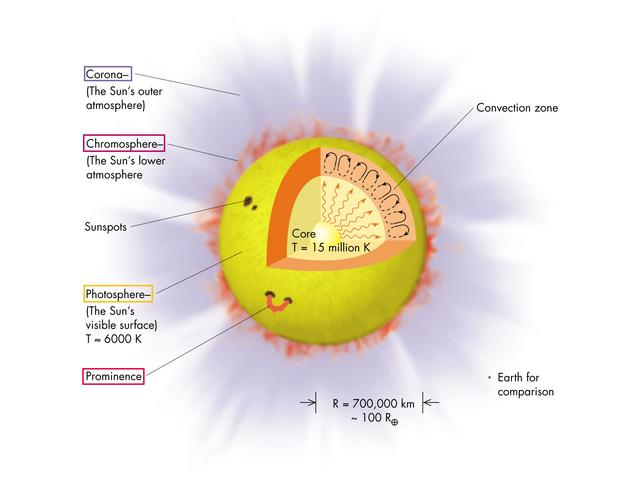
\includegraphics[trim = 0cm 0.5cm 0cm 0cm, width=1.0\textwidth]{images/solar_atmosphere}
\caption{The internal structure of the Sun, including the core, radiative zone, and convective zone.  Also shown is the structure of the its atmosphere, including the photosphere, chromosphere, and corona. The layers of the solar atmosphere are usually demarcated by temperature changes as height above the solar surface increases. The temperature ranges from $\sim$6000\,K in the photosphere to above 1\,MK in the corona.}
\label{fig:solar_atmosphere} 
\end{center}
\end{figure}



\subsection{Solar Dynamo and Magnetic Field}\label{sec:11}

\begin{itemize}
\item Cellular pattern in photosphere is very different to the convective structure in deeper layers.
\end{itemize}


\begin{figure}[!h]
\begin{center}
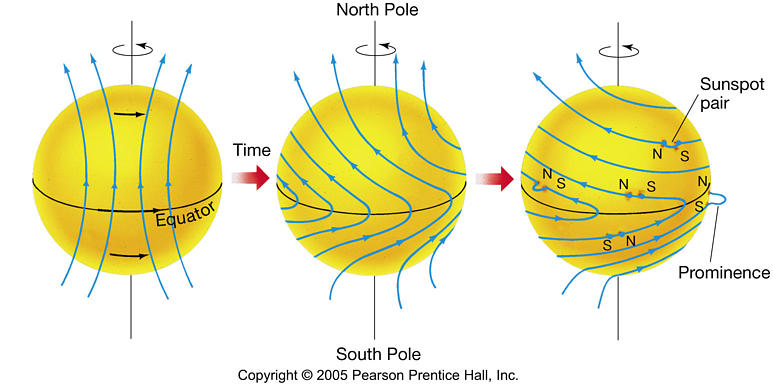
\includegraphics[]{images/Babcock}
\caption{Differential rotation and flux freezing result in the poloidal dipolar magnetic field, generated by dynamo action, to be dragged around in a toroidal direction, an action known as the omega effect. Buoyancy of the field lines results in them rising and twisting, known as the alpha effect, eventually surfacing to become bipolar fields that extend far into the corona.}
\label{fig:Babcock} 
\end{center}
\end{figure}

It is widely believed that the Sun's magnetic field is created by a dynamo action in a region between the radiative zone and the convection zone, known as the tachocline. Solar dynamo theory attempts to explain the observed 11 year magnetic activity cycle, where the the Sun's magnetic field starts as a poloidal dipolar structure and evolves to having a strong toroidal component, after which it returns to a poloidal field again. During these 11 years the Sun starts at minimum activity, reaches a maximum and returns to minimum again.

\citet{babcock1961} first explained this process by a mechanism involving differential rotation of the solar surface and interior. The equatorial rotation rate is faster than the rotation rate at higher latitudes. Because the magnetic field is frozen into the plasma, any flows in the solar interior will tend to drag the magnetic field along. By this effect, differential rotation tends to drag the field and wrap it around the Sun in a toroidal direction, this is known as the omega effect, see Figure~\ref{fig:Babcock}.

As the toroidal field builds up in the solar interior, sections of field lines build up in magnetic pressure resulting in a buoyancy of the field. The field slowly rises through the convection zone and eventually surfaces as a bipolar region that extends into the solar atmosphere. The presence of bipolar fields in the solar atmosphere and their slow build up over time to complex magnetic structures, known as active regions, ultimately leads to a variety of eruptive phenomena.



\subsection{Solar Atmosphere}\label{sec:12}

\subsubsection{Photosphere}\label{sec:121}

\begin{itemize}
\item Appearance, Granules, Sunspots.
\item Black Body Curve. Franhofer lines, H-alpha line, CaII H \& K, H$^{-}$ alines, Sodium D lines. 
\item Temperature, Density, Opacity.
\item Magnetic field strength
\end{itemize}

The most spectacular and energetic phenomena in our solar system have their origins in the solar atmosphere. This ever-changing and dynamic environment is a hotbed of activity giving rise to coronal mass ejections (CMEs), solar flares, and a host of plasma processes resulting in emission across the entire electromagnetic spectrum. To make sense of the phenomena we observe we must first have a basic understanding of solar atmospheric structure and the environment these processes take place in. Figure~\ref{fig:solar_atmosphere} is an illustration of the different layers of the solar interior, the solar surface and atmosphere. The visible surface of the Sun is known as the photosphere. It is demarcated where optical depth becomes unity for a wavelength of 5000\,\AA\ or $\tau_{5000}=1$. At such visible wavelengths, the electromagnetic spectrum is well represented by a blackbody of temperature T$\sim$6000\,K. .

\begin{itemize}
\item Eddington Barbier, $\tau=\mu$, limb darkening.
\item Effective temperature, $\tau=2/3$, $T=5800$\,K
\end{itemize}

During periods of increased activity there may also be the presence of sunspots in the photosphere. These are dark features on the solar surface, see Figure~\ref{fig:solar_atmosphere}, and are an indicator of concentrations of magnetic fields that are stronger than elsewhere in the quiet sun, as described above. 

Photospheric abundances have been measured using emission line diagnostics were it is found that helium is the most abundant at 10.89\footnote{Abundances quoted relative to hydrogen on a logarithmic scale, $12.0+log_{10}(A/A_H)$}, with the next most abundant elements being Carbon (8.58), Nitrogen (8.02), and Oxygen (8.8). All other elements have abundances that are 4 orders of magnitude or more less than hydrogen i.e., logarithmic abundances $\lesssim7$ \citep{phillips2008}.

\subsubsection{Chromosphere}\label{sec:122}

\begin{itemize}
\item Appearance, Supergranular Network, Bright Points, Spicules, Filaments, Plage etc.
\item Emission lines, H-alpha, CaII H \& K. 
\item Temperature, Density, Opacity.
\item Magnetic field strength.
\end{itemize}

At $\sim$500\,km above the $\tau_{5000}=1$ surface the temperature drops to a minimum of $\sim$4400\,K. Beyond this minimum the temperature begins to rise again, demarcating the beginning of the chromosphere. This layer of the atmosphere is generally accepted to extend to a height at which temperatures reach 20,000\,K, however temperatures as high as $\sim1\times10^5$\,K are sometimes attributed to chromospheric heights, hence it is observable at ultraviolet (UV) wavelengths as well as visible. 

\subsubsection{Corona}\label{sec:123}

\begin{itemize}
\item Appearance UV: Active regions, Coronal Loops, Holes.
\item Emission lines, Mg, Ca, Fe, C, O etc.
\item Appearance White-Light: Streamers, K, F, E corona
\item Appearance Radio: thermal bremsstrahlung, free-free emissivity/opacity.
\item Temperature, Density, Opacity, 'coronal heating problem'.
\end{itemize}


At a height of approximately 2,000\,km the temperature begins to rise sharply while the number density of neutral hydrogen and electrons fall by several orders of magnitude. This rapid increase in temperature in such a short spatial extent ($<$100\,km) is known as the transition region. It has a temperature on the order of $10^5$\,K and separates the relatively low temperature chromosphere and the high temperatures of $>1$\,MK in the corona. The reason for this rapid increase in temperature is still a hotly debated subject and a coronal heating mechanism remains largely unknown, this is known as the  \textquoteleft coronal heating problem'.


Element abundances in the corona show there is a similar composition to the photospheric abundances, with He, C, N, and O having the same ratios relative to H in the corona as that in the photosphere. The only difference is an enhancement in the abundance of low First Ionization Potential ($<10$\,eV) elements in the corona relative to the photosphere. For example, elements such as Na, Mg, Al, Si, Ca, Ni, and Fe can be up to three times more abundant in the corona \citep{feldman2003}. The reason for the enhancement of low FIP elements in the corona is still unknown, however several models have suggested ion-neutral separation in the chromosphere by diffusion across magnetic fields, followed by transport of these ions into the corona may be viable mechanism \citep{geiss1985}. 


\subsection{Solar Wind}\label{sec:13}

\begin{itemize}
\item Parker's solution
\item Parker Spiral
\item Fast solar wind, Alfv\'{e}n wave driver
\item Mass loss rates (later compare CME mass loss)
\end{itemize}



\section{Coronal Mass Ejections and Coronal Shocks}\label{sec:2}

\subsection{CMEs}\label{sec:20}

\begin{itemize}
\item Appearance, white-light Illing, Hundhausen, Vourlidas
\item Kinematics, velocity, acceleration
\item Dynamics, masses, energies, forces
\item Observations at other wavelengths, EUV, radio, SXR.
\end{itemize}

\subsection{CMEs and Shocks}\label{sec:21}

\begin{itemize}
\item Radio bursts, Type II, Type III
\item Radio imaging of shocks
\item Relationship to EUV waves, Moreton waves
\end{itemize}

\subsection{Open Questions}\label{sec:22}






	
%!TEX root = ../thesis.tex
%Adding the above line, with the name of your base .tex file (in this case "thesis.tex") will allow you to compile the whole thesis even when working inside one of the chapter tex files
\singlespacing
\chapter{Coronal Mass Ejection and Plasma Shock Theory} 
\label{chap:2}
\doublespacing
This chapter introduces the theory used to study coronal mass ejections and coronal shocks. Since the corona is a plasma, the theoretical framework under which all coronal phenomena are treated is in plasma physics and a fluid description of plasmas known as magnetohydrodynamics (MHD). Coronal mass ejections are a large scale phenomena and can therefore be treated using MHD. While plasma shocks on the large scale may also be treated in an MHD continuum framework, it is necessary to consider individual particle motions when describing particle acceleration and radio emission in shocks, requiring a departure from MHD and the use of distribution functions, the Boltzmann equation, and individual particle kinematics. Therefore, both the MHD equations and the Boltzmann equation are presented in this chapter, followed by an application of this theory to CMEs and plasma shocks.

\singlespacing
\section{Plasma Physics and  \\ Magnetohydrodynamics}\label{sec:1}
\doublespacing
\subsection{Maxwell's Equations}\label{sec:10}

Since plasmas are an electrically conducting fluid which may interact with electromagnetic fields, Maxwell's equations are an essential starting point for all plasma theory. Maxwell's equations form a closed set of four unknowns and four equations describing relationships between the electric field $\mathbf{E}$, the magnetic field $\mathbf{B}$, the current density $\mathbf{j}$, and the charge density $\rho_q$
\begin{eqnarray}
\nabla \cdot \mathbf{E} &=& \frac{\rho_q}{\epsilon_0} \\
\nabla \cdot \mathbf{B} &=& 0 \\
\curl{\mathbf{E}} &=& - \frac{d\mathbf{B}}{dt} \\
\curl{\mathbf{B}} &=& \mu_0 \mathbf{j} + \frac{1}{c^2}\frac{d\mathbf{E}}{dt} 
\end{eqnarray}
$\mu_0$ and $\epsilon_0$ are the magnetic permeability and electric permittivity of free space, respectively, and all bold face quantities represent vector variables. At velocities typically found in a plasma equation (2.4), Amp\'{e}re's law, reduces to
\begin{equation}
\curl{\mathbf{B}} = \mu_0 \mathbf{j}
\end{equation}
where the displacement current is no longer included. Maxwell's equations describe electromagnetic behaviour and they constitute an important part of the fluid description of plasmas. Before we define this fluid description a brief discussion of plasma kinetic theory, from which the fluid theory is derived, is provided here.

\subsection{Plasma Kinetic Theory}\label{sec:11}

The general approach to the majority of plasma phenomenon is in a collective description using particle distribution functions and the use of differential equations to describe the evolution of these distribution functions. This is known as plasma kinetic theory, and the distribution functions can be of the form of the Maxwell-Boltzmann velocity distribution, while the differential equation used to describe its evolution is the Boltzmann equation. Many non-equilibrium or unstable states of a plasma, such as those that produce radio bursts described in sections~\ref{sec:wave_particle}--\ref{sec:three_wave} require a kinetic theory description of plasma. A brief overview of kinetic theory is therefore given here before describing specifically its application to plasma emission and radio bursts.

As with a neutral gas, the particle distribution function $f(\mathbf{r}, \mathbf{v}, t)d\mathbf{v}d\mathbf{r}$ described the number of particles having positions between $\mathbf{r}$ and $\mathbf{r}+d\mathbf{r}$ and velocities between $\mathbf{v}$ and $\mathbf{v}+d\mathbf{v}$, at time $t$. This distribution function can be used derive a number of useful physical properties of the plasma, such as the particle number density at position $\mathbf{r}$ and time $t$ 
\begin{equation}
n(\mathbf{r},t) = \int f(\mathbf{r}, \mathbf{v},t) d \mathbf{v}
\label{eqn:num_density}
\end{equation}
as well as the bulk velocity particle velocity, given by
\begin{equation}
 \mathbf{v}(\mathbf{r},t) = \frac{1}{n(\mathbf{r},t)}\int  \mathbf{v} f(\mathbf{r}, \mathbf{v},t) d \mathbf{v}
\label{eqn:bulk_flow}
\end{equation}
The evolution of this distribution function in time and space is described by the Boltzmann equation, given by
\begin{equation}
\frac{\partial f(\mathbf{r}, \mathbf{v},t)}{\partial t}  +     ( \mathbf{v}\cdot\nabla_r)f(\mathbf{r}, \mathbf{v},t)    + (\mathbf{a}\cdot\nabla_v)f(\mathbf{r}, \mathbf{v},t) = \bigg(\frac{\partial f(\mathbf{r}, \mathbf{v},t)}{\partial t}\bigg)_{coll}
\label{eqn:boltzmann}
\end{equation}
This equation describes the changes in occupation number of particles at positions ($\mathbf{r}, \mathbf{v}$, t) in phase space due to a configuration space flux $\mathbf{v}\cdot\nabla_rf$, a velocity space flux $ \mathbf{a}\cdot\nabla_vf$, as well as collisions experienced by the particles (last term in the right). Equation~\ref{eqn:boltzmann} is the fundamental basis of all plasma and neutral gas kinetic theory and provides a very powerful tool for describing the time and space evolution of equilibrium and, more importantly, non-equilibrium distributions of particles. It is the most general description of the behavior of an ensemble of particles, and all other macroscopic fluid dynamical equations may be derived from it.

Assuming  the plasma to be collisionless and stating the accelerations in the plasma in terms of the electric field $\mathbf{E}$ and magnetic field $\mathbf{B}$, Equation~\ref{eqn:boltzmann} may be reduced to the Vlasov equation for a plasma interacting with electromagnetic fields.
\begin{equation}
\frac{\partial f}{\partial t}  +(\mathbf{v}\cdot\nabla_r)f + (\frac{q}{m}[\mathbf{E} + \mathbf{v}\times \mathbf{B}]\cdot\nabla_v)f = 0
\end{equation}
where $q$ is Coulomb charge, $m$ is particle mass, and $f(\mathbf{r}, \mathbf{v},t)$ is reduced to $f$ for simplicity of notation. This form of the Vlasov equation is used in the formulation of wave-particle interactions, and wave growth in plasmas, that ultimately lead to plasma emission in solar radio bursts, this will be described in further detail sections~\ref{sec:wave_particle}--\ref{sec:three_wave}.

In equations \ref{eqn:num_density} and \ref{eqn:bulk_flow}, the number density and bulk velocity of the plasma were obtained by taking appropriate weighted integrals of the distribution function. This is done to obtain information on the macroscopic properties of the plasma when the specific details of the particle distribution are not needed. A behaviour of the plasma on a macroscopic or fluid scale may be obtained by taking the appropriate integrals of the the Boltzmann equation in a procedure known as `taking the moments of the Boltzmann equation'. The moments of a function are given by 
\begin{equation}
\mu_n = \int x^n f(x) dx
\end{equation}
where the $n$ describe the moments e.g., $n=0$ is the {\it zeroth moment},  $n=1$ is the {\it first moment} etc. Taking the moments of the Boltzmann equation lead to a set of fluid conservation equations that describe the dynamics of a plasma on a continuum scale (no individual particle motion available). The moments are as follows
\begin{eqnarray*}
\int [\mathrm{Boltzmann~ eq.}]\times v^0 dv &\rightarrow& \mathrm{conservation~of~mass} \\
\int [\mathrm{Boltzmann~eq.}]\times v^1 dv &\rightarrow& \mathrm{conservation~of~momentum} \\
\int [\mathrm{Boltzmann~eq.}]\times \frac{v^2}{m} dv &\rightarrow& \mathrm{conservation~of~energy}
\end{eqnarray*}
In their most fundamental form, these conservation equations are used in what is known as a multi-fluid description of the plasma, where the dynamics and conservations of the various properties are treated seperately for each particle species e.g., electrons and protons will have different conservation equations and described separately as an \textquoteleft electron fluid' and \textquoteleft proton fluid'. However, combining these separate fluids into one \textquoteleft single fluid' framework constitutes a description of plasmas known as magnetohydrodynamics\footnote{The moments of the distribution function and the reduction of multi-fluid to single fluid conservation equations involve lengthy derivations that are not provided here but can be found in many texts \citep{goossens2003, inan2011}.}.

\subsection{Magnetohydrodynamics}\label{sec:12}
The conservation principles  derived from moments of the Boltzmann equation are firstly the mass conservation equation
\begin{equation}
\frac{D\rho}{Dt} = -\rho\nabla\cdot \mathbf{v}
\end{equation}
where $\rho$ is mass density, $\mathbf{v}$ is bulk flow velocity, $t$ is time, and $D$ represents a Lagrangian derivative ($D/Dt = \partial /\partial t + v\cdot \nabla$). This expression simply states that the rate of change of particles into or out of a volume is controlled by the fluid flow into and out of the volume. It has units of kg\,m$^{-3}$\,s$^{-1}$.

Secondly, the momentum conservation equation is
\begin{equation}
\rho\frac{D\mathbf{v}}{Dt}=-\nabla p + \mathbf{j}\times \mathbf{B} + \mathbf{f} +\nabla \cdot \mathbf{S}
\label{eqn:mhd_momentum}
\end{equation}
where $p$ is thermal pressure, $\mathbf{j}$ is the current density, $\mathbf{B}$ is the magnetic field, $\mathbf{f}$ are all body forces e.g., gravity, and $\mathbf{S}$ is a stress tensor. This equation shows that the change in momentum of a fluid may be due to a pressure gradient, the \textquoteleft j cross B' or Lorentz force, gravity, and any stresses in the plasma e.g., kinematic viscosity $\nu$. Note that with $\nabla \cdot \mathbf{S}=\rho\nu\nabla^2\mathbf{v} $, and setting gravity and the Lorentz term to zero gives the Navier-Stokes equation of motion of a viscous fluid. Note that all terms in this equation have the form of a body force (force per unit volume), and integration over volume would render this equation an explicit version of Newton's second law ($m\mathbf{a}=\mathbf{F}$).

The third conservation equation is the energy conservation equation
\begin{equation}
\rho\frac{De}{Dt} + p\nabla\cdot \mathbf{v}=\nabla\cdot(\kappa\cdot\nabla T) +  \eta_e\mathbf{j}^2 + Q_{\nu} - Q_r
\end{equation}
where 
\begin{equation}
e = \frac{p}{(\gamma-1)\rho}
\end{equation}
is the internal energy per unit mass, $\gamma$ is the ratio of specific heats, $\kappa$ is the thermal conductivity, $T$ is the temperature, $\eta_e$ is electrical resistivity, $Q_{\nu}$ is heating by viscous dissipation, and $Q_r$ is a radiative term. This equation demonstrates that any changes in the fluid internal energy are due to divergence in the flow field, conduction, ohmic and vicious dissipation, and radiative losses.

The fluid momentum equations can be used to formulate Ohm's law for a plasma which describes the behaviour of current in terms of electric and magnetic fields and the fluid flow velocity
\begin{equation}
\mathbf{j} = \sigma(\mathbf{E} + \mathbf{v}\times \mathbf{B})
\end{equation}
This is a reduced version of the generalised Ohm's law and does not contains terms for the Hall effect, ambipolar diffusion, and electron intertia. The set of equations (2.11 - 2.15), combined with an equation of state 
\begin{equation}
p = nk_BT
\end{equation}
results in a fully closed set of variables and equations, which can be solved for any fluid or electromagnetic property. In order to further simplify these set of equations the electric field $\mathbf{E}$ and current $\mathbf{j}$ are often eliminated by using Faraday's law in combinations with Amp\'{e}re's and Ohm's law to produce the induction equation
\begin{equation}
\frac{\partial \mathbf{B}}{\partial t} = \nabla \times(\mathbf{v}\times \mathbf{B}) + \eta\nabla^2 \mathbf{B}
\end{equation}
which describes the evolution of the magnetic field in terms of the plasma flow and the magnetic diffusivity $\eta = \eta_e/\mu_0$.  The mass, momentum, internal energy equation, the induction equation, and the solinoidal constraint then define  a fully closed system of resistive MHD equations in terms of the variables ($\mathbf{B}, \mathbf{v}, p, \rho$)
\begin{eqnarray}
\frac{D\rho}{Dt} = -\rho\nabla\cdot \mathbf{v} \\
\rho\frac{D\mathbf{v}}{Dt}=-\nabla p + \frac{1}{\mu_0}(\nabla \times \mathbf{B})\times \mathbf{B} + \mathbf{f} \\
\frac{D\rho}{Dt} = -\gamma p\nabla\cdot \mathbf{v} +(\gamma -1)\frac{\eta}{\mu_0^2} (\nabla \times \mathbf{B})^2 \\
\frac{\partial \mathbf{B}}{\partial t} = \nabla \times(\mathbf{v}\times \mathbf{B}) + \eta\nabla^2 \mathbf{B} \\
\nabla\cdot \mathbf{B} = 0
\end{eqnarray}
It is also assumed here that the fluid is inviscid and not subject to any conductive or radiative energy losses or gains. Under this reduced set of equations, the ideal MHD equations are simply produced by setting $\eta = 0$ e.g., zero resistivity, which would eliminate the second terms on the right in equations 2.20 and 2.10. Under such an assumption the ideal induction equation
\begin{equation}
\frac{\partial \mathbf{B}}{\partial t} = \nabla \times(\mathbf{v}\times \mathbf{B})
\end{equation}
may be used to show the \textquoteleft frozen flux' condition. This shows that when $\eta = 0$ the field is advected with the plasma or the field is \textquoteleft frozen-in' into the plasma and follows the flow velocity i.e., there is no `slipping' of the magnetic field with respect to the fluid flow.  On the other hand, a finite $\eta$ leads to a variety of important diffusive effects for the magnetic field. The most important of these diffusive processes is magnetic reconnection, which plays an extremely important role in solar flares and CMEs.



%-----------------------------------------------------------%
%		   Magnetic Reconnection	                 % 
%-----------------------------------------------------------%
\subsection{Magnetic Reconnection}\label{sec:13}

If the dissipation of concentrations of magnetic flux in the solar corona are due to diffusion processes only, a timescale for this diffusion process may be estimated from the magnetic induction equation. Assuming the diffusion term dominates over advection term
\begin{equation}
\frac{\partial B}{\partial t} = \eta\nabla^2\mathbf{B}
\label{egn:diff}
\end{equation}
As an order of magnitiude estimate for the derivatives we replace $\partial/\partial t \rightarrow 1/\tau_D$ and $\nabla^2 \rightarrow 1/L^2$. Equation~\ref{egn:diff} then gives
\begin{equation}
\tau_D = \frac{L^2}{\eta}
\label{eqn:diff_time}
\end{equation}
The typical length scales for a coronal active region are $10^7$\,m, and assuming a Spitzer magnetic diffusivity $\eta = 10^9T^{-3/2} = 1$\,m$^2$\,s$^{-1}$ \citep{spitzer1962}, equation~\ref{eqn:diff_time} gives a diffusive timescale of 3.1 million years.
Given that active regions evolve quasi-statically over weeks and evolve dynamically over timescales of seconds and minutes during a flares and CMEs, there must be an evolution process other than a large scale diffusion in the solar atmosphere. Equation~\ref{eqn:diff_time} indicates that there may be two different ways in which the evolution of magnetic fields may occur over a much shorter times scale: either the typical length scale $L$ is much shorter, or magnetic diffusivity $\eta$ is much larger.

Magnetic reconnection is the dynamical process that describes the short timescale evolution of magnetic fields in the corona (and other astrophysical and laboratory systems). It involves a change in magnetic topology that converts magnetic energy in kinetic and thermal energy of the bulk plasma and accelerates particles to high speeds. Magnetic reconnection typically occurs in a boundary between two oppositely directed magnetic field regions. At the very center of the boundary layer the magnetic field must go to zero to account for a continuous change from positive to negative magnetic field. The total pressure balance in the boundary layer and on either side is \citep{asch2004}
\begin{equation}
B_1 + p_1 = p_{dr} = B_2 + p_2
\end{equation}
where $p_{1,2}$ and $B_{1,2}$ represent thermal and magnetic pressure on either side of the diffusion region, respectively, and $p_{dr}$ is the pressure inside the diffusion region (no magnetic pressure).


\begin{figure}[!t]
\begin{center}
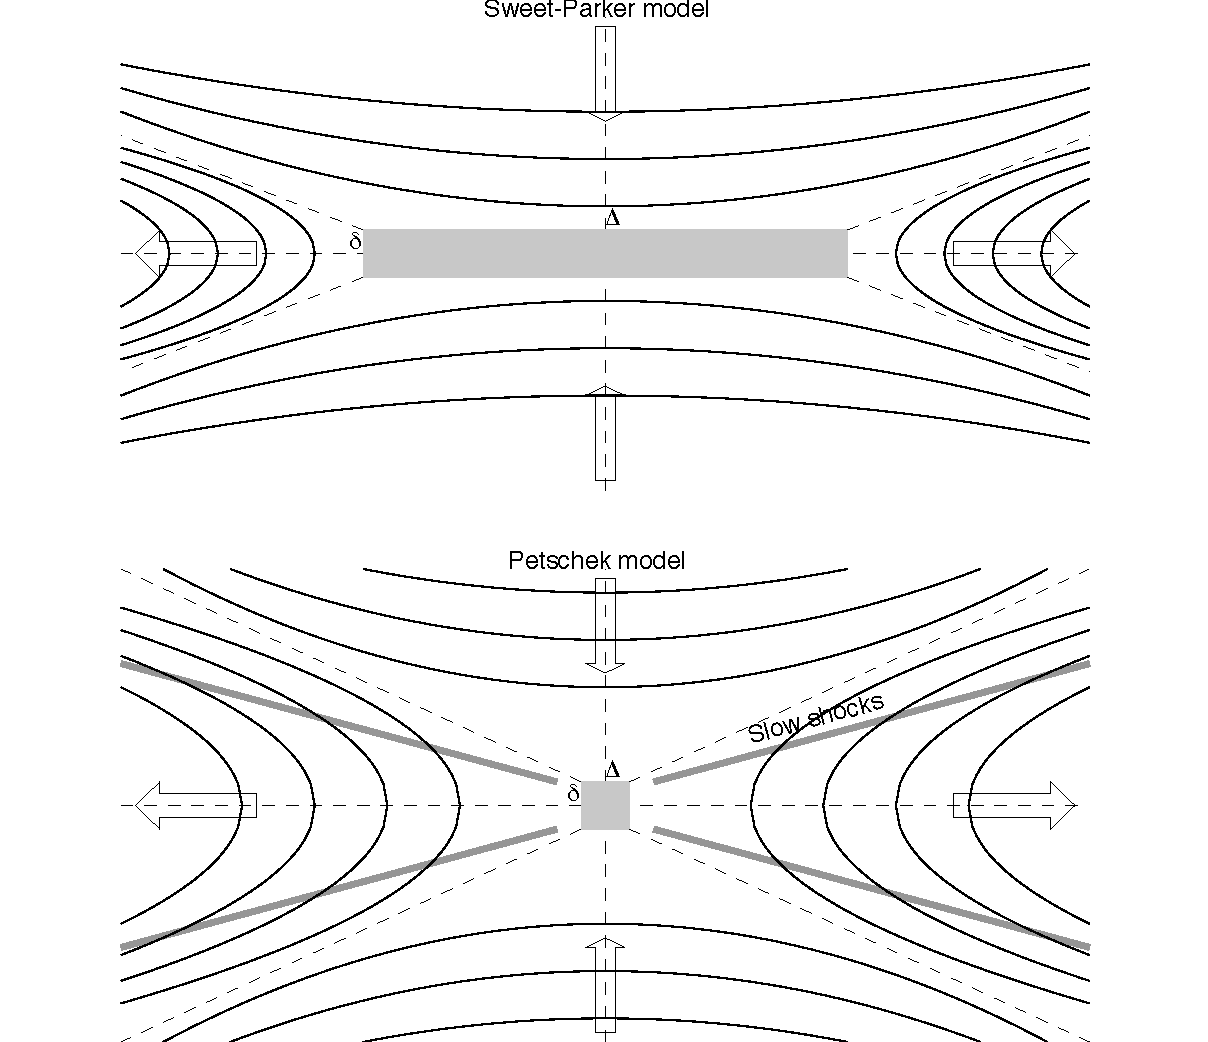
\includegraphics[scale=0.7]{reconnection.pdf}
\caption[Sweet-Parker and Petscheck reconnection models]{The reconnection models of Swee-Parker (top) and Petscheck (bottom). The Sweet-Parker mechanism employs a long and thin ($\Delta>>\delta$) current sheet as the diffusion region. It produces reconnection rates that are much too slow to describe flare and CME energy dissipations rates. Petscheck proposed a similar model but with a diffusion region that is much smaller, with $\Delta\approx\delta$, resulting in reconnection rates that are consistent with flare and CME timescales. The dissipation of energy in this model is partly controlled by the presence of two slow-mode shocks which separate the sub-Alfv\'{e}nic inflow region and the super-Alfv\'{e}nic outflow region \citep{asch2004}.}
\label{fig:recconection}
\end{center}
\end{figure}
The existence of inflows into the diffusion region at right angles to the magnetic field creates an electric field in this layer that is perpendicular to the inflow plane. This creates a current in the diffusion region, hence this ayer is often called a `current sheet'. The diffusion of magnetic fields occurs within this current sheet. Sweet and Parker were the first devise a mechanism by which magnetic reconnection occurs in such a current sheet \cite{sweet1958, parker1963}. 
%Although no complete analytical theory exists for the process, the MHD conservation equations may be applied to derive the reconnection rate. The application of resistive MHD only applies within the thin current sheet, while ideal MHD applies everywhere else.

The Sweet-Parker were the first to devise a model whereby the diffusive time scale of the field (equation~\ref{eqn:diff_time}) could be made much faster by considering a diffusion region much smaller than the size scales of active regions. The model consists of a current sheet (diffusion region) that is much longer than it is wide i.e., in the top panel of Figure~\ref{fig:recconection} $\Delta>>\delta$, where $\Delta$ is current sheet half-length and $\delta$ is current sheet half-thickness. Conservation of mass implies that the rate at which mass enters the sheet must equal the rate that mass exits the sheet
\begin{equation}
\rho \Delta v_{in} = \rho \delta v_{out}
\label{eqn:in_out}
\end{equation}
where $v_{in}$ and $v_{out}$ are the inflow and outflow speeds respectively. Using equations~\ref{eqn:diff_time} and \ref{eqn:in_out} the inflow speed may be written as
\begin{equation}
v_{in}^2 = \frac{\eta v_{out}}{L}
\end{equation}
The reconnection rate depends on in the ratio of the inflow speed $v_{in}$ to the outflow speed $v_{out}$ in the form of the Mach number
\begin{equation}
M = \frac{v_{in}}{v_{out}} = \frac{1}{\sqrt{S}}
\end{equation}
where $S=v_AL/\eta$ is the Lundquist number (equivalent to the magnetic Reynold's number at the Alfv\'{e}n speed). The rate of reconnection depends on the length scale and magnetic diffusivity in the current sheet. Despite the fact that the Sweet-Parker mechanism provides a rate of magnetic energy dissipation that is faster than the global process, it is much too slow to explain the process of magnetic energy release in solar flares. For example for typical Lundquist numbers of $10^{12}$, the Sweet-Parker model produces a reconnection rate of $10^{-6}$ of the Alfv\'{e}n speed.

To over come the problem, Petscheck proposed a model with a much smaller diffusion region where $L\approx\delta$ \citep{petschek1964} . With this smaller diffusion region, the boundary between inflow and outflow regions are separated by slow mode magnetoacoustic shocks. Alongside the diffusion region, these shocks also help to dissipate some of the inflowing kinetic energy into thermal energy. Again, no analytical solution to the model exists but Petscheck found that when the diffusion regions is allowed to be small, the reconnection rate is given as
\begin{equation}
M \approx \frac{\pi}{8\,\mathrm{ln}(S)}
\end{equation}
This gives a much faster reconnection rate of 0.01 of the Alfv\'{e}n speed (hence it is known as fast reconnection), which is comparable to solar flares. When Petscheck presented the model it was thought to be a complete description of 2D magnetic reconnection, however other solutions would soon be discovered, with the Petscheck model being just one of a family of possible 2D reconnection mechanisms. These mechanisms describe steady, uniform, 2D reconnection, the rate of which may be summarised as \citep{priest1986}
\begin{equation}
\bigg(\frac{M_e}{M_e}\bigg)^2 \approx \frac{4M_e(1-b)}{\pi}\bigg[ 0.834 -\mathrm{ln \, tan}\bigg( \frac {4S\sqrt{M_eM_i}} {\pi}  \bigg)^{-1}\bigg]
\end{equation}
This contains the Sweet-Parker, the Petscheck ($b=0$) and Sonnerup \citep{sonnerup1970}($b=1$) reconnection rates.

%While these solutions show that 2D reconnection may be explained well by MHD, describing 3D reconnection remains big theoretical and computational challenge, and remains at the forefront of reconnection theory research. Both 
2D reconnection, an the more complicated 3D models, play a role in many theoretical models describing the eruption of coronal mass ejections and flares. Although some CME models have no need for reconnection to occur, there is a growing consensus that it is an integral part of the solar eruptive process.

%-----------------------------------------------------------%
%		       CME Theory			        % 
%-----------------------------------------------------------%

\section{Coronal Mass Ejections}\label{sec:2}

Magnetohydrodynamic models of eruptive coronal mass ejections use either ideal or resistive MHD (without and with reconnection, respectively) to bring about a loss of equilibrium of some complex magnetic structure in the corona. The magnetic structure usually takes the form of a flux rope, a helical or twisted magnetic structure embedded in the coronal magnetic field. The main goal of every model is to induce a loss of equilibrium of the structure, but the mechanism by which this is done varies greatly amongst the models. {\it Storage models} assume a slow build up of magnetic stress in a non-potential field that may store free energy over long time scales before some loss of equilibrium occurs and the stored magnetic energy is rapidly converted to mechanical energy and the expulsion of a magnetic structure \citep{wolfson1998, forbes1995, antiochos1999}. {\it Dynamo models} involve a rapid generation of magnetic flux by either stressing of the field or flux-injection into the system. As the name suggests, these models usually consider the interplay between current and magnetic field in the system that may bring about a Lorentz force which provides an expulsion of the flux rope from the low corona \citep{chen1989, krall2001, schrijver2008, fan2005}. Finally there are the {\it thermal blast models}, which produce an expulsion of the CME into interplanetary space by an enhanced pressure gradient due to the rapid heating of a flare i.e., an explosive ejection of plasma from the corona.  This model is somewhat out-dated now since CMEs are no longer thought to be the result of flares, with some CMEs preceding flare onset and some occurring without any flare \citep{gosling1993}.

The main goal of every model is to induce a loss of equilibrium of the structure, but the mechanism by which this is done varies greatly amongst the models e.g., there is still some debate on whether the flux rope is formed as a result of eruption or it is a pre-existing structure. The need for reconnection is also a source of contention, with some models inducing eruption using only ideal MHD and other models employing resistive MHD \citep{chen2011}. The most prominent of these models are discussed here.

\subsection{Catastrophe Model}\label{sec:20}
\begin{figure}[!t]
\begin{center}
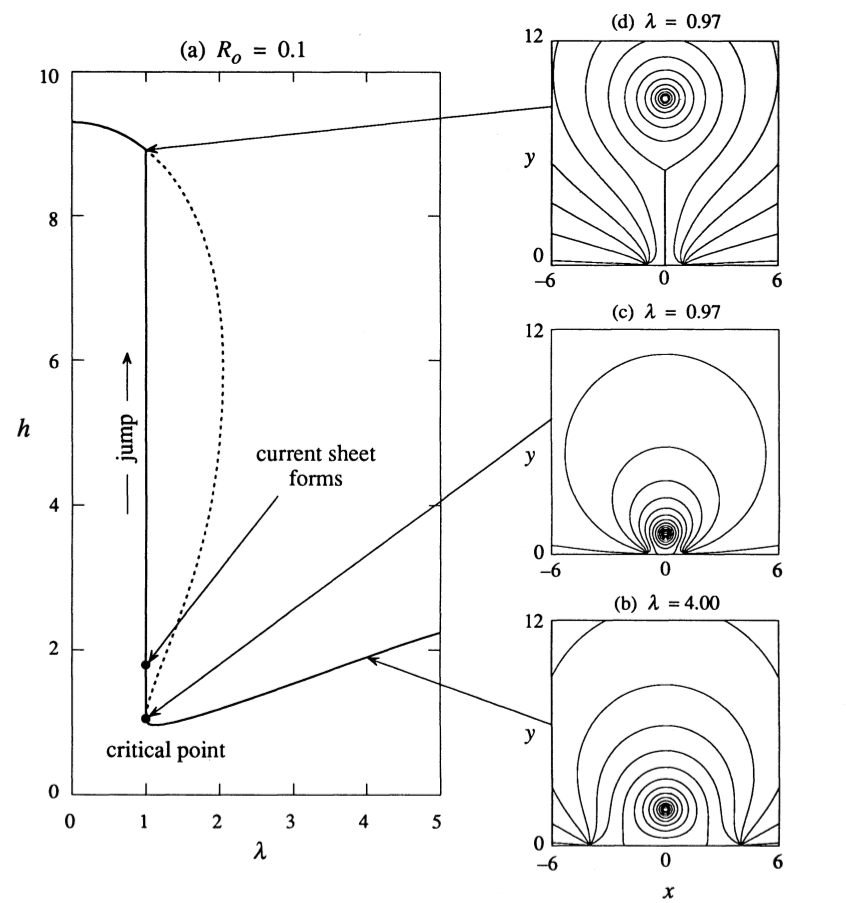
\includegraphics[scale=0.4, trim=1cm 1cm 0cm 1.5cm]{images/catastrophe}
\caption[The catastrophe CME model]{The catastrophe model of \citep{forbes1995}. The model consists of a 2D pre-existing flux rope with foot points rooted in the photosphere. The fluxrope is driven toward instability by motions of the photospheric footpoints, in this case the distance between the footpoints $\lambda$ decreases slowly (timescales much longer than the Alfv\'{e}n crossing time $\tau=L/v_A$). As the foot points converge the fluxrope initially contracts indicated by a decreasing height in panel (a). Eventually this convergence brings the system to critical point where magnetic pressure outwards dominates inward magnetic tension. The system rises, reaches a new equilibrium position, and forms a current sheet. The evolution of the system after it reaches this new equilibrium largely depends on whether or not magnetic reconnection occurs in the sheet. the rate of reconnection may also bring about different evolutions in kinematics \citep{priest2000}.}
\label{fig:catastrophe}
\end{center}
\end{figure}

The catastrophe model assumes a flux-rope is formed in the corona prior to eruption and considers the balance between magnetic tension holding the flux rope in position, and magnetic pressure (from compression of field lines under the rope) that supply an outward directed force \citep{forbes1991, lin2000, priest2000}. A loss of equilibrium is brought about by photospheric motions, either convergence or shearing of the foot points, which are well-known precursors to eruptive activity in the corona \citep{rust1972}. the reduction of the distances between the foot points, $2\lambda$, decreases and this initially 
causes an increase in the magnetic tension which makes the rope contract and reduce its height Fig.~\ref{fig:catastrophe}. However, continued contraction results in a magnetic compression that  dominates tension, resulting in a flux rope rise. As the rope rises it forms a current sheet behind it, and its evolution after this point depends on whether or not reconnection occurs in the current sheet. If no reconnection is present then the flux rope simply rises and finds a new equilibrium position at a greater height, in this case the net release of magnetic energy is less than 1\% of the energy stored in the pre-field configuration \citep{forbes1991}. If reconnection occurs, then the eruption proceeds uninhibited and up to 95\% of the stored magnetic energy is released \citep{forbes1995}.

\citet{forbes1995} provided expressions for the development of current in the flux rope with respect to height which was used to estimate the free magnetic energy in the system. By assuming a rapid reconnection rate, and that all of this free energy was converted to the rope's kinetic energy they were able to derive velocity-time kinematics, and under the constraint of the flux rope radius $a\rightarrow 0$ an analytical expression for the rope velocity may be derived as \citep{priest2000}
\begin{equation}
v\approx \sqrt{  \frac{8}{\pi}  }v_{A0}\bigg[\mathrm{ln}\bigg( \frac{h}{\lambda_0}\bigg) + \frac{\pi}{2}  - 2\mathrm{tan}^{-1} \bigg( \frac{h}{\lambda_0}\bigg)\bigg] + v_0
\end{equation}
where $h$ is the fluxrope height, $2\lambda_0$ is the foot point separation at $\lambda=h$, $v_0$ is an initial perturbation velocity (1\% of the Alfv\'{e}n speed), and $v_{A0}$ is the Alfv\'{e}n speed where $\lambda=h$. Magnetic power output in the early phase of eruption is given by
\begin{equation}
\frac{dW}{dt} \approx -\frac{2A_0^2}{\pi\mu}\bigg( \frac{h}{\lambda_0} -1\bigg)^2\frac{v}{\lambda_0}
\end{equation}
where $h\sim t + t^{5/2}$ and $v\sim t^{3/2}$ i.e., the initial power output grows with time. In the later phases of propagation the power output decays with time as
\begin{equation}
\frac{dW}{dt} \approx \frac{4A_0^2}{\pi \mu t}
\end{equation}
so the growth in power output occurs approximately 100 times quicker than the decay in power output.

A later study by \citet{priest2000} analysed how reconnection in the underlying current sheet may influence the eruption of the flux rope. The kinematics of the rope after equilibrium is lost depend on the rate of reconnection in the sheet, parameterised by the Alfv\'{e}n Mach number of the inflow into the reconnection site. If $M_A=0$ then the fluxrope does not escape but oscillates around an equilbrium height like a yo-yo. If $0<M_A<0.005$, escape is possible but the rope may show a number of oscillations in height before escape, this behaviour has never been directly observed so reconnection must occur at a rate $M_A>0.005$ to produce eruption.  For $0.005<M_A<0.041$ to rope escapes but undergoes a period of deceleration between 20 and 100 Alfv\'{e}n crossing times, while for $M_A > 0.041$ no deceleration occurs and the fluxrope escapes and approaches an asymptotic velocity.

The catastrophe model provides a successful way of evolving a flux system to the point of catastrophic loss of equilibrium and consequent eruption. However, a major limitation is that it is a 2D model and does not take into account that the ends of the flux rope will be anchored in the photosphere. This would produce a curvature in the rope that would increase its tension and hence change the dynamics, but it is unlikely that it would prevent eruption \citep{steele1989}




\subsection{Magnetic Breakout Model}\label{sec:21}

The magnetic breakout model was first proposed by \citep{antiochos1999} and involves a quadrupolar (or more complex) magnetic flux system. A core magnetic field is flanked by two side-lobe fields, which collectively lie underneath an over-arching field that stabilizes the whole system. The overarching field and core field are almost anti-parallel, creating a magnetic null point between the two Figure~\ref{fig:breakout_model}. Non potentiality is injected into the core by twisting/shearing of the foot points or by flux emergence. This non-potentiality causes the core field to grow and encounter the overarching field, distorting the null point into a current sheet and eventually allowing reconnection to occur. The reconnection removes field lines from the overarching field and adds it to the side-lobe systems, allowing further growth of the core field. The growth of the core field in turn drives further breakout reconnection resulting in a positive feedback required for explosive expulsion of the core. Finally, as the core is accelerated a current sheet forms in its wake, eventually leading to a separation of the core flux from the solar surface that forms a plasmoid structure typical of a three part CME \citep{lynch2004}; an important aspect of this is that flux rope formation happens as a consequence of eruption i.e., it is not pre-existing. The magnetic breakout model was used to circumvent the Aly-Sturrock limit \citep{aly1991, sturrock1991} i.e., it allowed a flux system to erupt, without having to open the constraining field lines to infinity.
\begin{figure}[!t]
\begin{center}
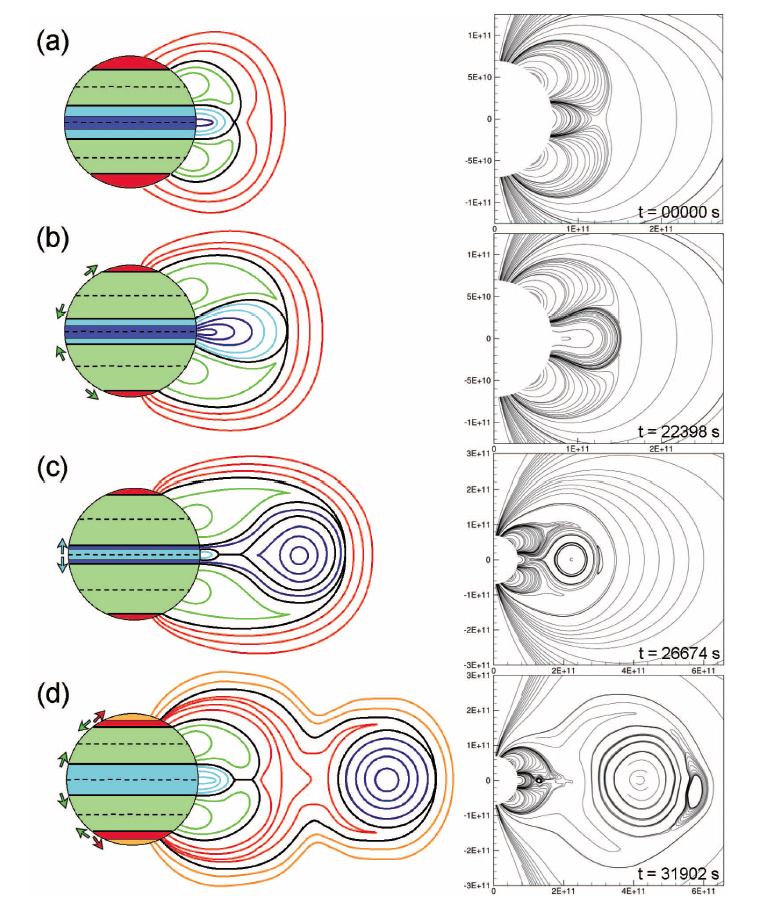
\includegraphics[scale=0.45, trim=0cm 0cm 0cm 1cm]{images/lynch_breakout}
\caption[The breakout CME model]{The breakout model, consisting of a quadrupolar flux system in which the central flux (blue) is flanked by to side lobe flux systems (green), with the entire system kept in stability by the tension of the overlying red field. Shearing and/or twisting on the underlying flux causes it to grow slowly. Eventually a current sheet forms at the magnetic null above the central flux, causing reconnection. This reconnection transfers overlying field to the side-lobes, effectively creating a conduit for the central flux to escape as a CME \citep{lynch2008}.}
\label{fig:breakout_model}
\end{center}
\end{figure}

Kinematically, the CME/central field system should experience a slow rise (1\,km\,s$^{-1}$) for several hours due to shearing/twisting of the foot points. Once breakout reconnection has begun the CME experiences a much larger acceleration (100\,km\,s$^{-1}$). The reconnection in the current sheet in the wake of the CME is the source of energetic particles that ultimately lead to flaring (ribbons and soft x-ray loops). Therefore magnetic breakout predicts that the flaring process and SXR peak should only begin after CME acceleration (after breakout reconnection) has begun \citep{lynch2004}. However, the precedence in breakout reconnection over flaring reconnection may not always be case, with the latter sometimes driving the former \citep{macneice2004}. The above studies have mainly been through 2.5\,D simulations but a 3\,D simulation of the breakout model was given in \citep{lynch2008}. This allowed a full estimate of the conversion of magnetic energy into kinetic energy. It is found that during the flare impulsive phase 17.8\% of the free magnetic energy ($4.6\times10^{31}$\,ergs) is converted into plasma kinetic energy ($8.1\times10^{30}$\,ergs). During the gradual phase the proportion of free magnetic energy converted to kinetic energy drops to 15.4\%

There has been observational tests of the magnetic-breakout model, showing it to be a viable explanation of some flaring and CME events, the most notable of which is the Bastille Day event \citep{aulan2000}. The observational signatures of the model include the presence of a null point in the corona above a complex multipolar flux system (inferred from potential field source surface extrapolations), a radio source imaged to be above the erupting structure (implying a reconnection site), and radio bursts beginning at frequencies indicative of high altitude (again indicating energy release above the erupting structure, prior to eruption) \citep{manoh2003}. However, in some instances magnetic breakout is implied by observations of the above, but the kinematics are inconsistent with model predictions. For example the model predicts a long slow rise of the central flux system as the underlying field is increasingly sheared, after which there is a rapid acceleration once breakout reconnection is initiated. However, in the study of \citet{bong2006} the breakout reconnection occurred at the end of the CME acceleration phase, prompting a two-phase acceleration scenario.


\subsection{Toroidal Instability}\label{sec:22}

The toroidal instability model incorporates a pre-existing flux rope structure that is built from a torus of magnetic flux, some of which is buried beneath the photosphere \citep{chen1989}. The flux system is can be broken down into a combination of toroidal magnetic field, toroidal current , poloidal magnetic field and poloidal current Figure~\ref{fig:chen_model}. This flux rope system is embedded in a surrounding coronal magnetic field $\mathbf{B}_{corona}$. The stability of the system depends on the nature of the $\mathbf{J} \times \mathbf{B}$ force due to the interaction toroidal and poloidal components of both the field and current. The interaction of $\mathbf{J}$ and $\mathbf{B}$ internal to the flux rope is usually termed the Lorentz self-force or the \textquoteleft hoop' force. An instability may be induced via twisting of the fluxrope footpoints to increases the amount of poloidal flux (effectively increasing the helicity of the system). The instability arrises when the outward hoop force decreses more slowly within the ring radius than the opposing Lorentz force due to an external magnetic field. Once the instability is induced, the fluxrope begins a bulk motion as well as a growth in its semi-minor axis. Hence the motion of the system can be analysed by looking at the central axis or the minor axes (leading and trailing edges). The three axes display slightly different kinematics e.g., the leading edge has a faster velocity than the trailing edge (due to fluxrope expansion). This has proved a useful test of the model when comparing the observations of erupting fluxrope structures as seen in white-light coronagraphs. \citet{krall2001} analysed the leading and trailing edges of erupting flux rope, as well as the rope aspect ratio, and compared the observations to model expectations. Good agreement is found between the model kinematics and aspect ratio and the observed events.
\begin{figure}[!t]
\begin{center}
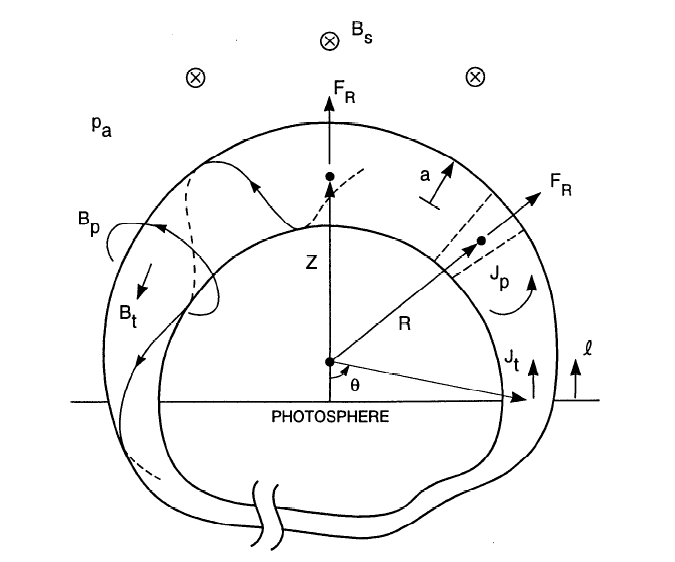
\includegraphics[scale=0.4, trim=0cm 1cm 0cm 1cm]{images/chen_model}
\caption[The toroidal instability CME model]{The flux rope model of \citet{chen1989}, used to to study the toroidal instability of a twisted flux system in the corona.}
\label{fig:chen_model}
\end{center}
\end{figure}
The equation of motion of the entire system is given by
\begin{equation}
M\frac{d^2Z}{dt^2} = \frac{I_t}{c^2R}\times\bigg[ \mathrm{ln}\bigg(\frac{8R}{a}\bigg) -1+ \frac{\xi_i}{2} + \frac{\beta_p}{2} -\frac{B^2_t}{B^2_{pa}}  -\frac{2RB_{\perp c}}{aB_{pa}} \bigg] - F_g - F_{drag}
\end{equation}
where $I_t$ is the toroidal current, $R$ is the flux rope major radius, $a$ is the rope minor radius, $\xi_i$ is internal inductance of the flux system, $B_t$ is the toroidal field, $B_{pa}$ is the poloidal field at $a$, $B_{\perp c}$ is the perpendicular component of the ambient coronal field, $F_g$ is the force due to gravity, $F_{drag}$ is the drag force, $M$ is the mass per unit length of the rope, and $Z$ is the rope axis height above the photosphere. The equation of motion shows that an increase in the toroidal current (or poloidal flux) contributes positively to the acceleration. The terms in the square brackets are each unitless and take into account the rope geometry, self-inductance and interplay between poloidal and toroidal flux. The first three terms in the square brackets are what give rise to the hoop-force. If the rope is mass loaded with a prominence, this can contribute to the rope's stability via the gravity term. The drag term only becomes an important contributor to rope dynamics later in the propagation, when the solar wind speed begins to increase i.e., at around 10$R_{\odot}$ \citep{sheeley1997}. The eruption is driven by flux-injection, which typically lasts for 4-8 hours, during which time the unstable system loses its equilibrium and begins to rise \citet{krall2001}.

It is significant the fluxrope is already established in the corona before eruption begins i.e., the rope formation is not addressed in the model and it is not a consequence of eruption. Hence magnetic reconnection is not a necessary aspect of the model and the eruption may proceed without employing resistive MHD. The model has been tested against observations and found to provide consistent result with the acceleration and jerk profiles of destabilized filaments during eruption \citep{schrijver2008}

%\subsection{Drag Models}\label{sec:23}
\section{Coronal Shocks and Plasma Emission}\label{sec:3}

\subsection{Alfv\'{e}n Speed in the Corona}
The speed at which perturbations travel in a magnetized plasma is the Alfv\'{e}n speed, given by
\begin{equation}
v_A = \frac{B_0}{\sqrt{\mu_0 \rho}}
\end{equation}
where $B_{0}$ is the unperturbed (equilibrium) magnetic field, $\mu_{0}$ is the magnetic permeability, and $\rho_{0}$ is the unperturbed mass density of the medium. This is a highly anisotropic wave driven by the restoring force of magnetic tension, with the inertia provided by the plasma mass density. Perturbations in the magnetic field, $B_{1}$, are transverse to the direction of $B_0$ and the group velocity always has a wave $\hat{k}$ vector parallel to the magnetic field direction. The quiet solar corona in the range of $1-3$\,$R_{\odot}$ has typical magnetic field strengths on the order of 1$-$100\,G\,=\,10$^{-2}-$10$^{-3}$\,T, and typical electron number densities of 10$^{6} -$10$^{9}$\,cm$^{-3}$\,=\,10$^{12}-$10$^{15}$\,m$^{-3}$, so for $B_0$=5 G and $n_e$=10$^{8}$\,cm$^{-3}$ the Alfv\'{e}n speed in the corona is $\sim$1000\,km$\cdot$s$^{-1}$. The variation in magnetic field and density in the corona, especially nearby an active region, $v_{A}$ may be on the order of 10$^{2}-$10$^{3}$\,km$\cdot$s$^{-1}$. If displacement components of the wave are perpendicular as well as parallel to the equilibrium magnetic field and non-zero perturbations in plasma thermal pressure and density occur, the result is a wave propagation known as a magnetoacoustic wave, such as the fast and slow mode MHD waves. However, given the corona is a low$-\beta$ plasma, magnetic perturbations are faster than thermal pressure ones, so the Alfv\'{e}n speed is a good estimate of plasma perturbation speeds in the corona.
\begin{figure}
\begin{center}
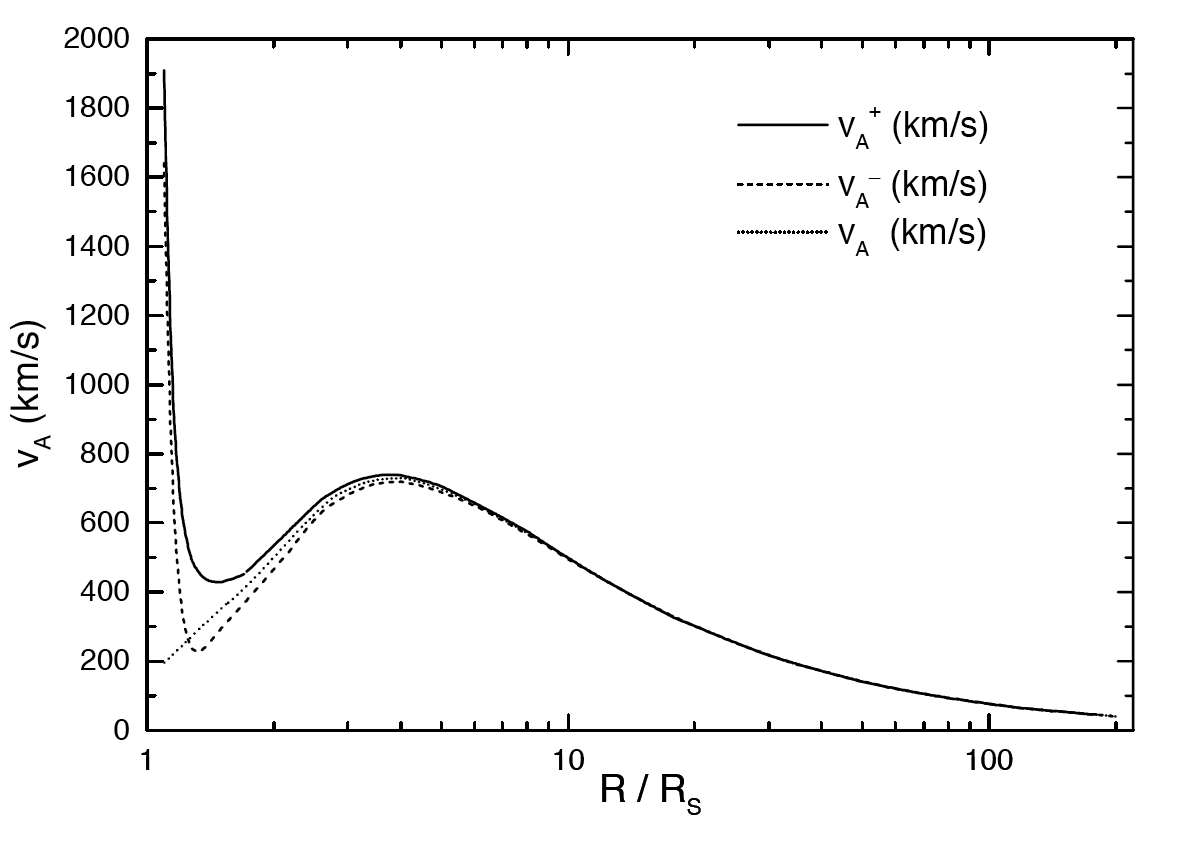
\includegraphics[scale=0.25, trim=0cm 2cm 0cm 2cm]{alfven_speed.png}
\caption[Model of the Aflv\'{e}n speed as a function of height in the corona]{Alfv\'{e}n speed of the corona as a function of heliocentric distance. The dotted line is the quite sun, with only the Sun's global dipole field. The solid line is the Alfv\'{e}n speed calculated from a combination of te global dipole field and a smaller active region dipole field oriented parallel to the global dipole. The dashed line is the the speed when the active region dipole is anti-parallel to the global field. The two profiles from the active region show a distinct minimum in the coronal Alfv\'{e}n speed at $\sim1.5\,R_{\odot}$}
\label{fig:alfven_speed}
\end{center}
\end{figure}
Mann et al. produced a 1D model of the variation of Alv\'{e}n speeds in the quiet and active region corona as a function of height Figure. Warmuth then improved this to a 2D model. It shows that CMEs are well capable of producing plasma hocks in the corona, since they may travel far in excess of the Alfv\'{e}n speed. The theory of plasma shocks and the resulting effects of particle acceleration and plasma emission are discussed in the following sections.


\subsection{MHD Shocks}\label{sec:mhd_shocks}

For acoustic shock waves there are a number of conservation equations that quantify the strength of a shock by relating the upstream gas pressure, density, flow speed, and temperature to their downstream counterparts. Such conservation equations are known as the jump conditions and the shock is considered a surface at which the fluid properties change discontinuously. The shock thickness is usually of the order of a few mean free paths of the particles in the gas, in such a case the processes in the shock surface itself are inconsequential and the relationship between upstream and downstream parameters provide a sufficient description of the shock. 

When the gas is ionized and a magnetic field is present, the jump conditions must be modified to take into account the magnetic pressure and the field orientation with respect to the flow velocity and shock normal $\hat{n}$ (unit vector normal to the shock plane). In the general case of oblique shock waves where the magnetic field direction has some arbitrary angle with respect to shock normal we may derive a set of conservation equations for the frame of the shock wave. 
\begin{figure}[h!]
\begin{center}
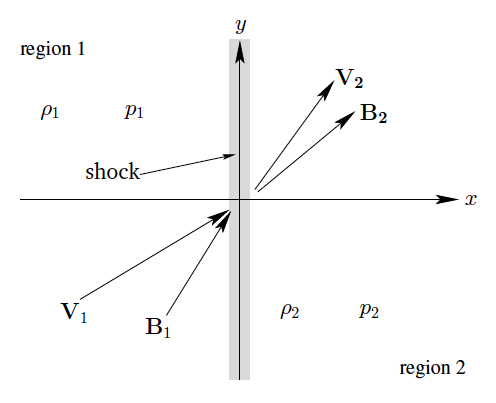
\includegraphics[scale=0.5, angle=0]{images/shock_pic}
\caption[MHD shock framework]{Orientation of magnetic field and velocity field with respect to shock plane, in the rest frame of the shock. Shock normal in this case would be along the $-x$ direction i.e., into upstream region 1. \citep{fitz}}
\label{fig:shock_pic}
\end{center}
\end{figure}

The flow velocity $v$ and magnetic field $B$ are considered to be in the xy-plane. The appropriate conservation  equations are
\begin{subequations}
\begin{align}
&[\rho v_{x}]=0 \\
&[\rho v_{x}^2+p+\dfrac{B_{y}^2}{2\mu}]=0 \\
&[\rho v_{x}v_{y} - \dfrac{B_{x}B_{y}}{\mu}]=0 \\
&[\dfrac{1}{2}v^2 + \dfrac{\gamma p}{(\gamma-1) \rho}+\dfrac{ B_{y}(v_{x}B_{y} - v_{y}B_{x})}{\mu \rho v_{x}} ]=0 \\
&[B_{x}]=0 \\
&[v_{x}B_{y} - v_{y}B_{x}]=0 
\end{align}
\end{subequations}
These are the general MHD shock jump conditions where $v$ is the fluid velocity and $B$ is the magnetic field (with their corresponding components $\textquoteleft$x' or $\textquoteleft$y'), $\rho$ is the mass density, $p$ is the thermal pressure, and $\gamma$ is the ratio of specific heats (or the polytropic index). The meaning of the square brackets is $[F]\equiv F_{1}-F_{2}$, for any quantity F, and the $1$ or $2$ subscripts represent upstream or downstream values of each quantity F, respectively. These set of jump conditions differ only from the purely acoustic ones due the presence of the magnetic field. For example, taking (4a), (4b), and (4d) and setting $B_{x}=B_{y}=0$ we obtain the jump conditions for a neutral gas. Each conservation equation has a specific meaning; 
\begin{itemize}
\item (4a) is a mass conservation equation whereby the mass flux entering the shock must equal the mass flux leaving. It has units of kg\,m$^{-2}$\,s$^{-1}$.
\item (4b) indicates that if mass flux $\rho_{1} v_{x,1}$ enters the shock with momentum $(\rho_{1} v_{x,1})v_{x,1}$ it leaves the shock with momentum $(\rho_{1} v_{x,1})v_{x,2}$, the difference being equal to the the changing force per unit area across the shock. In this case both thermal and magnetic pressures contribute to change in momentum flux. (4c) implies the same process but relates the $x$ and $y$ components of the $v$ and $B$ vector fields. Both equations have units of momentum flux $\equiv$ (kg\,m$^{-2}$\,s$^{-1}$)(m\,s$^{-1}$) = (kg\,m\,s$^{-2}$m$^{-2}$) = N\,m$^{-2}\equiv$ pressure.
\item (4c) is an energy conservation term, accounting for the rate at which gas and magnetic pressure do work per unit area at the shock and equates this to the growth (or loss) in internal energy and kinetic energy across the shock. All components of magnetic field pressure are taken into in the last term on the left of the equation. All quantities are in units of J$\cdot$kg$^{-1}$.
\item (4d) simply states that the x component of the magnetic field i.e., the component of the field that is (anti-)parallel to the shock normal $\hat{n}$ is unaffected by the shock transition. 
\item (4f) relates the orientations of the upstream and downstream magnetic field to the flow speed tangential and perpendicular to the shock normal. Magnetic field orientation and hence the distribution of low speed amongst the velocity components largely depends on the whether the shock is slow-mode, intermediate, or fast mode. The equation has units of T$\cdot$m$\cdot$s$^{-1}$ = V$\cdot$m$^{-1}\equiv$ electric field.
\end{itemize}

4(a-f) are the general case of the jump conditions across an MHD shock, they are usually known as the MHD Rankine-Hugoniot (RH) equations. Their generality make the solution of the six unknowns from the six equations quite complicated. However the extreme cases of parallel and perpendicular shocks provide very useful and simplified expressions. It can be shown that parallel shocks i.e., $\hat{v}\parallel\hat{B}\parallel\hat{n}$ reduces to the jump conditions of a hydrodynamic shock in a neutral gas (here parallel and anti-parallel are used synonymously). The more interesting case when considering radiating shockwaves in the low solar corona is the perpendicular (or quasi-perpendicular) MHD shock, in this case the flow speed is parallel to the shock normal, and the magnetic field is perpendicular (or at a high angle) to it i.e., $\hat{v}\,\|\,\hat{n}$ and $\hat{B}\perp\hat{n}$. As will be shown it is this special case of quasi-perpendicular shocks that lead to efficient shock drift particle acceleration, a necessary precursor to the generation of radio emission at a coronal shockwave. 

In the case of fully $\perp$ shocks there is no need for the decomposition of the magnetic and velocity vector fields, meaning the $x$ and $y$ subscripts on 4(a) and 4(b) can be dropped. 4(c) is an obsolete jump condition, likewise for 4(e) since no $B_x$ field exists. We can also rid the $B_{x}B_{y}$ terms from the last quotient in the energy conservation 4(d) --replacing it simply with $B^{2}/2\mu\rho$. 4(f) reduces to a simpler form of $[Bv]=0$. Such a reduction in the generalized jump conditions allows us to express the upstream and downstream plasma properties in terms of the shock compression ratio $\chi=\dfrac{\rho_{2}}{\rho_{1}}$ as well as the upstream sonic Mach number $M_{1}=\dfrac{v_{1}}{c_{1}}$ \citep{priest2000} e.g.,
\begin{subequations}
\begin{align}
&\dfrac{v_{2}}{v_{1}}=\frac{1}{\chi} \\
&\dfrac{B_{2}}{B_{1}}=\chi \\
&\dfrac{p_{2}}{p{1}}=\gamma M_{1}^2\bigg(1-\frac{1}{\chi}\bigg) - \frac{1-\chi^2}{\beta_{1}}
\end{align}
\end{subequations}
where $\beta_{1}=2\mu p/B_{1}^2$ is the upstream plasma beta parameter. The exact value of the compression ratio may be obtained by using 4(b) to eliminate $p$ from the energy flux equation 4(d) and incorporating 4(a,c,e,f) (and a lot of algebra) a quadratic for $\chi$ may be obtained
\begin{equation}
2(2-\gamma)\chi^{2}+[2\beta_{1}+(\gamma-1)\beta_{1}M_{1}^2+2]\gamma\chi - \gamma(\gamma+1)\beta_{1}M_{1}^2=0
\end{equation}
%where $M_{1}$ is the upstream sonic Mach number, $\beta_{1}$ is the upstream beta parameter and, and $\gamma$ is the ploytropic index. 
Equation (6) has one positive real root such that 
\begin{equation}
1< \chi < \frac{\gamma+1}{\gamma-1}
\label{eqn:compression}
\end{equation}
Using a ploytropic index of $\gamma=5/3$ (monatomic) means the shock compression can be no more than a factor of 4. Another extremely important fact arising from this is that magnetic compression can also be no greater than 4 i.e., from equation 4(b) $B_{2}/B_{1}=\chi$. $\chi<4$ has consequences for the shock drift acceleration mechanism and provides an upper limit to the particle energy gain.

\subsection{Shock Particle Acceleration}\label{sec:30}

The framework of shock particle acceleration for solar type II radio bursts is called the shock drift acceleration (SDA) mechanism \citep{holman1983}. The mechanism involves a gyrating particle encountering the magnetic gradient caused by the shock, resulting in a guide center drift and an energy gain due to the presence of a convective electric field at the shock. 

There are two important frames of reference through which SDA is studied. In the rest frame of the shock, known as the \textquoteleft normal incidence frame' (NIF), the upstream plasma has velocity $\mathbf{u}_1$ along the normal $\hat{n}$ to the shock front. The upstream magnetic field $\mathbf{B}_1$ creates an angle $\theta_{Bn}$ with the shock normal $\hat{n}$, and the downstream counterparts have values $\mathbf{u}_2$ and $\mathbf{B}_2$, Figure~\ref{fig:nif_dht}(left). 

\begin{figure}[!t] 
\begin{center}
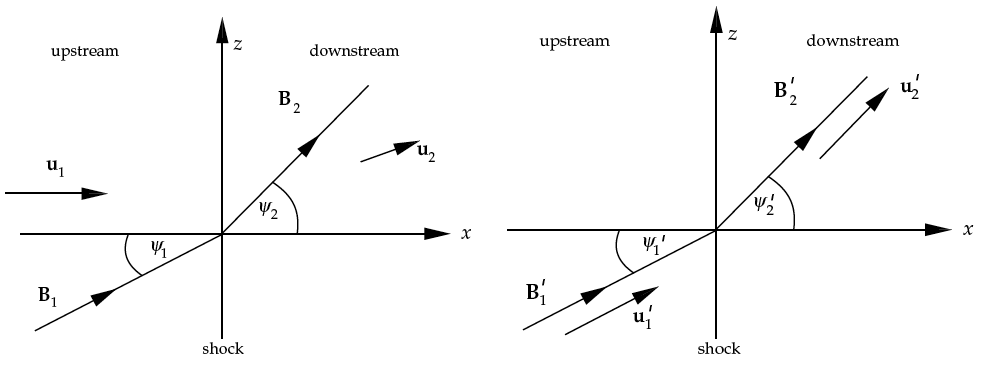
\includegraphics[scale=0.45]{nif_dht}
\caption[Normal incidence and de Hoffman-Teller reference frames]{(Left) Normal incidence frame (NIF) where the shock is at rest and the upstream plamsa approaches the shock head-on at velocity $\mathbf{u}_1$. The magnetic field makes some arbitrary angle $\theta_{Bn}$ with the shock normal. (Right) Transformation to a de Hoffman-Teller frame ensures that the plasma velocity and magnetic field are in the same direction on both sides of the shock \citep{ball2001}.}
\label{fig:nif_dht}
\end{center}
\end{figure}

Due to the motion of the plasma across the magnetic field, there is a convective electric field given by $\mathbf{E} = \mathbf{v}\times \mathbf{B}$, which causes a drift of the particles with speed $\mathbf{v}_E = \mathbf{E}\times \mathbf{B}/B^2$. The kinematics of the particle in the shock drift acceleration mechanism are best treated in a frame where there the convective electric field vanishes such that $\mathbf{E} = |\mathbf{v}\times \mathbf{B}|=v_x B_y - v_yB_x = 0$. The frame where this criterion is fulfilled is known as the de Hoffmann-Teller frame (dHTf) \citep{dehoffmann1950} and has a frame velocity with respect to the NIF frame given by. 
\begin{equation}
v_{HT} = v_y = u_1\mathrm{tan}\theta_{Bn}
\end{equation}
This frame guarantees the plasma motion is in the same direction as the magnetic field on both sides of the shock. Given the absence of any electric fields in this frame, the particle motions may be treated as having a conserved magnetic moment \citep{ball2001}
\begin{equation}
\mu = \frac{mv^2_{1\perp}}{B_1} = \frac{mv^2_{2\perp}}{B_2} = \mathrm{const}
\label{eqn:ad_in}
\end{equation}
where the subscripts [1,2] represent pre an post-encounter shock values respectively. In the dHTf, the conservation of the magnetic moment may be used to derive the particle kinematics given either reflection or transmission though the shock. Rearrangement of equation \label{eqn:ad_in} shows that particles with a pitch angle fulfilling the relationship
\begin{equation}
\alpha > \alpha_c~~~~\mathrm{where}~~~~\mathrm{sin}^2\alpha_c = \frac{B_1}{B_2}
\end{equation}
will be reflected at the shock. This pitch angle $\alpha_c$ defines a \textquoteleft loss-cone' in velocity space $f(v_{\perp}, v_{||})$, whereby any particle within the cone (large $v_{||}$) will be lost downstream, while particles outside the loss cone will be reflected at the shock. This is known as a \textquoteleft magnetic mirroring', a process that shocks are known to exhibit \citep{feldman1983}. Inside the dHT reference frame, the particles energy (whether reflected or transmitted) is completely conserved and there is no energy gain. Conceptually, the best way to see where the acceleration takes place is in the normal indcidence frame (NIF).

In the NIF, the particles gyrate about the upstream magnetic field $\mathbf{B}_1$, while there is a convective electric causes a small drift of magnitude $\mathbf{v}_E = \mathbf{E}\times \mathbf{B}/B^2$ towards the shock. If the particle speed is much greater than the shock speed $v>>u$, the particle undergoes many Larmor gyrations while in contact with the shock. The difference between the Larmor radius of the orbit ahead of and behind the shock front (due to the increased downstream magnetic field) will cause the particle to drift parallel to the shock surface \citep{ball2001, toptychin1980}, Figure~\ref{fig:sda}. This is equivalent to a \textquoteleft grad-B' drift in an inhomogeneous magnetic field. This drift allows a charged particle to move parallel to the convective electric field, allowing the E-field to do positive work on the particle and produce an energy increase. Overall, a grad-B drift at the shock surface gives the particle a component of velocity that may interact with the convective electric field, hence the process is known as \textquoteleft drift-acceleration'.

\begin{figure}[!t] 
\begin{center}
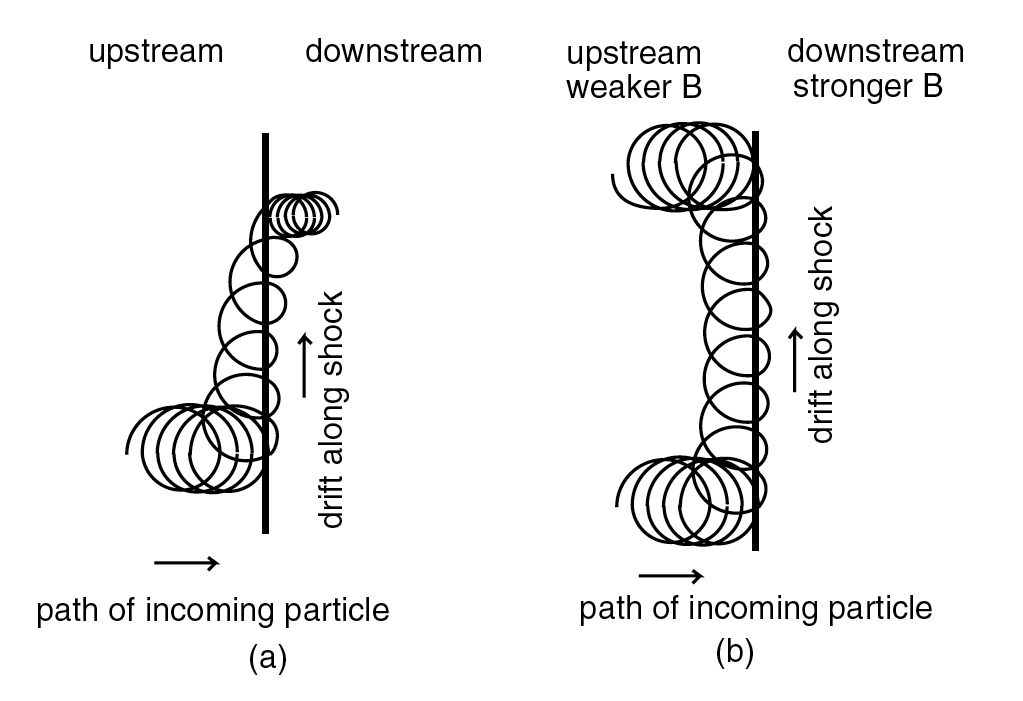
\includegraphics[scale=0.3]{sda_original}
\caption[Shock drift acceleration]{Particle drift paths due during both a transmitted (a) and reflected (b) motion. The increased magnetic field in the downstream region caused a drift along the surface. This drift occurs in the presence of a convective electric field (which will have a component parallel to the drift), allowing the field to do work on the particle and hence increase its energy \citep{ball2001}.}
\label{fig:sda}
\end{center}
\end{figure}

While the energy gain is most apparent in the NIF frame, particle reflection and transmission is best handled mathematically in the dHT frame. Hence firstly, the magnetic mirroring process is described in dHT, while the post-encounter speed and energy gain are then obtained by converting back to the rest frame of the upstream plasma (NIF). Reference has shown that the particle energy gain upon reflection from the shock is given by 

\begin{equation}
\frac{E_r}{E_i} = \frac{1+\sqrt{1-B_1/B_2}}{1-\sqrt{1-B_1/B_2}}
%v^r_{||} = 2u_1\mathrm{sec}\theta_1 - v^i_{||}
\end{equation}
The energy gain is limited to the magnetic field strength jump across the shock, and since this field strength is limited by equation~\ref{eqn:compression}, the energy gain is limited to a factor of 13.93 \citep{ball2001}. A similar treatment may also give the reflected velocity in terms of the incident velocity \citep{holman1983}
\begin{equation}
v^r_{||} = 2u_1\mathrm{sec}\theta_1 - v^i_{||}
\end{equation}
shock drift acceleration has been used to explain the presence of $1-100$\,keV electron at Earth's magnetospheric bow shock \citep{wu1984}, in the context of radio bursts have used it to explain the acceleration of electrons during type II and herringbone bursts \citep{holman1983, mann2005, schmidt2012b}
More sophisticated models involve multiple reflections at the shock that increase the energy gain each time, thereby producing energies that are observed in the vicinity of shocks. This multiple reflection process plays an important role in some theoretical treatments of herringbone emission; we will return to this point in Chapter 5.



\subsection{Wave-Particle Interaction}\label{sec:wave_particle}

%Distributions of particles in a plasma can give rise to resonances in various wave modes. In general we may relate a particle distribution function in velocity space $f(v_{\|})$ with a distribution function of wave modes in wave-number or $\textquoteleft\mathbf{k}$-space' $N(\mathbf{k})$
%\begin{equation}
%\frac{\partial N(\mathbf{k})}{\partial t}+v_{g}(\mathbf{k})\frac{\partial N(\mathbf{k})}{\partial r} = \Gamma(\mathbf{k},f(v_{\|}))N(\mathbf{k})
%-\Gamma_{coll}(\mathbf{k}) N(\mathbf{k})
%\end{equation}
%where the lefthand side takes the form of a Lagrangian derivative with group speed $v_g$, $\Gamma$ represents a wave growth term given the distribution function $f(v_{\|})$, and $\Gamma_{coll}$ is a term taking into account collisional damping of the wave \citep{aschbook}.

The treatment of the interaction of particles and waves in a plasma is in determining what the oscillatory response of a plasma is to a velocity distribution function \citep{inan2011}. In order to see how the distribution function effects wave growth we start with an equilibrium distribution $f_0$ and impose a perturbation $f_1(\mathbf{r}, \mathbf{v}, t)$, so that the total distribution function is $f(\mathbf{r}, \mathbf{v}, t) = f_0 +f_1(\mathbf{r}, \mathbf{v}, t)$.  The perturbation quantities will take the form $e^{i(\omega t + \mathbf{k}r)}$ i.e., perturbation quantities that are periodic in space and time with eave number $\mathbf{k}$ and angular frequency $\omega$.

To see how $f(\mathbf{r}, \mathbf{v}, t)$ evolves in time we insert it into the Vlasov equation and linearize, ignoring any terms higher than second order
\begin{equation}
\frac{\partial f_1}{\partial t} + (\mathbf{v}\cdot \nabla)f_1 +\frac{q_e}{m_e}(\mathbf{E} + \mathbf{v}\times \mathbf{B})\cdot\nabla_vf_0=0
\end{equation}
%Assuming an isotropic $f_0$ it can be shown that $(\mathbf{v}\times \mathbf{B})\cdot\nabla_vf_0=0$, and 
Using Poisson's equation (Maxwell first equation) and replacing the time and space derivatives with their oscillatory operators ($\partial/\partial t \rightarrow -i\omega$, $\nabla \rightarrow i\mathbf{k}$), the perturbed Vlasov equation may be rearranged to give
\begin{equation}
f_1=\frac{q_e}{m_e}\frac{j}{\omega-\mathbf{k\cdot v}}\mathbf{E}\cdot\nabla_vf_0
\label{eqn:f_pert}
\end{equation}
This equation relates the perturbed quantity $f_1$ to the unperturbed distribution function and the electric field. The most important aspect of this equation is the $\omega-\mathbf{k\cdot v}$ term in the denominator, implying the possibility of resonance. Now, integrating both sides of \ref{eqn:f_pert} over all velocity space and again using Poisson's equation results in
%using (19) the general form of the dispersion relation of the oscillations $(\omega,\mathbf{k})$ in perturbations $f_1$ and $E$ is derived
\begin{equation}
1+\frac{q_e}{\epsilon_0m_e}\frac{1}{k^2}\mathbf{k}\cdot\int_v\frac{\nabla_v f_0}{\omega-\mathbf{k\cdot v}}d^3v=0
\label{eqn:dispersion}
\end{equation}
Any electrostatic normal mode oscillations satisfy this relationship and integrating over all velocity space will result in a dispersion relation for the oscillations of the plasma property $f_1$. The equation effectively gives the oscillatory response $\omega = g(\mathbf{k})$ of the perturbation $f_1$ of the plasma, given a particular velocity distribution function $f_0$. For example, a cold plasma distribution function where $f_0 = N_0\delta(\mathbf{v})$, where $\delta$ is a dirac-delta, in equation~\ref{eqn:dispersion} will result in a dispersion relation of
\begin{equation}
1 - \frac{N_0q_e^2}{\epsilon_0 m_e \omega^2} = 0 
\end{equation}
The perturbed Vlasov equation with a cold plasma model (no thermal motions) produces the expression for a plasma oscillation. The integral over velocity space in this case can be performed because the delta function guarantees that there is no velocity with the property of $v = \frac{\omega}{\mathbf{k}}$. If this were to be fulfilled, there is the possibility of resonances equation~\ref{eqn:dispersion} i.e., the integral is non-trivial as $v \rightarrow \frac{\omega}{k}$. This states that if there are electrons in the particle distribution function that match the phase speed of oscillations in the plasma then the integral will have a singularity or 'pole'. To avoid the singularity producing unphysical results, the integration is performed in complex space using a method called contour integration \citep{melrose1989}. The use of contour integration means there will be complex solutions of the dispersion relation of the form $\omega = \omega_r + i\gamma$.
The real part of the solution applies as normal where the integral is well behaved, far from the singularity. However, integration over the singularity necessitates a complex solution (from the contour integration), hence the $\omega$ consists of both real and imaginary parts.
The complex $i\gamma$ means that a time dependency of the periodic solutions to the perturbations $f_1$ will be 
\begin{equation}
e^{j\omega t}=e^{(i[\omega_r + i\gamma])}=e^{i\omega_rt}e^{-\gamma t}
\end{equation}
This solution is a damped wave with damping factor $\gamma$, meaning the solution to equation~\ref{eqn:dispersion} in the region $v \sim \omega/k$ provides a wave decay term. These are the essential elements of Landau damping e.g., if the phase speed of the waves in a plasma match the speed of electrons in the distribution function then those waves will experience a damping. However, the damping term is dependent on the negative of the velocity space gradient at $v=\frac{\omega}{k}$ \citep{melrose1989}
\begin{equation}
\gamma \sim -\nabla_v f_0|_{v=\frac{\omega}{k}}
\end{equation}
If there are a group of electrons that have the same speed of a particular wave in the plasma they may exchange energy with this wave efficiently. If there is a negative gradient on the velocity distribution at $v=\frac{\omega}{k}$, this will lead to wave damping. However, a positive gradient in the velocity distribution will result in $\gamma <0$ and a wave growth term that increases exponentially. Effectively, %if a group of electrons is promoted to a speed that matches the phase speed of Langmuir waves in the plasma, and their velocity space gradient at the phase speed is positive, then Langmuir waves will grow exponential. This group of electrons is called a bump-on-tail, since it is described by a Gaussian bump on the high velocity tail of a Maxwell distribution function. The growth of Langmuir waves in a resonant response to this beam is called the bump-on-tail instability.
a group of electrons is promoted to a velocity range that closely matches the phase speed of some type of waves in a medium $v \sim \omega/k$. In such a speed range the integrand of (equation) approaches the point at which there is a singularity in the solution. Such a point necessitates a complex solution to the integral, thus providing an imaginary part to the dispersion relation that gives an $e^{-\gamma t}$ term. If the promotion of electrons to a range $v \sim \omega/k$ is combined with a positive gradient of the distribution function in this velocity range, it results in $\gamma < 0$ and $e^{-\gamma t}>0$, leading to wave growth. This is why $v - \omega/k=0$
is known as the resonance condition \citep{melrose1989}. Since electron beams in the corona match the phase speed of Langmuir waves, the beam results in the generation of Langmuir waves. This group of electrons in the beam is called a bump-on-tail, since it is described by a Gaussian bump on the high velocity tail of a Maxwell-Boltzmann velocity distribution function (Figure~\ref{fig:bot}). 
\begin{figure}[!t] 
\begin{center}
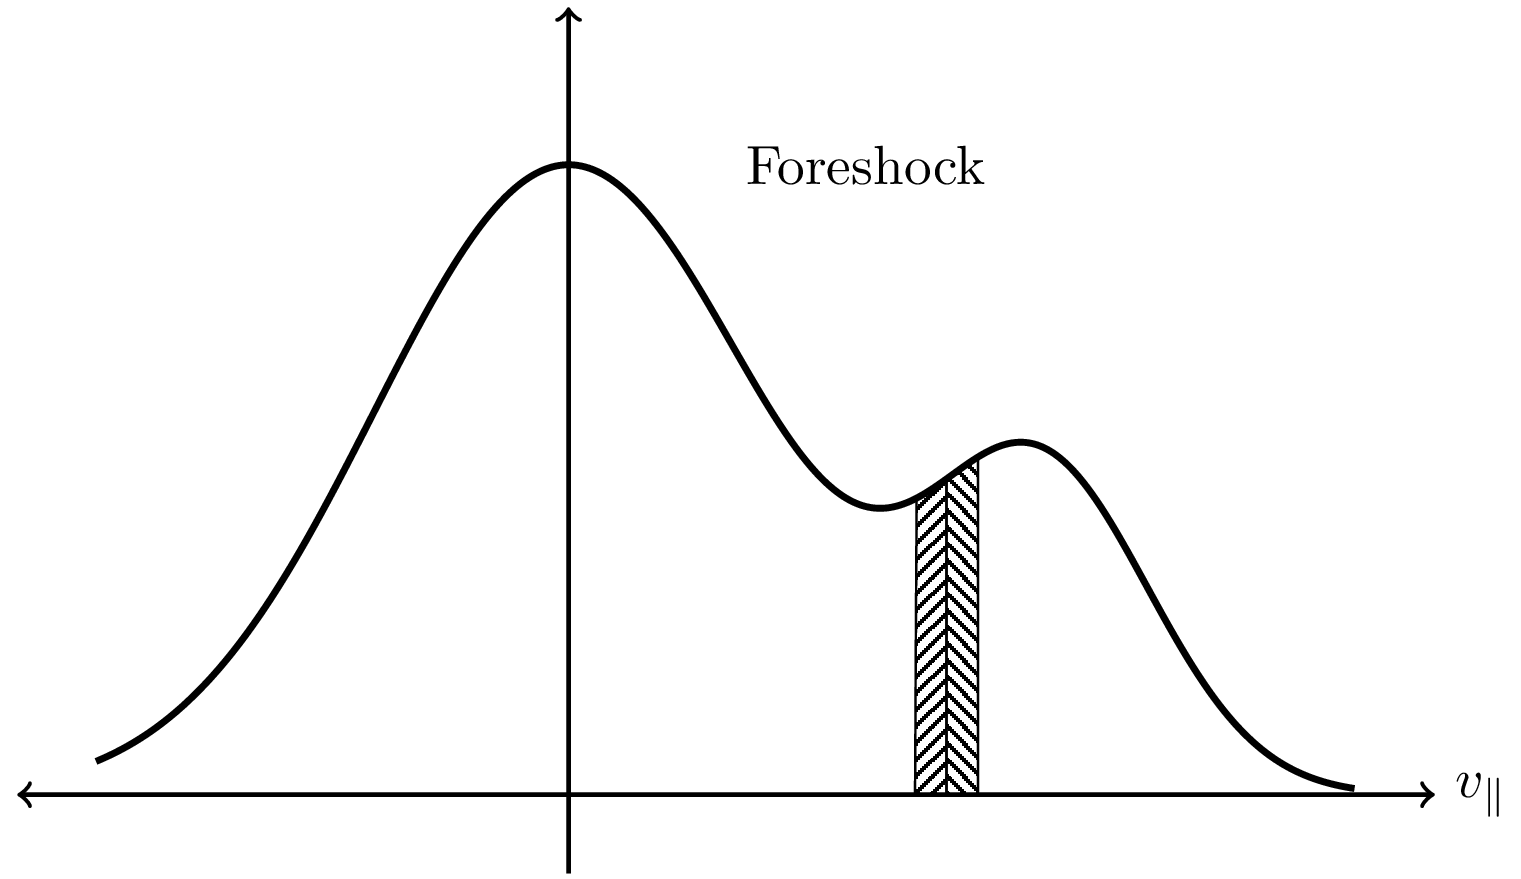
\includegraphics[scale=0.2]{bump_on_tail}
\caption[Shock drift acceleration]{Maxwell-Boltzmann velocity distribution with a Guassian `bump-on-tail' representing the beam. The shaded region are those electrons that will produce a bump-on-tail instability due to the presence of a positive slope in the distribution function.}
\label{fig:bot}
\end{center}
\end{figure}
The growth of Langmuir waves in a resonant response to this beam is called the bump-on-tail instability. Once these Langmuir waves are generated they may undergo decay or coalescence with other waves to produce electromagnetic radiation. 

%\begin{figure}[!t]
%\begin{center}
%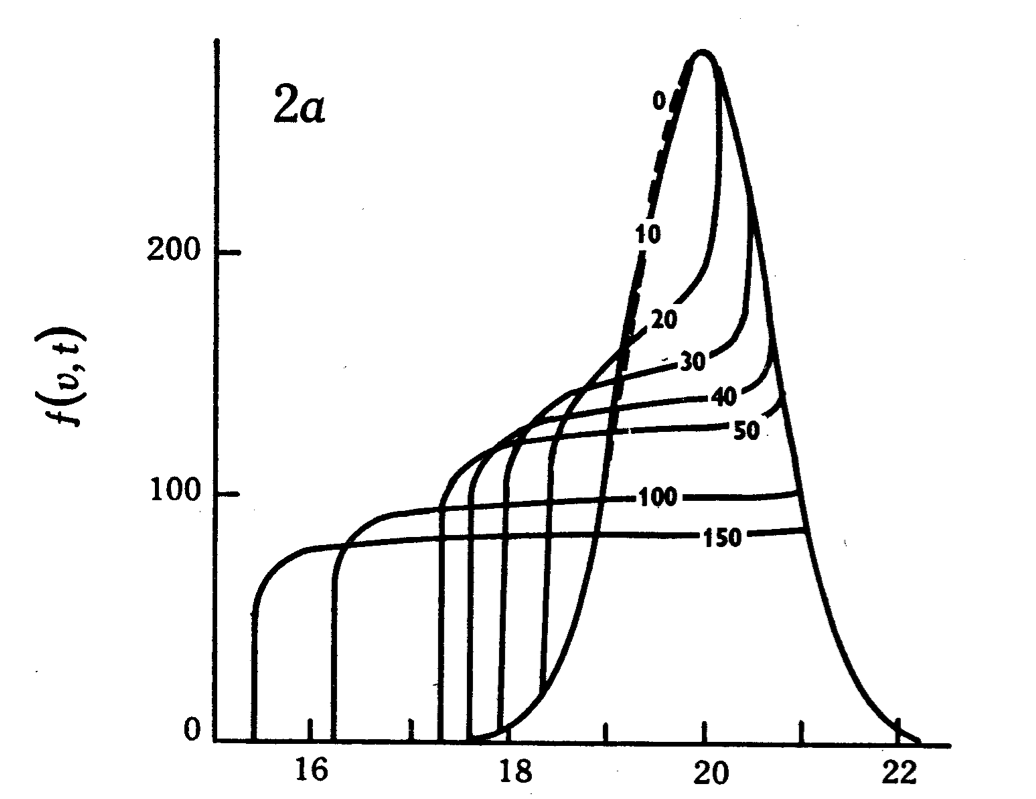
\includegraphics[scale=0.35, trim = 4cm 0cm 0cm 0cm]{images/Grognard1975}
%\end{center}
%\end{figure}


\subsection{Three-Wave Interaction and Plasma Emission}\label{sec:three_wave}

Once the Langmuir waves are produced from the bump-on-tail instability a number of wave interaction processes occur in order to bring about plasma emission. This involves the interaction of various wave modes in the plasma described by a mathematical formalism called the three-wave interaction \citep{robinson1993, robinson1994}. In this process three wave modes in a plasma M, P, and Q are described by their distribution functions in a wave-number space ($k$-space). the distribution functions are given by $N_M(k_M)$, $N_P(k_P)$, $N_Q(k_Q)$, where the $N$ describe the occupation number of wave quanta between $k$ and $k+dk$ in the wave-number space. Waves in P and Q mode may interact to such that wave quanta are removed from the P and Q k-space and added to the M k-space. This is essentially an emission of an energy packet from the P and Q -space to the M k-space. The rate of change of occupation numbers in the three k-spaces are given by
\begin{eqnarray}
\frac{dN_M(\mathbf{k}_M)}{dt} = -\int \frac{d^3\mathbf{k}_P}{(2\pi)^3}\int \frac{d^3\mathbf{k}_Q}{(2\pi)^3}g(\mathbf{k}_M, \mathbf{k}_P, \mathbf{k}_Q) \\
%
\frac{dN_P(\mathbf{k}_P)}{dt} = -\int \frac{d^3\mathbf{k}_M}{(2\pi)^3}\int \frac{d^3\mathbf{k}_Q}{(2\pi)^3}g(\mathbf{k}_M, \mathbf{k}_P, \mathbf{k}_Q) \\
%
\frac{dN_Q(\mathbf{k}_Q)}{dt} = -\int \frac{d^3\mathbf{k}_M}{(2\pi)^3}\int \frac{d^3\mathbf{k}_P}{(2\pi)^3}g(\mathbf{k}_M, \mathbf{k}_P, \mathbf{k}_Q)
\end{eqnarray}
where $g(\bf{k}_M, \bf{k}_P, \bf{k}_Q)$ is an expression that incorporates a transition probability for wave quanta into and out of energy states in the various k-spaces \citep{robinson1994}. The transition probability of waves amongst states M, P and Q is given by \citep{melrose1986}
\begin{equation}
u_{MPQ}(\mathbf{k}_M, \mathbf{k}_P, \mathbf{k}_Q)  \propto \delta(\omega_M - \omega_P - \omega_Q ) \delta^3(\mathbf{k}_M - \mathbf{k}_P - \mathbf{k}_Q )
\end{equation}
where the $\omega$ are the frequency of the corresponding wave and and $\delta$ are delta functions. This is analogous to transition probabilities given by the Einstein coefficients for transferring energy packets from and atomic state to a photon state (photon emission) i.e., whereas the Einstein coefficients are used in atom-wave (atom-photon) energy exchanges, $u_{MPQ}$ describes wave-wave energy exchanges. Given the presence of delta functions in the transition probability expression, we can see that an exchange of energy quanta amongst the wave modes can only occur when 
\begin{eqnarray}
\omega_M & = & \omega_P + \omega_Q \\
\mathbf{k}_M & = & \mathbf{k}_P + \mathbf{k}_Q
\end{eqnarray}
Hence for an a conversion wave modes in a plasma such as $M \rightarrow P + Q$ (a decay of mode M into P and Q), or it's reverse process $P + Q \rightarrow M $ (a coupling of P and Q to produce M) is described by equations (2.1) to (2.7). 

%\begin{multline}
%g(\mathbf{k}_M, \mathbf{k}_P, \mathbf{k}_Q) = u_{MPQ}(\mathbf{k}_M, \mathbf{k}_P, \mathbf{k}_Q)   [N_M(\mathbf{k_M}) N_P(\mathbf{k_P})  - \\ 
%N_P(\mathbf{k_P}) N_Q(\mathbf{k_Q})   +N_Q(\mathbf{k_Q}) N_M(\mathbf{k_M})  ]
%\end{multline}
%where $u_{MPQ}(\bf{k}_M, \bf{k}_P, \bf{k}_Q) $ is the transition probability from states in P and Q  to M, for example \citep{melrose1986}.  The transition probability is given by

%where the $\omega$ are the frequency of the corresponding wave and and $\delta$ are delta functions. 
The production of plasma emission after a bump-on-tail instability has occurred requires a three wave interaction amongst a Langmuir wave $L$, ion acoustic wave $S$, and electromagnetic wave $T$. Fundamental emission during a radio burst occurs via a decay of Langmuir waves into an electromagnetic and ion sound wave
\begin{equation}
L \rightarrow T + S
\label{eqn:fund}
\end{equation}
while second harmonic first requires the decay $L\rightarrow L^{'} + S$, where $L^{'}$ is a product Langmuir wave propagating in the opposite direction to the first. This is followed by a coalescence of the original and product Langmuir waves
\begin{equation}
L + L^{'}\rightarrow T'
\label{eqn:harm}
\end{equation}
In the case of these three interacting waves then 
\begin{eqnarray}
\omega_T & = & \omega_L + \omega_S \\
\omega_{T^{'}} & = & \omega_L + \omega_{L^{'}}
\end{eqnarray}
where the relevant dispersion relations are 
\begin{eqnarray}
\omega_L = \omega_p + \frac{3v_{th}^2}{2\omega_p}k_L^2 \\
\omega_T = (\omega_p^2 +k_T^2c^2)^{1/2} \\
\omega_S = k_s\sqrt{\frac{\gamma k_B T_e}{m_i}}
\end{eqnarray}
where
\begin{equation}
\omega_p = \bigg(\frac{n_e e^2}{m_e \epsilon_0}\bigg)^\frac{1}{2}
\label{eqn:plasma_frequency}
\end{equation}
These equations imply that when a Langmuir wave decays to an electromagnetic wave and an ion sound wave (equation 2.58), the frequency of the electromagnetic wave will be equal to that of the Langmuir wave such that $\omega_T = \omega_L \approx \omega_p$. This is why plasma emission occurs at the local plasma frequency. Similarly the production of $T^{'}$ via equation (2.59) results in the first harmonic $\omega_T \approx 2\omega_p$. 
%!!!!!!!!!!!!!!!!!!!!!!!!!!!!!
%
%PROVE THE ABOVE MORE CLEARLY!!!!!!!!!!!!!!!!!!!!!!
%
%!!!!!!!!!!!!!!!!!!!!!!!!!!!!

In order to investigate the amount of energy emitted by the electromagnetic wave, elements of the three wave interaction theory need to be combined with what is known as stochastic growth theory \citep{robinson1993a}(SGT). Stochastic growth theory was first developed in response to a number of criticisms of the theory of a beam-driven Langmuir wave hypothesis of type III radio bursts first proposed by \citet{ginzburg1958}. It was pointed out that if the beam was to remain in instability continuously over space and time in the absence of saturation mechanism, then it would quickly lose all of its energy to the Langmuir waves and consequently the beam electrons would stop propagating after a short distance \citep{sturrock1964}. This is clearly not the case, since type III electrons are observed to propagate over distances of 1\,A.U or more. 
%Secondly, if the instability continues uninhibited the Langmuir wave with grow to levels far beyond what is observed \citep{smith1979}. 
%It was concluded that the beam cannot remain in a state of instability for the duration of its propagation. One suggestion to over come this was quasi-linear relaxation \citep{grognard1975}, as described above. However, this may not be enough to guarantee a lone lifetime of the beam. 
SGT overcomes this by describing an electron beam propagation in a state of marginal stability. The beam propagates in an inhomogeneous medium whereby it encounters pockets of localised density enhancement where it is unstable intermittently. As the beam propagates through this localised clump, it is unstable to the growth of Langmuir wave, giving up some of its energy to the wave, diminishing the beam slightly. Once it exits the clump it becomes stable again, allowing the beam to reform until it reaches another localised clump to give up some energy again. The Langmuir waves would then experience a growth at intermittent regions in space and time (which is actually observed \citep{lin1986}), while the beam would be unstable for only small fractions of its lifetime. Overall, the beam energy loss is on average low enough to allow its continued propagation, but instantaneous and finite enough to allow the growth of waves. 
%In this mechanism the Langmuir waves experience a a growth in energy that is a random (stochastic) walk through energy phase space \citep{robinson1992}.  The Langmuir wave send up with an energy distribution given by $P(E)\sim E^{-1}$ \citep{robinson1993a}.  
\begin{figure}[t!]
\begin{center}
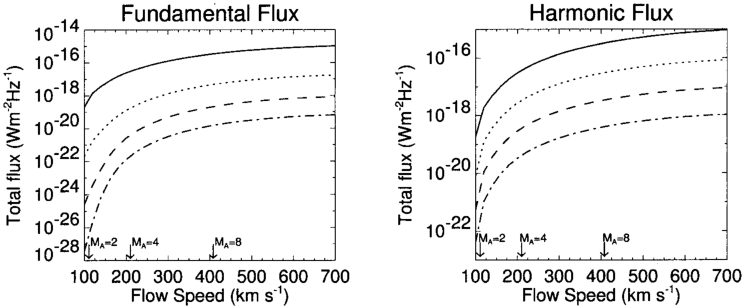
\includegraphics[scale=1.1, trim=0cm 0cm 0cm 0.5cm]{images/Cairns2003.pdf}
\caption[Theoretically predicted radio burst fluxes]{Theoretical flux of the fundamental and harmonic emission bands of a type II radio burst using three wave interaction and stochastic growth theory \citet{cairns2003}.}
\label{fig:cairns_emissivity}
\end{center}
\end{figure}
Combining elements of the stochastic growth model and the three-wave interaction process allows a calculation of the mount of energy that ends up in the electromagnetic waves, and consequently the volume emissivity of the emission \citep{robinson1993a, robinson1998}
\begin{equation}
j_M(r) \approx \frac{\Phi_M}{\Delta\Omega_M}\frac{n_b m_e v_b^3}{3l(r)}\frac{\Delta v_b}{v_b}
\end{equation}
here the $M$ stands for either fundamental $F$ or harmonic $H$ emission. $\Delta\Omega_M$ is the solid angle over which the  emission is spread, $n_b$ is the electron beam number density, $v_b$ is the beam speed, $l(r)$ is the distance from emission point to observer, $\Delta v_b$ is the width of the beam in velocity space. $\Phi_M$ are known as the conversion efficiencies and are different for fundamental and harmonic emission, see Appendix X.

These expressions have been used to simulate radio burst flux resulting in $\sim10^{-17}$\,W\,m$^{-2}$\,Hz$^{-1}$, which have been compared to type II and III radio bursts \citep{schmidt2012, knock2001}. \citet{knock2003} and \citet{cairns2003} used the theory to predict interplanetary type II burst flux as a function of a variety of shock parameters e.g., shocks speed Fig.~\ref{fig:cairns_emissivity}.

The theory outlined in section~\ref{sec:mhd_shocks} -- \ref{sec:three_wave} was employed in a model developed by \citet{schmidt2012b}, completely describing the generation of radio bursts from CME driven shocks. It involves the eruption of a flux rope into a background corona, the driving of a shock as described by the MHD Rankine-Hugoniot relations, the generation of electron beams via SDA, the growth of the bump-on-tail instability, and the generation of electromagnetic emission via the three-wave process and stochastic growth theory. The model finds that that radio emission is generated on the expanding flanks of a CME. The model also shows that when the shock is rippled, there will be spatially intermittent regions of electron beam generation, which could be possible explanation of herringbone emission (Figure~\ref{fig:herbone_model}).
% as shown in Figure~\ref{fig:schmidt_model}
%\begin{figure}[t!]
%\begin{center}
%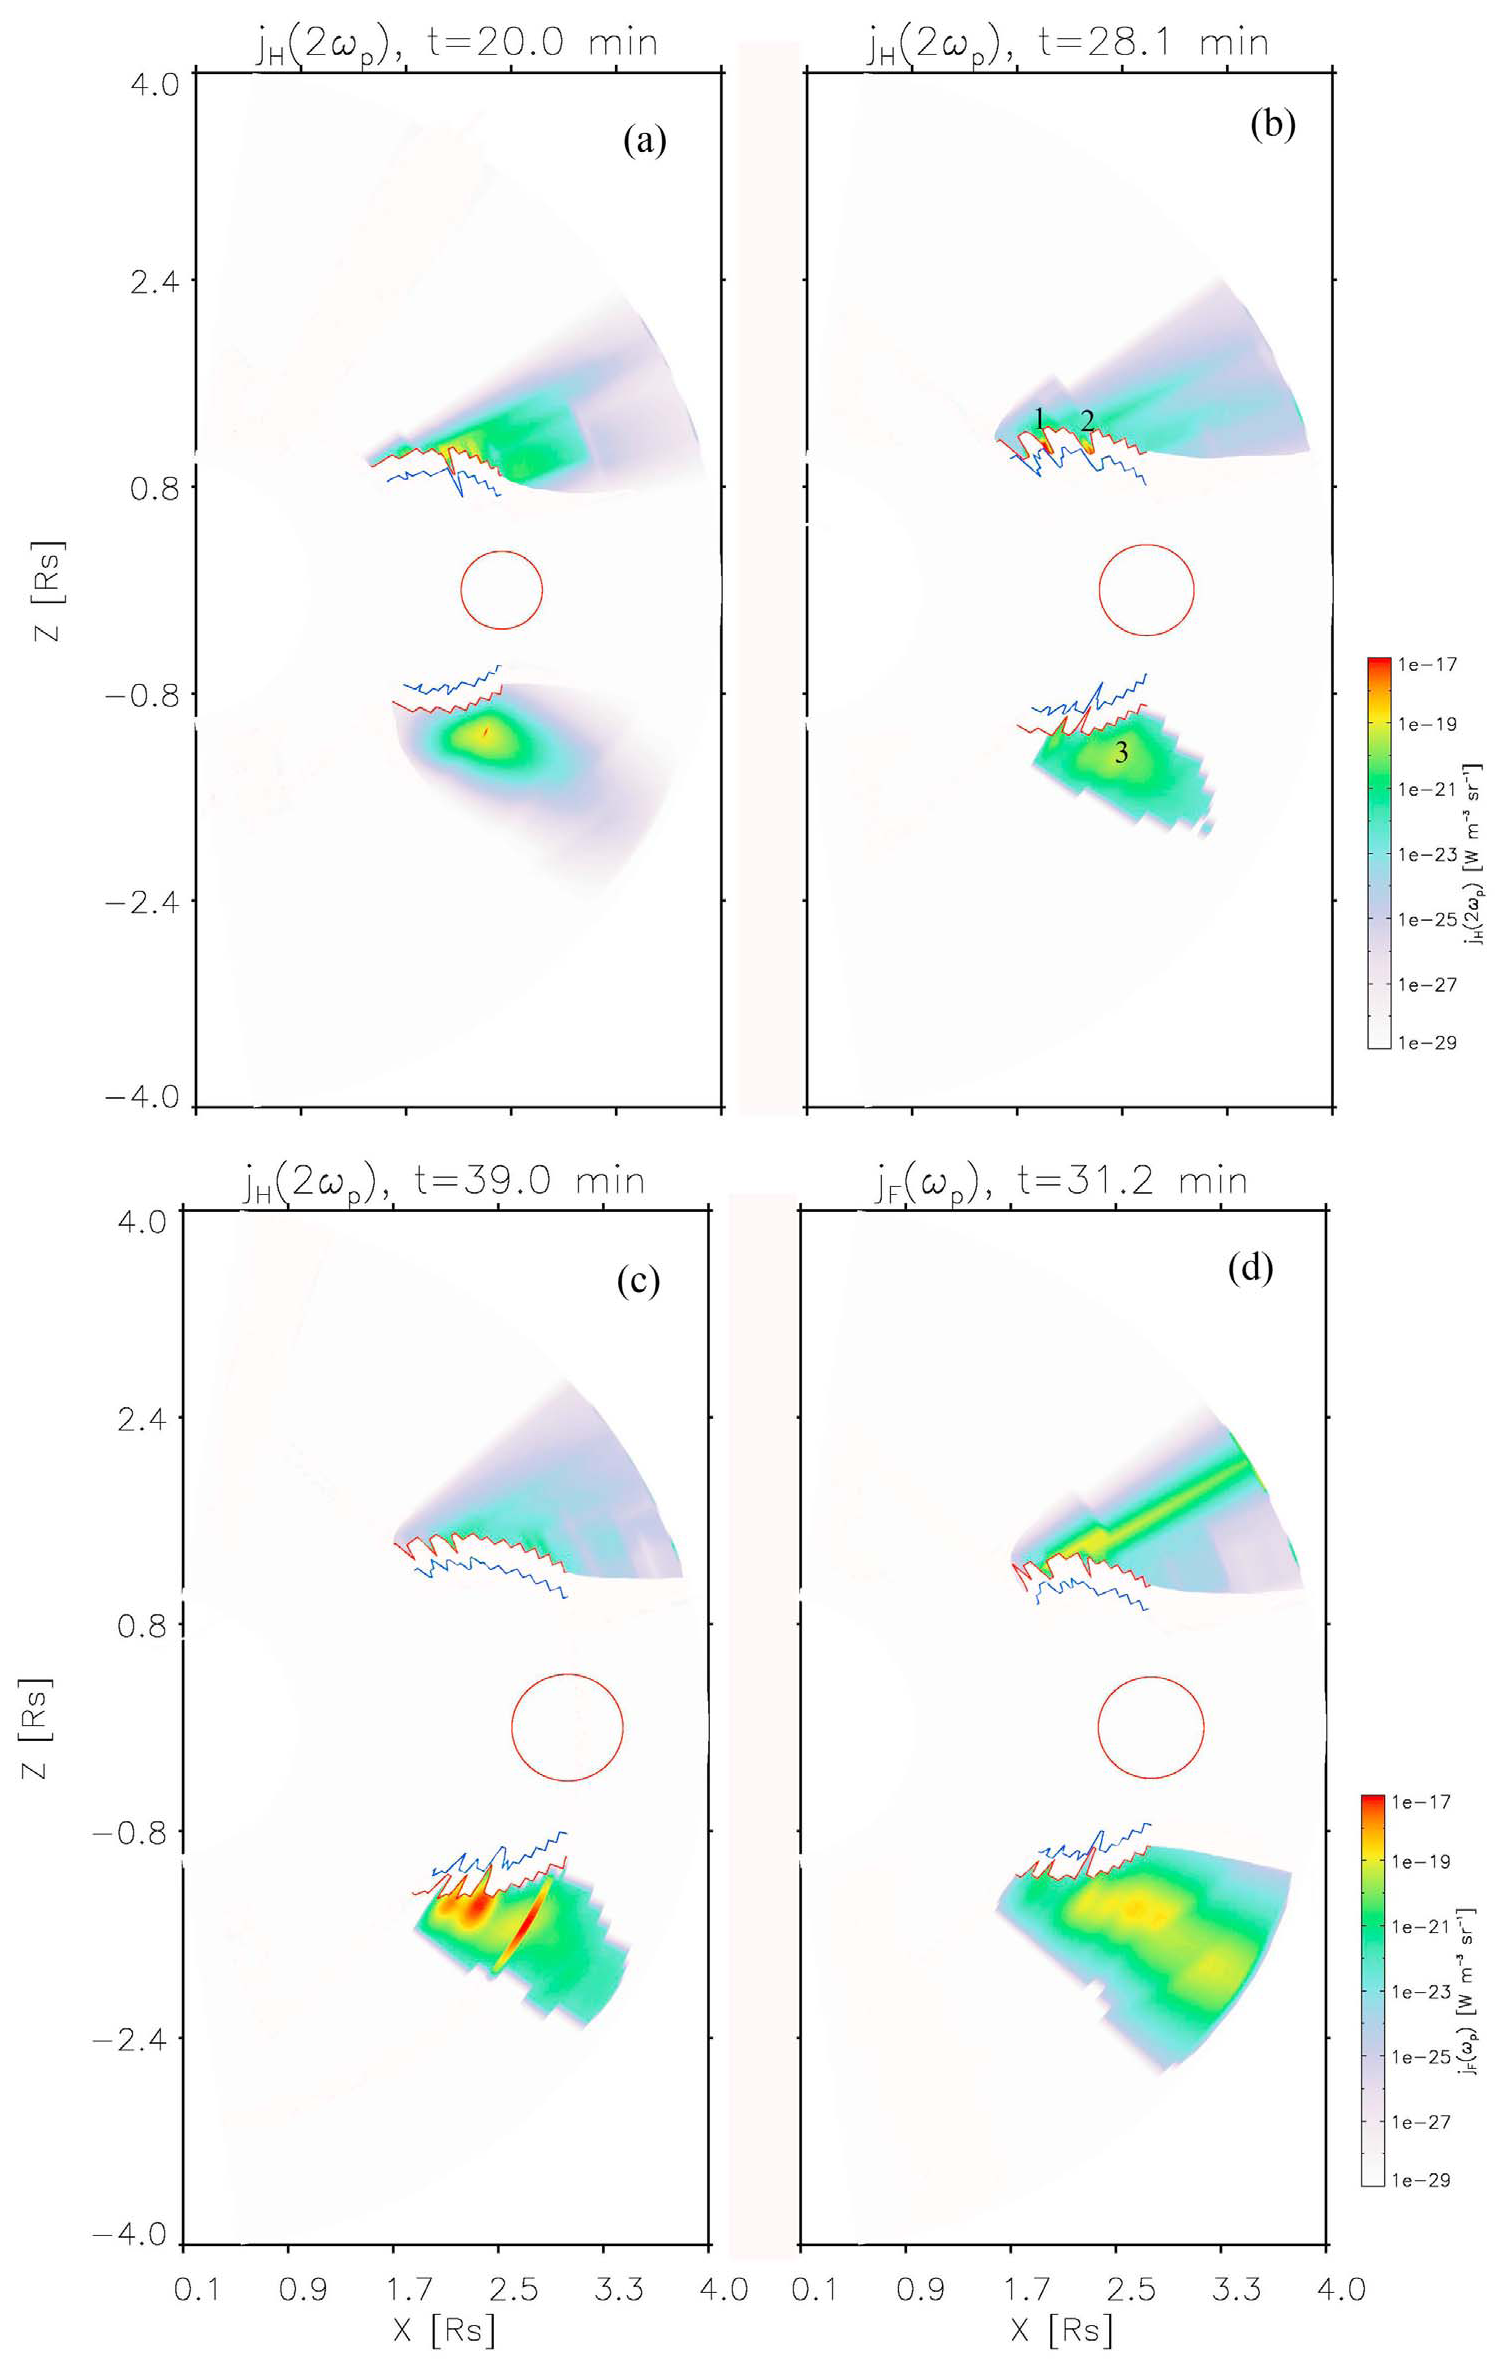
\includegraphics[scale=0.7]{schmidt_model}
%\caption[Model of radio burst driven by expanding CME flanks]{Complete model of radio burst driven by expanding CME flanks}
%\label{fig:schmidt_model}
%\end{center}
%\end{figure}
\begin{figure}[t!]
\begin{center}
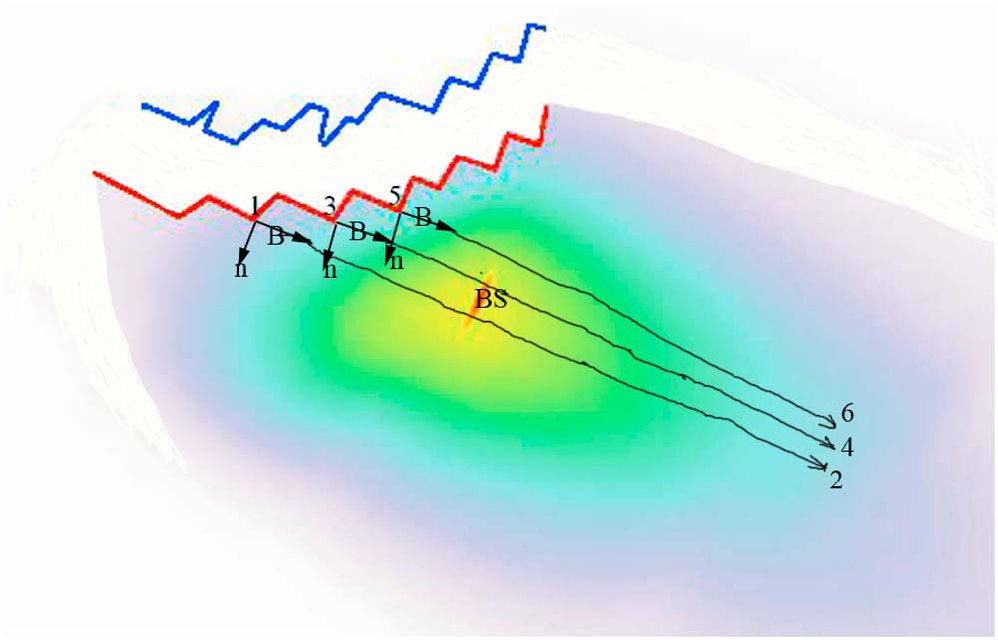
\includegraphics[scale=1.2]{herbone_model}
\caption[Model of radio burst driven by expanding CME flanks]{Model of the radio emission driven by electron beams on the flank of a CME. Each arrow marks the trajectory of the electron beams accelerated at the rippled shock surface. The red and blue lines outline the shock ramp. The green-red colours show radio emission intensity.}
\label{fig:herbone_model}
\end{center}
\end{figure}


\subsection{Frequency Drift of Radio Bursts}\label{sec:freq_drift}

In the previous section it was shown that when plasma emission is excited in the corona, the frequency of emission is close to the plasma oscillation frequency given by equation~\ref{eqn:plasma_frequency}
%As mentioned in section X, the frequency of emission allows a direct conversion from frequency to electron density of the environment in which the emission is generated. Since electron number density in the corona generally varies with height, it is then possible to calculate the height from which this frequency of emission came. To do this, a number of density models of the corona may be used, inclduing the Newkirk, the Saito, or the Baumbach-Allen. These provide a general description of the variation of electron density with height in the corona see Fig.~\ref{fig:density_models.}
As the exciter of the plasma emission moves to greater heights in the corona it will produce plasma emission at continually decreasing frequency due to the dropping density. For example a typical signature of a coronal shock wave in dynamic spectra is two narrow emission lanes (at $f_{plasma}$ and $2f_{plasma}$) drifting toward lower frequency as time passes. A type III radio burst is excited by a much faster source, hence its frequency drift is much faster in dynamic spectra. Generally different types of radio burst have different morphologies when viewed in dynamic spectra owing to their movement (or lack of movement) into regions of different density in the corona. A summary of the burst types is given in Figure~\ref{fig:radiobursts}
\begin{figure}[t!]
\begin{center}
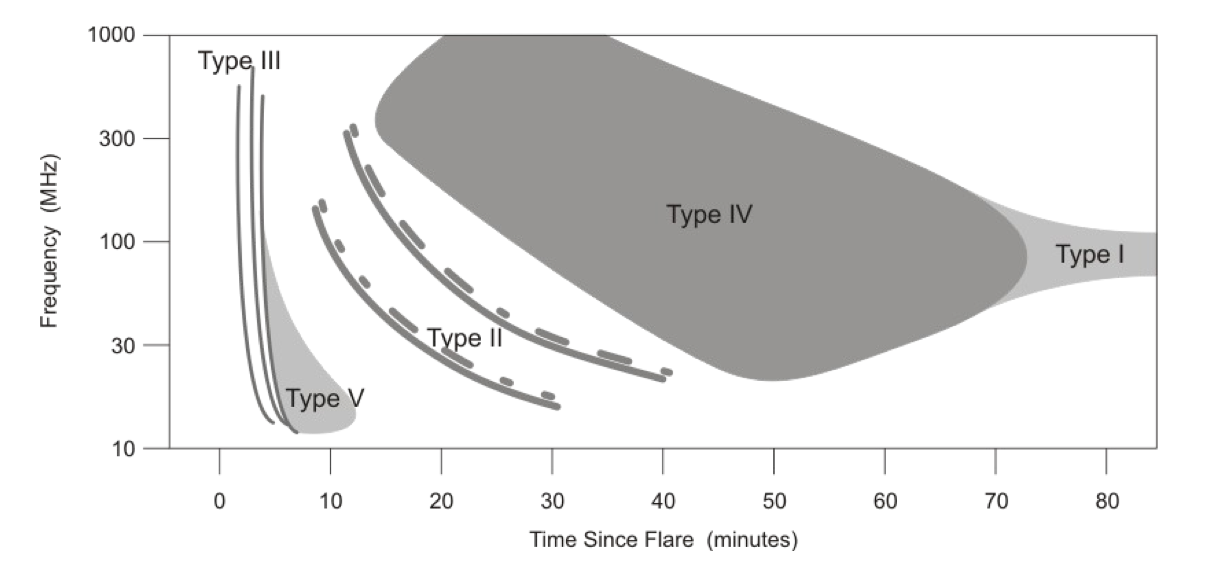
\includegraphics[scale=0.35, trim=2cm 0cm 0cm 2cm]{radiobursts.png}
\caption[Solar radio burst morphologies]{The characteristic shapes of various solar radio bursts seen in dynamic spectra. Type II radio burst are a signature of shock transit from high number density into low number density, as indicated by their drift from high to low frequency. The presence of two distinct bands is indicative of radio emission at the plasma frequency (fundamental) and its second harmonic. These two bands may also be further split themselves, a feature known as band-splitting.}
\label{fig:radiobursts}
\end{center}
\end{figure}

Generally, the frequency drift of the radio burst depends on the velocity of the exciter and the density variation in the corona. It is possible to estimate the speed of the exciter from a set of frequency time values $(f_i, t_i)$. Such as set of values are a direct diagnostic of the number density of the environment of emission versus time e.g., using $f \approx 9000\sqrt{n_e}$, frequency versus time gives number density versus time, $(f_i, t_i) \rightarrow (n_i,t_i)$.
Now, in general the number density of the corona is inversely proportional to height, varying according to some exponential decrease. A very simple model is the hydrostatic case $n(r) = n_0\mathrm{exp}(-r/H)$
\begin{figure}[t!]
%\begin{center}
\begin{minipage}[]{0.5\linewidth}
\centering
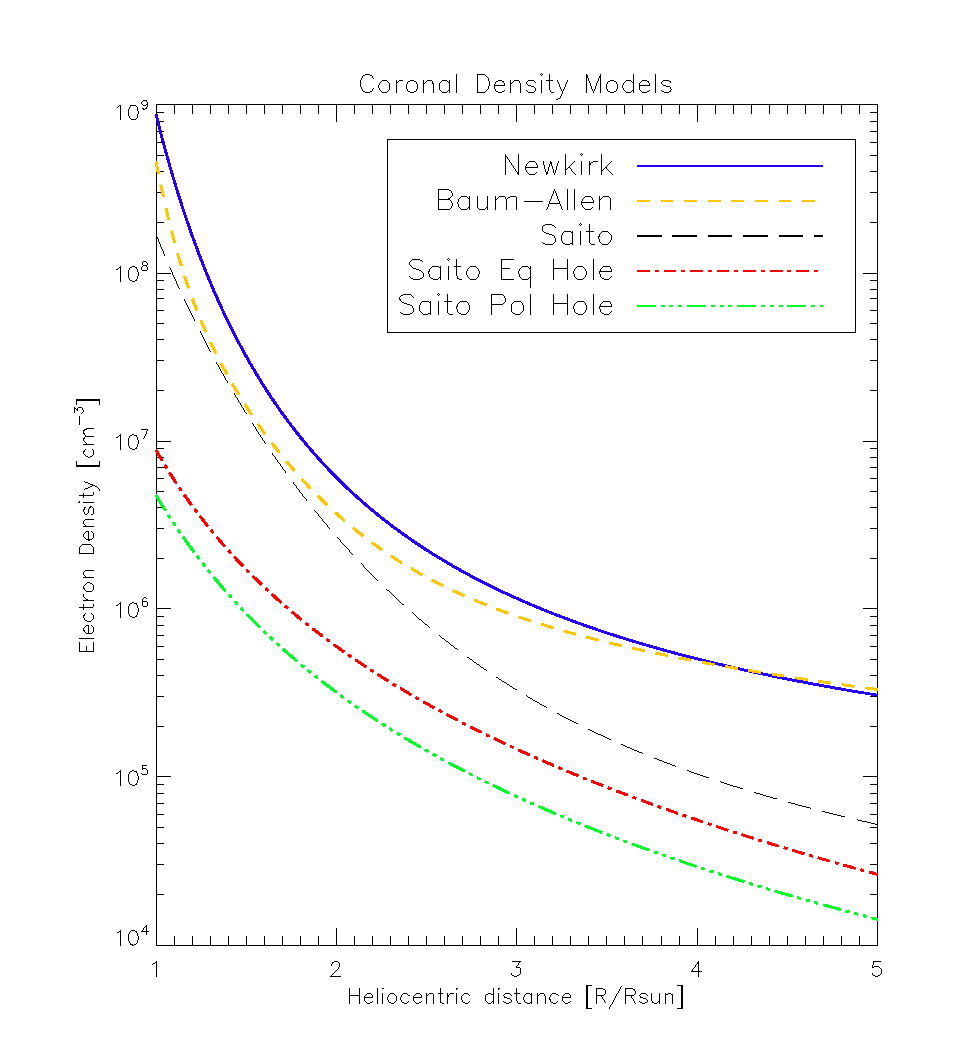
\includegraphics[trim= 2cm 0.0cm 0.0cm 2.0cm, scale=0.4]{density_models.pdf}
\end{minipage}
\hspace{0.1cm}
\begin{minipage}[]{0.3\linewidth}
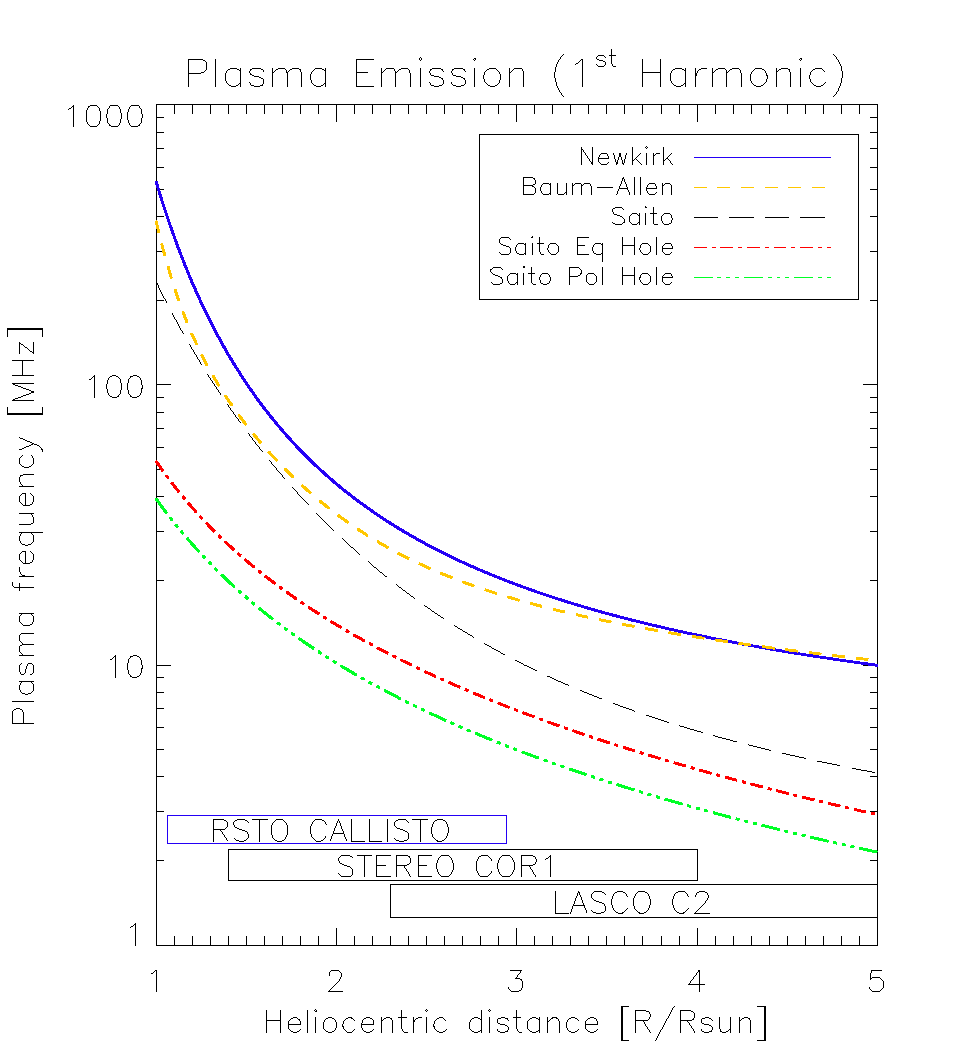
\includegraphics[scale=0.4, trim= 0cm 0.0cm 0.0cm 2.0cm]{1st_harmonic.pdf}
\end{minipage}
\caption[Various models for electron number density in the corona]{(Left)\,Electron number density as a function of height as defined by each of the models listed. The Newkirk, Baumbach Allen, and Saito models each describe an equatorial quiet corona electron density profile. The Saito Eq Hole and Pol Hol describe equatorial and polar hole profiles, respectively. These models are generally used to specify the height of a radio burst in the corona, and the choice of model is often arbitrary. (Right) The first harmonic of the plasma frequency as a function of height defined by the models.}% Added text here to elaborate differences between models
\label{fig:frequency_model}
\end{figure}
where $r$ is distance from sun center, and $H$ is the scale height given by $H = kT/mg$, where $k$ is Boltzman's constant, $T$ is the coronal temperature, $m$ is proton mass and $g$ is gravity. Generally using this $n(r)$, the set of values $(n_i,t_i)$ can be converted to as set of $(r_i,t_i)$
\begin{equation}
(f_i, t_i) \rightarrow (n_i,t_i) \rightarrow n(r) \rightarrow (r_i,t_i).
\end{equation}
Hence, by some appropriate choice of coronal density model $n(r)$, a set of frequency and time values may be converted to a set of height vs time values, from which the velocity may be derived.
%The derived shock velocity firstly assumes purely radial propagation of the shock, which is most likely not the case, and more importantly the method relies heavily on the choice of density model $n(r)$. 
Common practice is to use an $n(r)$ that is derived semi-empirically. For example, there exists a set of models that describe the density fall off with height of the equatorial quiet corona, coronal holes, and active regions \citet{allen1947, newkirk1961, saito1977}, shown in Figure~\ref{fig:frequency_model}. The choice of model affects both the resulting height of the radio emission and the derived speed. A much better diagnostic of radio bursts would be to use actual density measurements of the corona in places of these models, but this is generally not usual practice.

%In Figure 3.5 (left), there is a noticeable difference in both the range of densities and rate of decrease between each of these models. The choice of model to be used in the analysis of type II events is usually determined by the conditions that the shock is assumed to be propagating in. For example there could be propagation in an equatorial or polar coronal hole, through a quiet coronal background, or near an active region or streamer; the electron density is also known to vary with the cycle \citep{lamy2002}. 

%The choice of model affects both the resulting height of the radio emission and the derived speed. Also, even if the shock is known to be propagating in quiet coronal densities there is still a choice between a variety of models, such as the Saito, Newkirk and Baumbach-Allen models, each of which describe quiet equatorial corona. There is a noticeable difference between these models and the choice of one or the other, which is often arbitrary, will effect the resulting shock properties. Ultimately, the analysis of radio bursts are very heavily dependent on the coronal density model that is used, and there is no reason to favor one model over another.













%!TEX root = ../thesis.tex
%Adding the above line, with the name of your base .tex file (in this case "thesis.tex") will allow you to compile the whole thesis even when working inside one of the chapter tex files


\chapter{Observation and Instrumentation} 
\label{chap:2}

\section{Thompson Scattering Theory}\label{sec:3}

\subsection{The van de Hulst Coefficients}\label{sec:30}

\subsection{Thomson Scattering in the Corona}\label{sec:31}

\subsection{White-light observations of CMEs}


\section{Conornagraphs}\label{sec:1}

\subsection{SOHO LASCO}\label{sec:10}

\subsection{STEREO CORs}\label{sec:11}



\section{Radio Spectrometers and Radioheliographs}\label{sec:2}

\subsection{Callisto}\label{sec:20}

\subsection{Nancay Decametric Array}\label{sec:21}

\subsection{Nancay Radioheliograph}\label{sec:22}



\section{EUV imaging}\label{sec:3}

\subsection{SDO AIA}\label{sec:30}




%!TEX root = ../thesis.tex
%Adding the above line, with the name of your base .tex file (in this case "thesis.tex") will allow you to compile the whole thesis even when working inside one of the chapter tex files

\singlespacing
\chapter{Coronal Mass Ejection Masses, Energetics, and Forces} 
\label{chap:4}
\vspace{-6mm}
\doublespacing
In the past, measurement of CME dynamics have been hindered by highly uncertain estimates of the total mass of the ejection. The primary source of uncertainty is the unknown position and geometry of the CME, leading to an erroneous treatment of the Thomson scattering equations which are used to estimate the mass. Geometrical uncertainty on the CMEs position and size has primarily been due to observations of the eruption from a single vantage point. However, with the launch of the {\it Solar Terrestrial Relations Observatory (STEREO)} mission, the two viewpoints can be exploited to derive the CMEs position and size, ultimately resulting in mass uncertainty that is both reliably quantified and much reduced. This then leads to better estimates of the energies and forces. This chapter will first outline the Thomson scattering theory used to compute CME mass, followed by a discussion of the mass uncertainties. This work includes the smallest uncertainties in the literature on CME mass, and the first estimate CME force magnitude from observations. This chapter is based on work published in Carley, McAteer, \& Gallagher, {\it The Astrophysical Journal}, 2012.

\section{Introduction}\label{sec:1}

Despite many years of study, the origin of the forces that drive coronal mass ejections (CMEs) in the solar corona and interplanetary space are not well understood. From an observational viewpoint a complete understanding of CME kinematics, dynamics and forces requires not only a study of CME speed, acceleration and expansion but also an accurate knowledge of CME mass.  The measurements of CME mass combined with acceleration measurements can be used to quantify the magnitude of the force that drives a CME. Knowledge of this force magnitude can lead to an identification of the possible origin of the CME driver. 

There are numerous theoretical models that attempt to explain the triggering of CME eruption and its consequent propagation. Each describe the destabilization and propagation of a complex magnetic structure, such as a flux rope, via mechanisms that include the catastrophe model \citep{forbes1991,forbes1995,lin2000}, magnetic breakout model \citep{antio99,lynch2008}, or a toroidal instability model \citep{chen1996,kleim2006}, each described in Chapter 2. The loss of equilibrium induced by such mechanisms results in CME propagation into interplanetary space. The predictions of these models have been investigated in observational studies whereby the CME kinematics are used to constrain what forces might be at play and hence which model best describes CME propagation. Such studies show that early phase propagation can be reasonably described by the existing models (or a combination of them) involving some form of magnetic CME driver \citep{manoh2003, chen2006, schrijver2008c, lin2010}, and that aerodynamic drag of the solar wind may have a significant role at later stages of CME propagation \citep{howard2007, malo10, byrne2010}. Comparisons between modeling and observational estimates of the forces that drive CMEs requires an accurate determination of CME kinematics properties as well as CME mass.

To date, the most prevalent method of determining CME mass has been through the use of white light coronagraph imagers, such as the Large Angle Spectroscopic Coronagraph  \citep[LASCO;][]{bru95} on board the \emph{Solar and Heliospheric Observatory} \citep[\emph{SOHO};][]{dom95}  and the twin Sun Earth Connection Coronal and Heliospheric Investigation (SECCHI) COR1 and COR2 coronagraphs \citep{how08} on board the \emph{Solar Terrestrial Relations Observatory}  \citep[\emph{STEREO};][]{kai08}. The white-light emission imaged by such coronagraphs occurs via Thomson scattering of photospheric light by coronal electrons \citep{min30, vdeh50, bil66}, the so called K-corona.  From classical Thomson scattering theory, the intensity of the light detected by an observer depends on the particle density of the scattering plasma. Hence, any density enhancement, such as a CME, over the background coronal density appears as enhanced emission in white light. The enhanced emission allows for a calculation of the total electron content and hence mass. 

Some of the first measurements of CME mass using scattering theory were carried out by \citet{munro1979} and \citet{poland1981} using space-based white light coronagraphs on board \emph{SkyLab} and U.S. military satellite\,\emph{P78-1}.  Both the early studies  and later statistical investigations determined that the majority of CMEs have masses in the range of 10$^{13}$--10$^{16}$\,g, \citep{vourlidas02, vour2010}. However, due to only a single viewpoint of observation, the longitudinal angle at which the CME propagates outwards was largely unknown in these studies 
and it is generally assumed that the CME propagates perpendicular to the observers line-of-sight (LOS). There is also the added assumption that all CME mass lies in the two-dimensional plane-of-sky (POS). Such assumptions can lead to a mass underestimation of up to 50\% or more \citep{vou00}. More recent studies have employed the two viewpoint capabilities of the \emph{STEREO} mission to determine the mass of numerous 
CMEs with much less uncertainty \citep{cola09}. 
	
This Chapter presents an analysis of mass development of the 2008 December 12 CME using the \emph{STEREO} COR1 and COR2 coronagraphs. We use a well constrained angle of propagation to determine the mass and position of the CME. Combining the mass measurements with values for CME velocity and acceleration, the kinetic energy and the magnitude of the force influencing propagation is determined for each point in time. The first section described the observations of the event from first appearance of the front in COR1 A and B to the time when the front exits the COR2 A and B fields of view. 
The data analysis section describes the methods by which the masses are calculated with \emph{a priori} knowledge of the propagation angle, as well as a discussion of the primary sources of uncertainty. Followed by this are the results, including masses, energies and forces on the CME. Finally, a discussion is given of the possible forces attributable to the observed accelerations and whether they are magnetic or aerodynamic in origin. 

\section{Observations}

The COR1 images used in this analysis span from 2008 December 12 04:05\,UT to 15:45\,UT, with a cadence of 10\,minutes. The three polarization states of COR1 were combined to make total brightness images in units of mean solar brightness (MSB). Base difference images were produced using the 04:05\,UT image (in both COR1\,A\,and\,B) as a background to be subtracted from all subsequent images. A sample of such images for both COR1\,A and B can be found in Figure~\ref{fig:STEREO_COR1A&B}. The COR2 images analyzed range from from 07:22\,UT to 17:52\,UT, with a cadence of 30\,minutes. As with the COR1 images, total brightness images were created for COR2, and a set of base difference images were then produced using the 07:22\,UT image as a suitable background. A selected set of images from COR2 can be found in Figure~\ref{fig:STEREO_COR2A&B}. Note that the pixel values in Figures~\ref{fig:STEREO_COR1A&B} and~\ref{fig:STEREO_COR2A&B}  have been converted to grams; the method by which this is done is described in the next section.
	
At 04:35\,UT the leading edge of a CME appeared in COR1\,A and B coronagraphs at a height of $\sim$1.4\,$R_{\odot}$, off the east and west limb respectively. In COR1\,B the CME first appears as a set of rising loop-like structures followed by a prominence, part of which appears to fall back to the surface at 08:00\,UT while the remainder was ejected and follows the rising loop-like structures which eventually become the CME front. The rising prominence was not apparent at any stage of the propagation in COR1\,A and the advancing front remains the only distinguishable facet 
of the CME from this line-of-sight (LOS).
\begin{sidewaysfigure}
    \centering
	\includegraphics[scale=0.6]{cor1ab_color.pdf}
	\caption [2008-December-12 CME observed by COR1] {Selection of base difference images of the CME in COR1\,A  
	(top row) and COR1\,B (bottom row). The CME is quite faint in the A images and appears not to have as much structure
	as in B. As indicated by the color bar on the right, this image has units of grams. The method by which pixel units of 		grams are derived is described below.}
\label{fig:STEREO_COR1A&B}
\end{sidewaysfigure}

\begin{sidewaysfigure}
    \centering
    \includegraphics[scale=0.6]{cor2ab_color.pdf}
	\caption [2008-December-12 CMe observed by COR2]{Selection of base difference images of the CME in COR2\,A (top 	row) and COR2\,B (bottom row), with pixel values of grams. The CME is 
	clearly distinguishable in both fields of view. Only the B field view shows clearly the three part structure of core, cavity 	and front. As with the COR1 images these images also have units of grams; the method by which grams are calculated 	is described below.}
\label{fig:STEREO_COR2A&B}
\end{sidewaysfigure}    

A noteworthy caveat of using base difference imaging is the assumption that the background corona in the pre-event image has the same brightness in all subsequent images. This may not always be true and any excess brightness in the pre-event image will produce negative pixel values in the base difference. This is apparent in the COR1 images as the CME interacts with a streamer, displacing it as the leading CME front expands laterally as well as moves outward. The streamer is visible as a dark feature that grows with time at the southward flank of the CME in the COR1\,B images, Figure~\ref{fig:STEREO_COR1A&B}. The black areas are indicative of negative pixel values. The COR1\,A images also suffer from negative pixels, especially at later times, see Figure~\ref{fig:STEREO_COR1A&B} top row, 09:15\,UT image. 
The front of the CME starts to exit both the A and B field of view at $\sim$08:35\,UT.

The CME first appears in the COR2 field of view at $\sim$07:52\,UT with the CME apex at a height of $\sim$3\,$R_{\odot}$ in both A and B images. In the B coronagraph, by 10:52\,UT the three part structure of core, cavity, and bright front is clearly visible and the overall structure grows in size as the CME propagates to larger heights. The core becomes more tenuous and the mass distribution becomes homogenous after 15:52\,UT when the front starts to exit the field of view. The distinction between core and front is not as clear in COR2\,A and the mass distribution appears more homogenous throughout the propagation. As with the COR1 images, COR2\,A is also affected by excess brightness in the pre-event image, as is apparent by a growing dark feature in its southern half. As the pre-event image for COR2\,B is the cleanest of the pre-event images (it contains the least contamination by streamers), the COR2\,B data are considered the best candidate for accurate CME mass measurements. 



\section{Data Analysis}\label{sec:10}

A conversion from pixel units of mean solar brightness to grams requires a knowledge of how electrons scatter photospheric light in the corona. A brief overview of the theory is given here, along with a discussion of the uncertainties due to some unknowns about the CME position and shape.

\subsection{Thomson Scattering in the Corona}\label{sec:10}
\doublespacing
Thomson scattering involves an incident electromagnetic wave exciting an oscillation of an electron such that the electron radiates like a small dipole. In this way some of the incident electromagnetic energy is `scattered' in a variety of directions, given by the radiation pattern of the oscillating electron. Any incident radiation falling on the area
\begin{equation}
\sigma_T = \frac{8\pi}{3}\bigg(  \frac{e^2}{4\pi\epsilon_0 m_e c^2}   \bigg)^2 = \frac{8\pi}{3}r_e^2 = 6.65\times10^{-29}\,\mathrm{m}^2
\end{equation}
will be scattered by the electron into a dipole radiation pattern. $r_e$ is the classical electron radius and the cross section used in the following analysis will be $\sigma_e = r_e^2$. The area is the Thomson scattering cross-section and is independent of wavelength of the incident wave; all wavelengths are scattered equally. 

\begin{figure}[!t]
\begin{center}
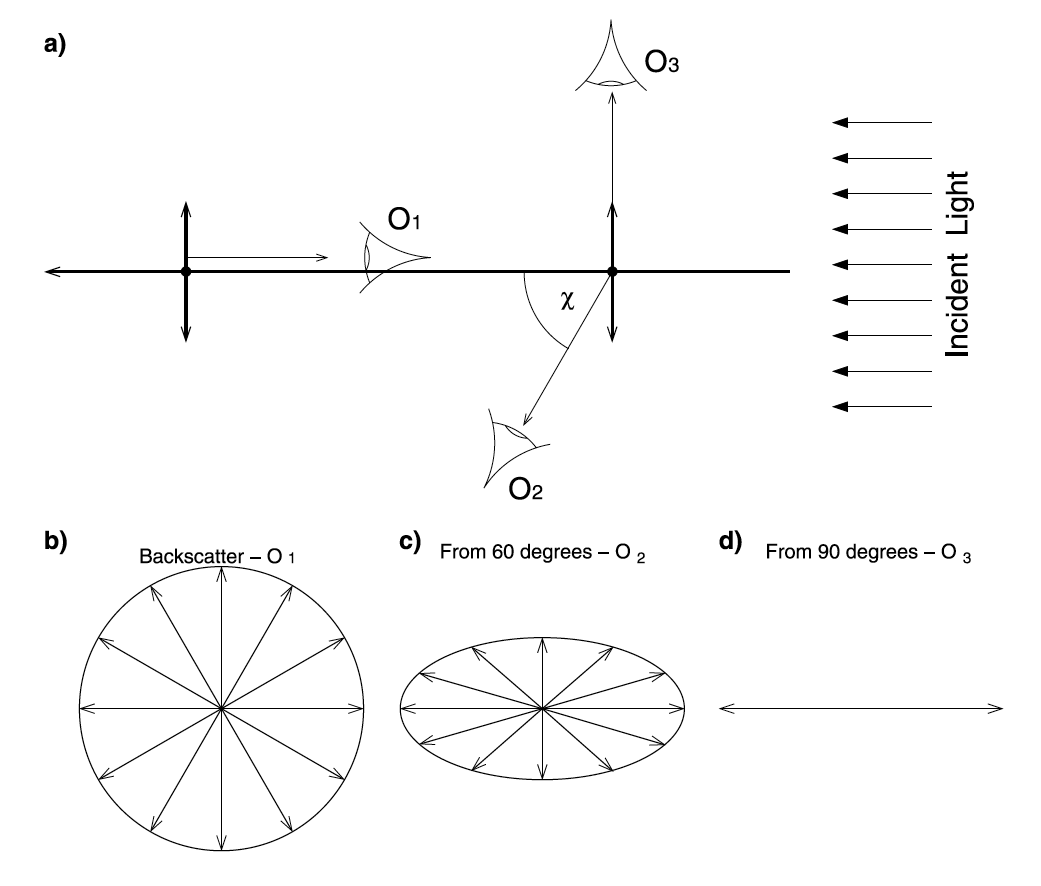
\includegraphics[scale=0.35, trim=1cm 0cm 0cm 0cm]{t_scatter}
\caption[Thomson scattering schematic.]{Thomson scattering schematic \citep{howtap2009}.}
\label{fig:tscatter}
\end{center}
\end{figure}
Solar photospheric radiation is completely unpolarized, hence the radiation incident on a coronal electron with set it into an oscillation with an amplitude that is equal in all directions. In Figure ~\ref{fig:tscatter}, their are two components to the incoming light, setting the electron into oscillation parallel to the page and perpendicular to it. No matter what the viewing angle, $\chi$, the perpendicular oscillation will always be observed to have the same amplitude. However, the parallel component will be fore-shortened, depending on $\chi$. In this way, the radiation may appear unpolarized, partially polarized, or completely linearly polarized.

\citet{schuster1879} and \citet{minnaert1930} were the first to formalise the Thomson scattering theory for an electron in the solar atmosphere. The electron is set into oscillation by an unpolarized  incident intensity $I_0$.
The two components of radiation observed are the tangential component, $I_T$ in the plane perpendicular to the page, and radial component, $I_R$ in the plane of the page Figure~\ref{fig:omega}. 
These two components are given by the expressions \citep{howtap2009}
\begin{eqnarray}
I_T &=& I_0\frac{\pi \sigma_e}{2z^2}[(1-u)C +uD] \\
I_P &=& I_0\frac{\pi \sigma_e}{2z^2}\mathrm{sin}^2\chi[(1-u)A +uB] \\
I_R &=& I_T-I_P
\end{eqnarray}
where $I_0$ is incident intensity, $\sigma_e$ is the electron scattering cross section, $z$ is the distance from scatterer to observer, $u$ is a limb darkening coefficient. $I_R$ is given via a polarization intensity $I_P$ for ease of derivation. These equations describe theoretically the concepts outlined in Figure~\ref{fig:tscatter} e.g, both $I_T$ and $I_R$ are fully observed at $\chi=0^{\circ}$ and $\chi=180^{\circ}$, while only $I_T$ is observed at $\chi=90^{\circ}$. 
\begin{figure}[!t]
\begin{center}
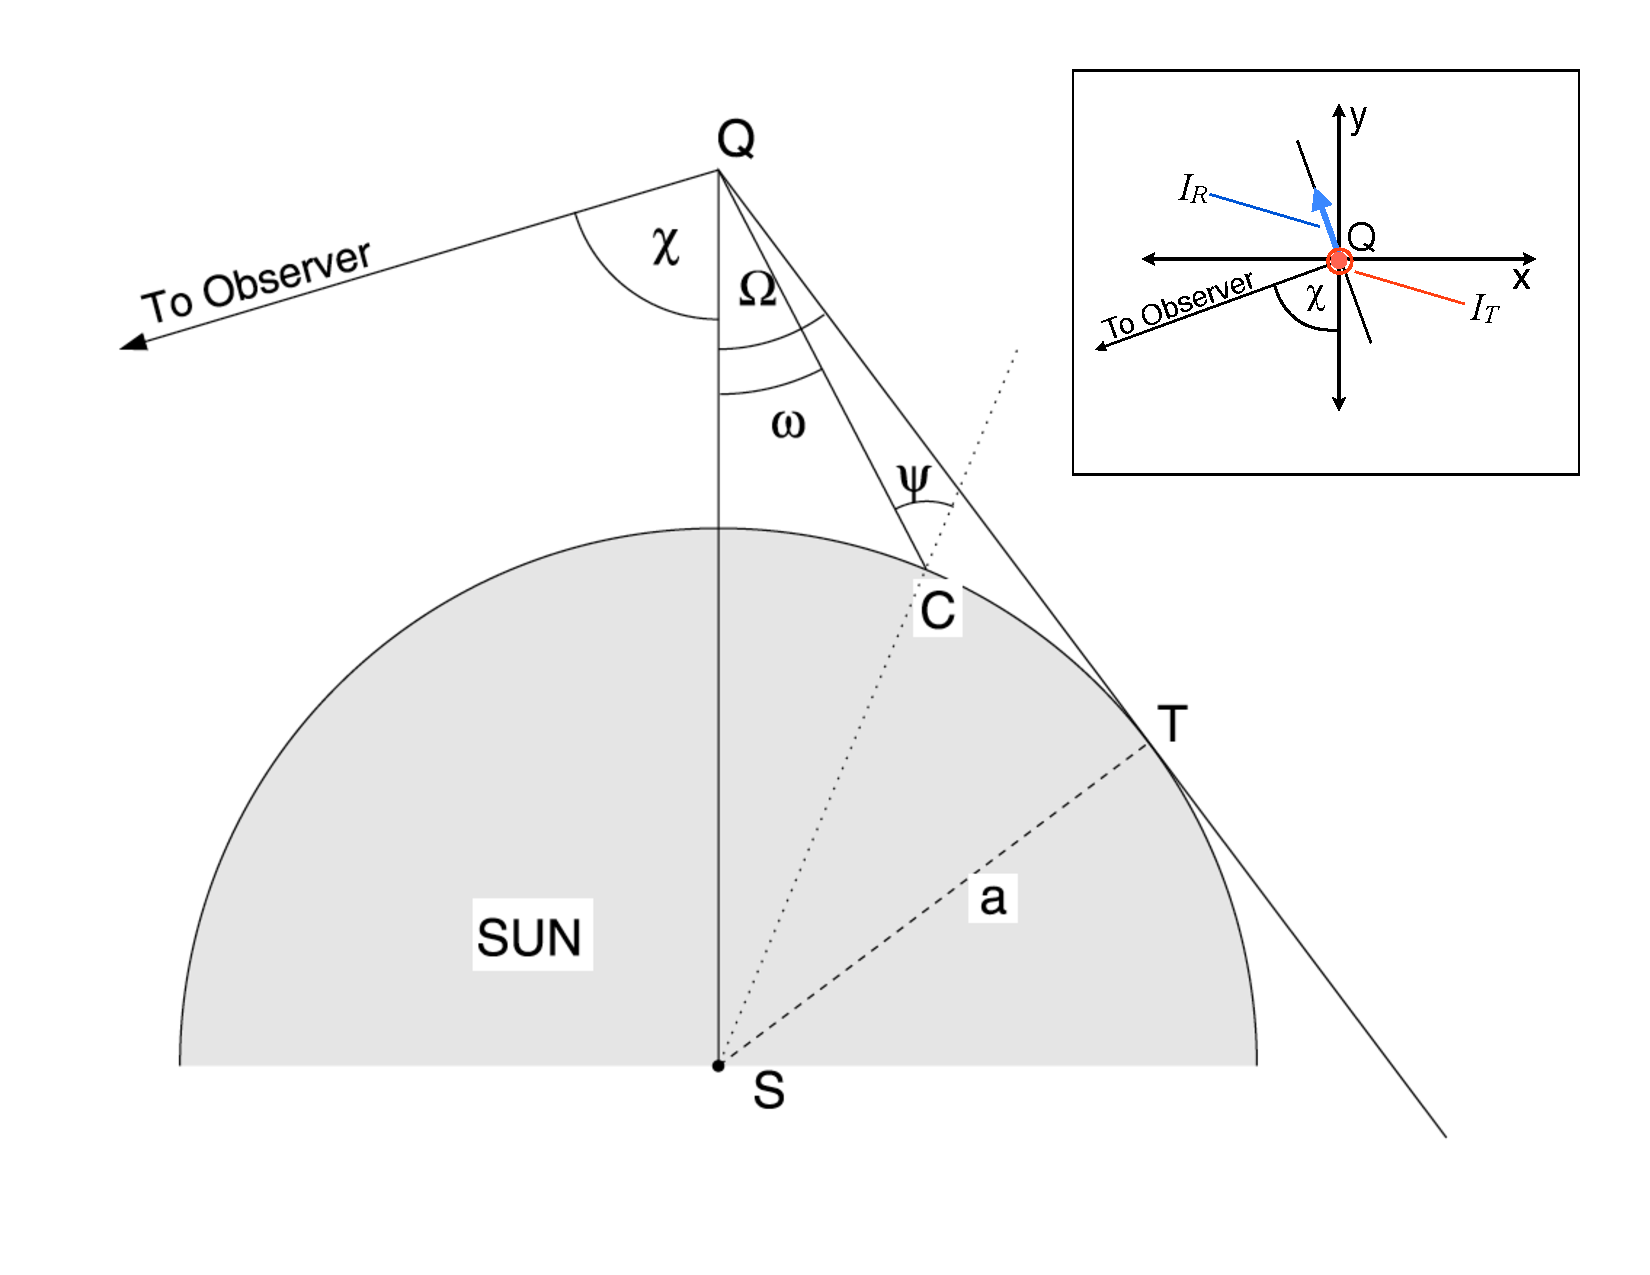
\includegraphics[scale=0.5, trim=0cm 2cm 0cm 0cm]{omega_new.pdf}
\caption[Thomson scattering geometry in the solar corona]{Thomson scattering geometry in the solar corona. The orientation of $I_R$ and $I_T$ is shown in the inset. $I_R$ is the projection of electron oscillation in the x direction onto a plane perpendicular to the line from Q to observer. $I_R$ is zero when $\chi=90$. $I_T$ is due to electron oscillation out of the plane of the page (z-direction), and is completely unaffected by viewing angle. Figure adapted from Figure 3 of \citep{howtap2009}.}
\label{fig:omega}
\end{center}
\end{figure}
The main complication for Thomson scattering by a coronal electron is that the Sun is not a point source. The effects of the finite size of the Sun are incorporated into $A$, $B$, $C$, and $D$ in equations (4.2)--(4.4). These are trigonometric expressions known as the van de Hulst coefficients \citet{vdeh50}, and completely characterise the reception of light by the electron from across the entire solar disk, using only the angle $\Omega$, the angle subtended by the solar disk from point Q shown in Figure~\ref{fig:omega} \citep{minnaert1930, billings1966, billings1966} 
\begin{eqnarray}
A &=& \cos \Omega \sin^2 \Omega \\
%
B &=& -\frac{1}{8}\bigg[1 - 3\sin^2\Omega -\frac{\cos^2\Omega}{\sin\Omega}(1+3\sin^2\Omega)\textrm{ln}\bigg(\frac{1+\sin\Omega}{\cos\Omega}\bigg)\bigg] \\
%
C &=& \frac{4}{3} - \cos\Omega - \frac{\cos^3\Omega}{3} \\
%
D &=& \frac{1}{8}\bigg[5 + \sin^2\Omega -\frac{\cos^2\Omega}{\sin\Omega}(5-\sin^2\Omega)\textrm{ln}\bigg(\frac{1+\sin\Omega}{\cos\Omega}\bigg)\bigg] 
\end{eqnarray}
These coefficients and equations (4.2)--(4.4) form a complete description of the light scattered by an electron at any position in the solar atmosphere (any $\Omega$), with the observer at viewing angle $\chi$. The intensities given by these equations are for a single electron. If there is a number of electrons $N_e$, then the intensity would simply be $IN_e$; the intensity of scattered light from a point Q depends linearly on the total number of scattering electrons at that point. Hence if we know the intensity of scattered light we may directly infer the total number electrons contributing to this intensity. This allows a calculation of the total electron content of a CME, resulting in a mass calculation. However, the mass calculation os very sensitive to $\chi$, the viewing angle, and some important aspects of CME observation arise from this.

%As mentioned the above equations have a sensitive dependence of intensity and polarization on scattering angle $\chi$. The total intensity of scattered light is
%\begin{equation}
%I_{tot} =  2I_T - I_p \propto I_0\frac{\pi \sigma_e}{z^2}\bigg(1 - \frac{\mathrm{sin}^2\chi}{2}\bigg)
%\end{equation}
%So at $\chi=90$, $I_p$ is maximum, $I_R$ is minimum, $I_{tot}$ is minimum, and scattering efficiency is minimum. The dependency of each intensity component is shown in Figure~\ref{fig:Ivchi}. The tangential component $I_T$ remains constant at all viewing angles, whereas $I_R$ is maximum at $0^{\circ}$ or $180^{\circ}$ and minimum at $90^{\circ}$. Polarization is maximum at $90^{\circ}$. 
%\begin{figure}[!t]
%\begin{center}
%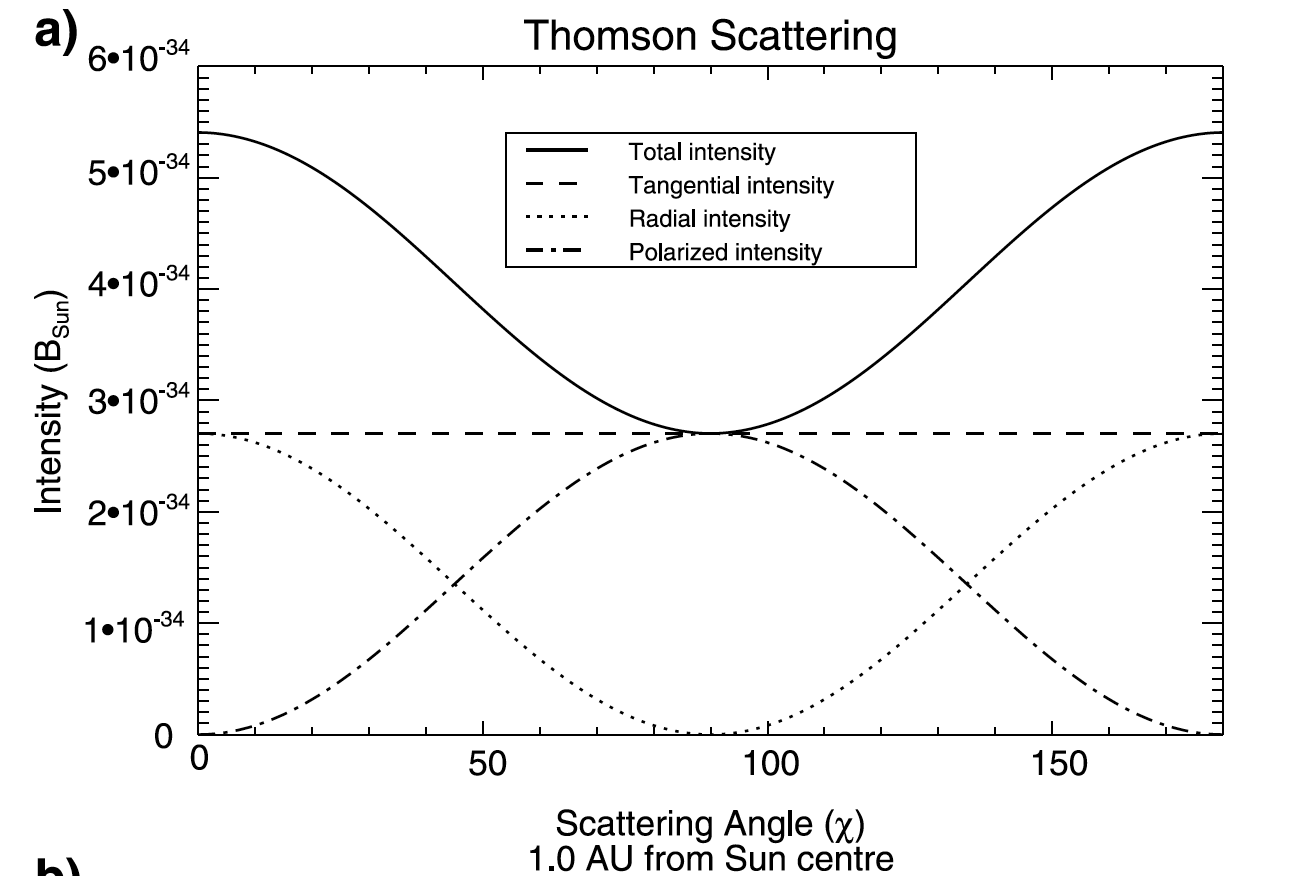
\includegraphics[scale=0.3]{IT_IR}
%\caption[Thomson scattered intensity as a function of viewing angle]{Thomson scattered intensity as a function of viewing angle.}
%\label{fig:Ivchi}
%\end{center}
%\end{figure}

Along any line of sight through the corona, the point at which $\chi = 90^{\circ}$ will be the point of minimum distance from the Sun. Three effects must be considered at this point; (i) scattering efficiency is a minimum, (ii) the incident intensity ($I_0$) received from the Sun is a maximum, and (iii) the electron density is a maximum. The latter two effects, (ii)--(iii), are a bigger contributor to the scattered light than the former (i). As a result scattered light is maximized at the point of $\chi = 90^{\circ}$ along the line of sight, despite the efficiency of scattering being a minimum at this point. Close to the Sun, the plane making an angle of $\chi = 90^{\circ}$ with the line of sight is known as the plane-of-sky (POS), and is the plane of maximum scattered intensity. Any CME erupting close to the POS will be well observed. However, eruption of a CME at a large angle away from the POS will result in less scattered light from the CME electrons, making the CME appear quite faint. If the angle from the POS is unknown, there is no way of telling the amount by which the intensity is reduced. 
%Observing a smaller intensity will result in the observer calculating a smaller number of electrons contributing to the scattered light. If no correction is made for the diminished intensity, the number of electrons and hence the total CME mass will be underestimated. The correction can only be made when the angle from the POS is known. As if often the case, the angle is unknown and we must assume the CME lies on the plane of sky. If this assumption is false, there will a proportion of the CME that we will go unaccounted for, 
This can lead to an underestimation of its mass content by up to a factor of 2 \citep{vou00}. As described in the next section, unknown viewing angles are the largest contributor to CME mass uncertainty.





\subsection{Mass Measurements and Uncertainties}
\begin{figure}[t!]
\begin{center}
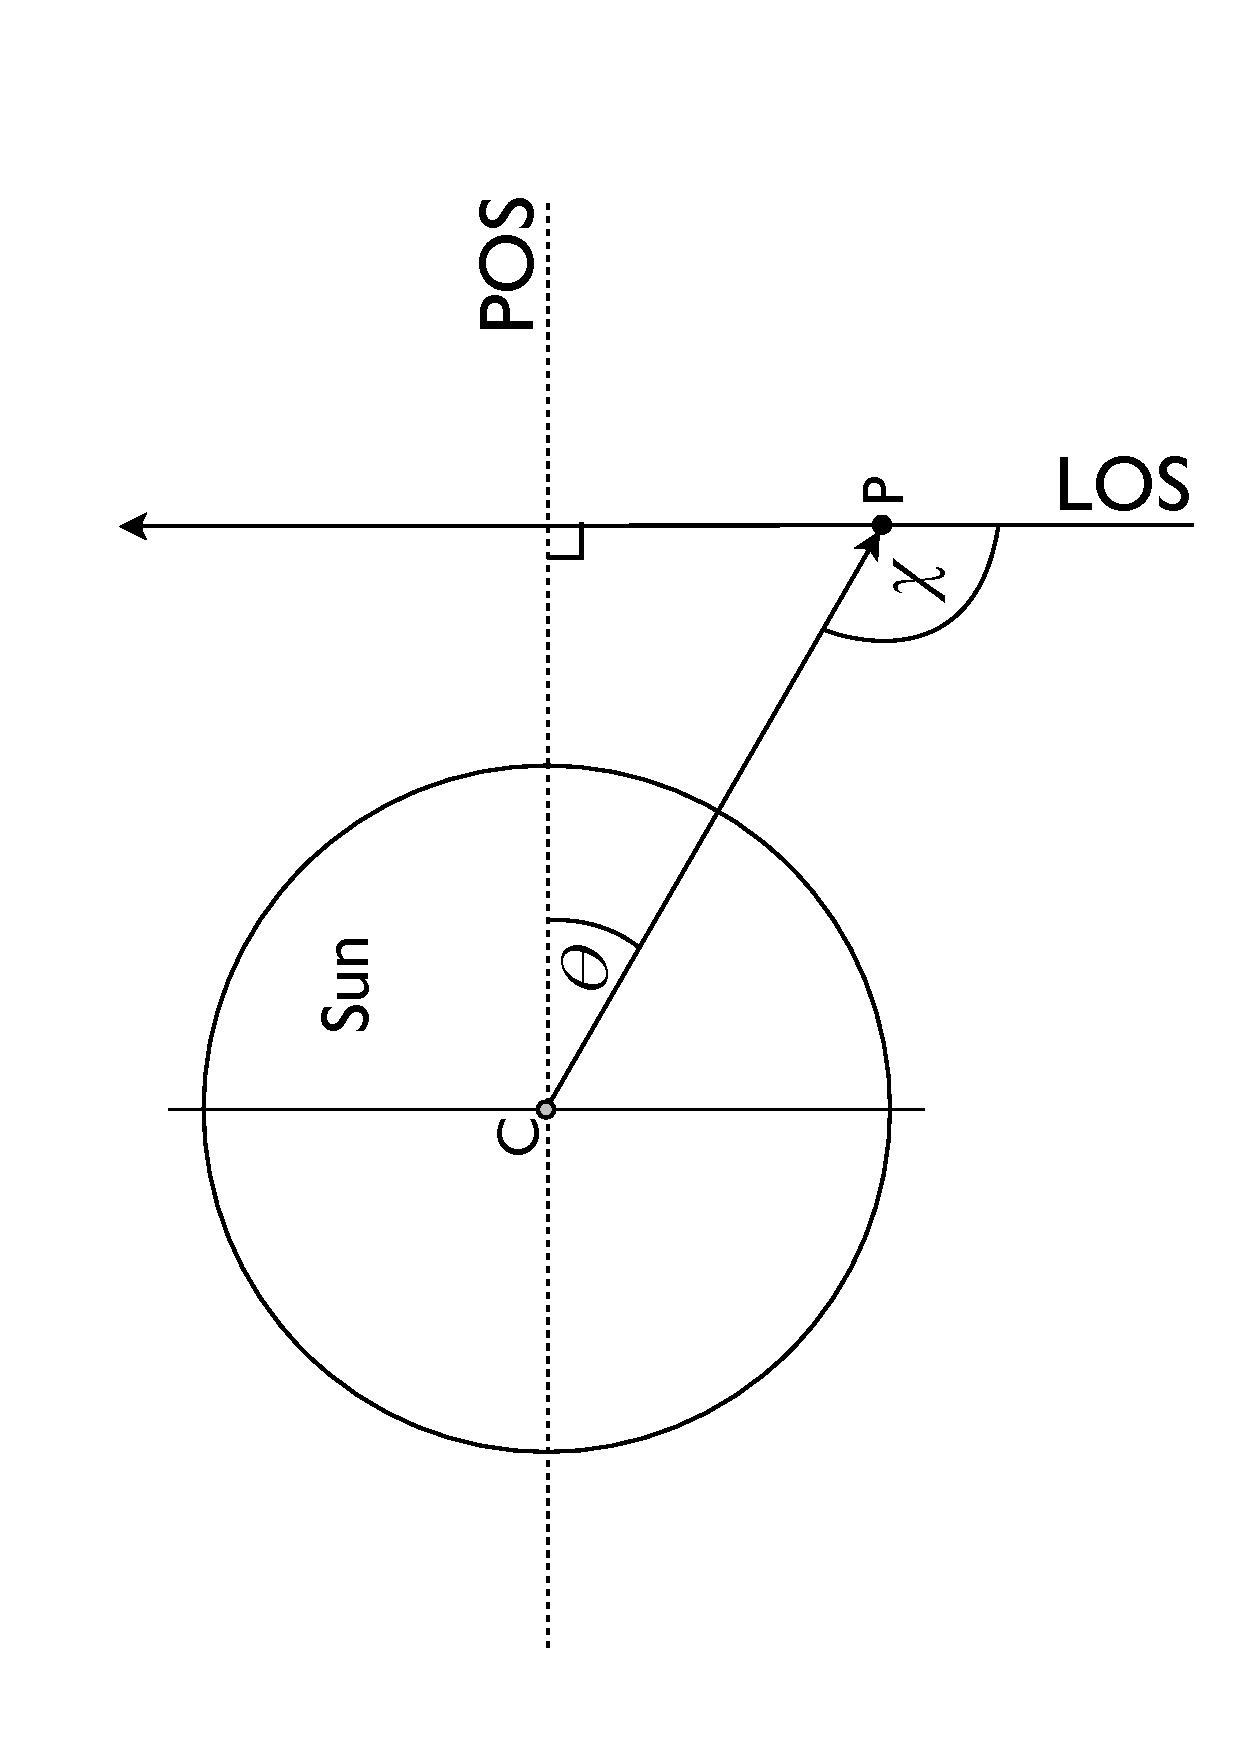
\includegraphics[trim = 0cm 0cm 0cm 0cm, scale=0.4, angle=270]{images/LOS_POS_2.pdf}
\caption[Line-of-sight and plane-of-sky orientations]{Schematic showing the relative orientation of the line-of-sight (LOS), and the plane-of-sky (POS). Electron position is at point P and C is 
Sun center. The vector CP may also represent CME propagation direction. Scattering efficiency is heavily dependent on the angle $\theta$ 
(or $\chi$) and is least efficient 
when $\theta = 0^{\circ}$ ($\chi=90^{\circ})$.}
\label{fig:LOS_POS_2}
\end{center}
\end{figure}
%
%
%
Calculating the total mass of a CME requires an estimate of the total amount of electrons contributing to the light scattered by the CME. Then assuming that the corona is 90\% hydrogen and 10\% helium, each electron will be associated with a mass of $1.97\times10^{-24}$\,g. The mass in each pixel of an image of a CME is then
\begin{equation}
m_{pixel}=\frac{I_{obs}}{I_e(\theta)} \times1.97\times10^{-24}\,\mathrm{g}
\end{equation}
where $I_{obs}$ is the observed pixel brightness and $I_e$ is a single electron brightness at the position that the pixel images.
The brightness $I_e(\theta)$ may be derived from the Thomson scattering equations (4.2)--(4.8). However, a number of assumptions must be made about the position of the electrons along the line of sight. These assumptions about electron position are the primary sources of uncertainty on CME mass.
%------------------------------------------------------------%
%
%				   POS assumption 				  %
%
%------------------------------------------------------------%
The first of these assumptions is 
\begin{description}
\item[(i)] The CME propagates at right angles to the line-of-sight, along the plane-of-sky at $\theta=0$.
\end{description}
This assumption arrises because no information is available on the propagation angle of the CME with respect to the POS. 
%The assumption also implies the CME is a 2D object located on the POS, propagating at right angle to the observer's line of sight ($\theta=0$ or $\chi=90$). 
To investigate the effects of this assumption we need only consider the CME to be a group of electrons located at some P located at angle $\theta >0^{\circ}$ from the POS (Figure~\ref{fig:LOS_POS_2}). Since for single viewpoint observations no information on $\theta$ is available, we must assume $\theta=0^{\circ}$ i.e., the electrons are located on the POS. We are assuming that each electron scatters a intensity $I_e(\theta=0^{\circ})$, when in fact it is scattering a smaller intensity of $I_e(\theta>0^{\circ})$. This means we are overestimating the contribution from each electron $I_e$, leading to an underestimate of the number of scattering electrons $n_e = I_{obs}/I_e$. This will give an underestimate of the mass located at point P. 

To quantify this underestimation, we plot a single electron brightness at $\theta>0^{\circ}$ divided by the POS electron brightness, $I(\theta=0^{\circ})$, as a function of $\theta$ (Figure~\ref{fig:pos_angle}). For example, an electron located at $\theta=40^{\circ}$ will be $\sim$0.8 times as bright as an electron on the POS. Although this is for a single electron, it is applicable to assumption (i) above. The CME is simply a collection of electrons at $\theta=40^{\circ}$, but we assume that the CME is at $\theta=0^{\circ}$. In such a case we only observe 80\% of the CMEs maximum brightness, but assume we are observing 100\%. In this way, we underestimate the total mass content of the CME by 20\%. This is the primary source of CME mass underestimation (uncertainty) and it is expected that on average we underestimate total CME mass by up to a factor of 2 \citep{vou00}. For single vantage point observations there is no information about $\theta$, and, realistically, the amount by which the mass is underestimated is completely unknown.
\begin{figure}[!t]
\begin{center}
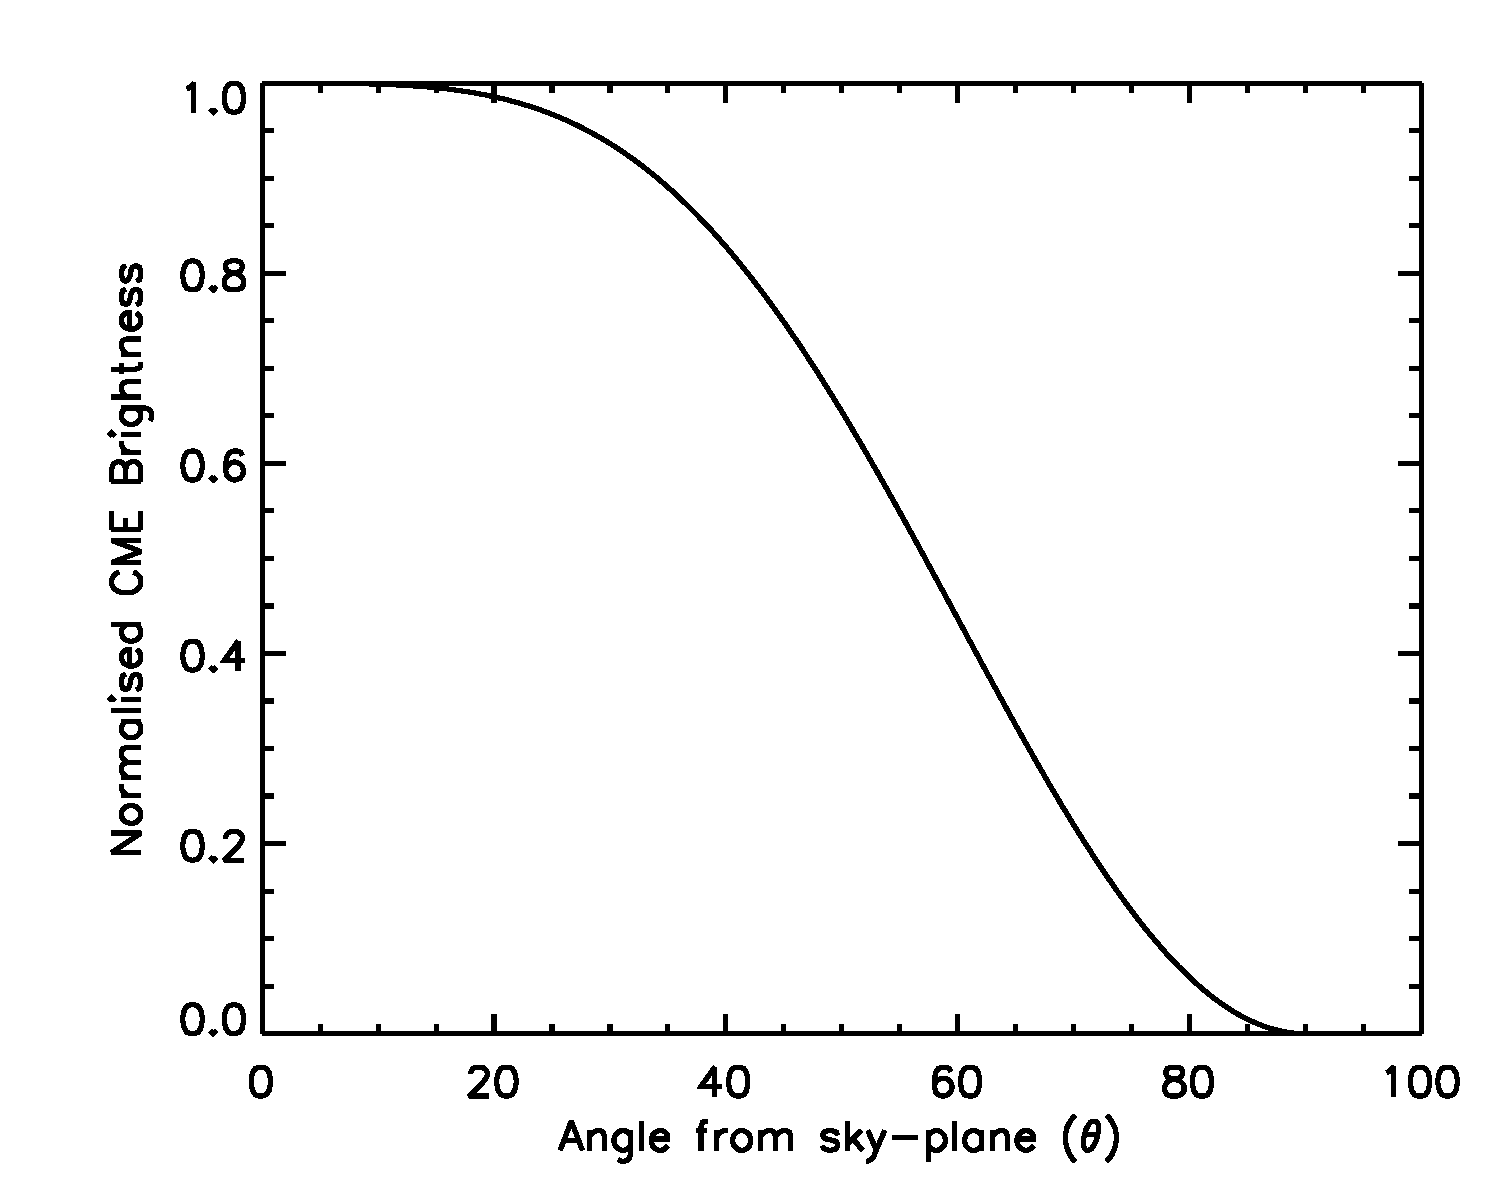
\includegraphics[scale=0.4, trim=2cm 0cm 0cm 0cm]{pos_angle.pdf}
\caption[Electron brightness as function of angle]{Normalized 2D CME brightness as a function of elongation.}
\label{fig:pos_angle}
\end{center}
\end{figure}
%------------------------------------------------------------%
%
%				     Finite Width	 				  %
%
%------------------------------------------------------------%
The second most significant assumption is that all CME material lies on a 2D plane. This assumption arrises from the fact that we do not know the distribution of CME material along the line of sight. since the 3D extent of the CME is unknown it is also assumed that the CME is confined to the 2D sky plane. In order to quantify this, we follow the method of \citep{vou00}. This simulates the brightness of a CME with homogeneous density distribution and finite angular width $\phi$ along the LOS. The simulated brightness of the CME is used to calculate a simulated observed mass by assuming that all the brightness is from electrons on the sky plane. This simulated observed mass is then compared to the actually mass as a function of CME height and radius (Figure~\ref{fig:ang_width_error}).
\begin{figure}[!t]
\begin{center}
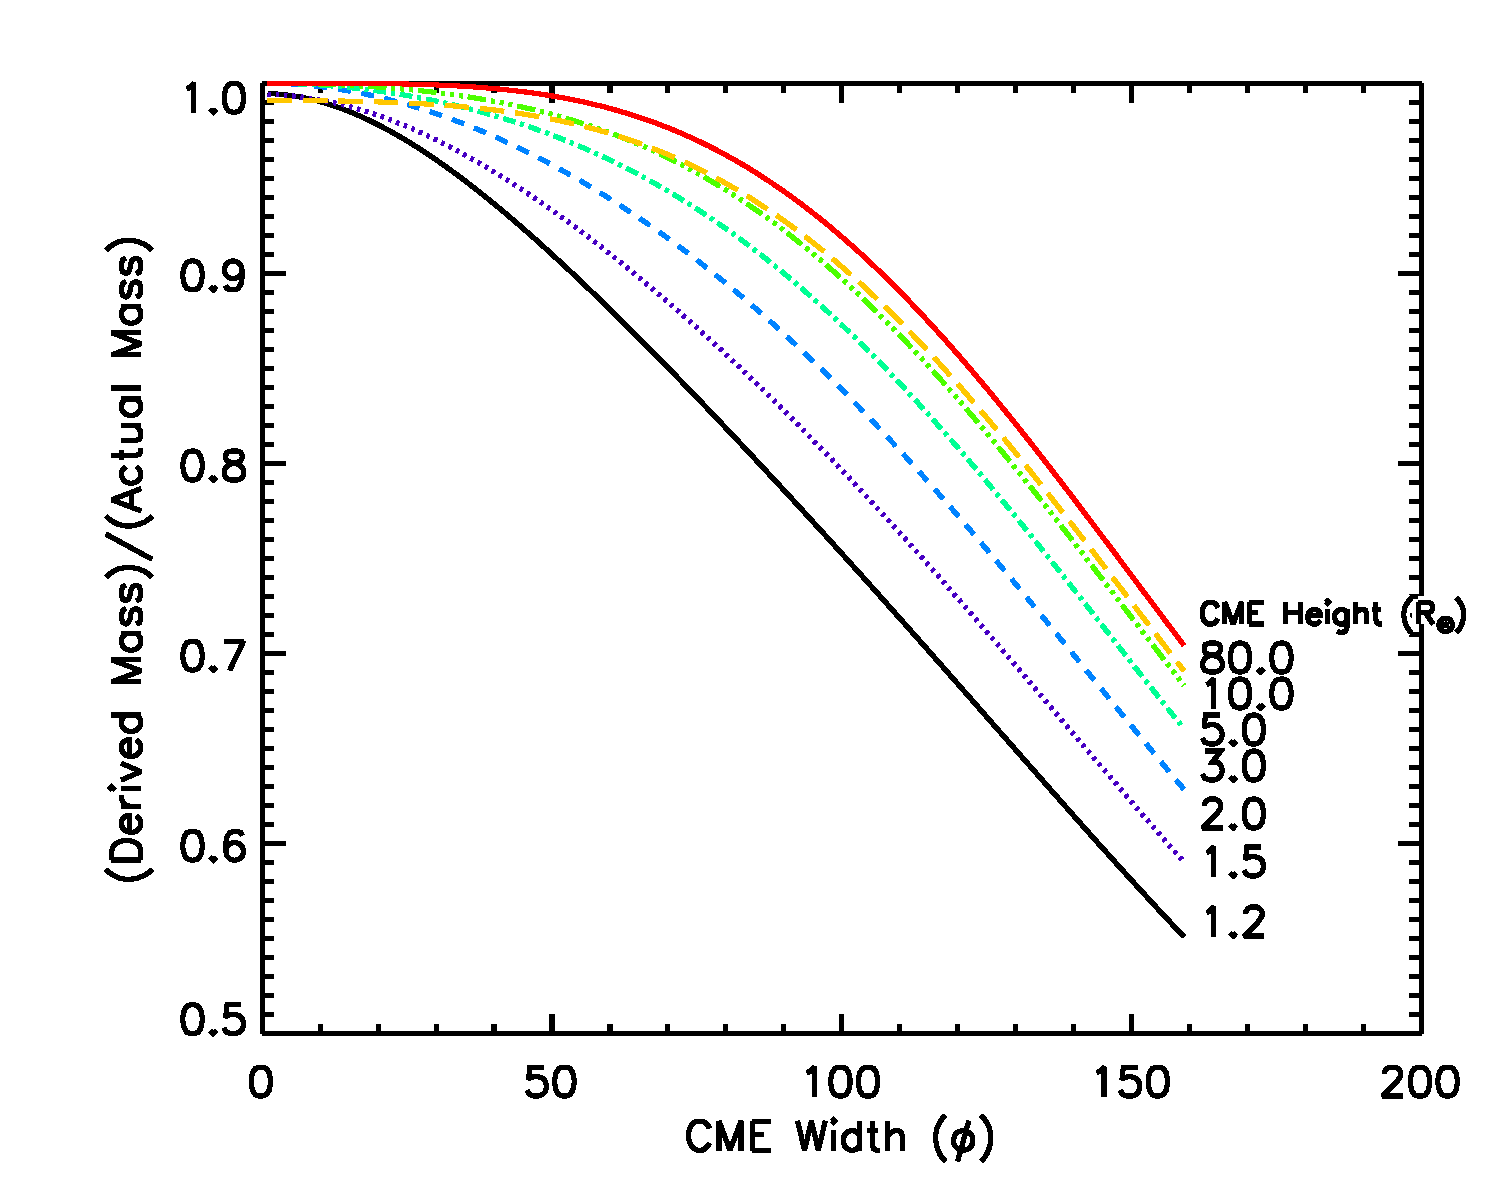
\includegraphics[scale=0.4, trim=1cm 1cm 0cm 1cm]{angular_width.pdf}
\caption[Uncertainty due to CME angular width]{Uncertainty due to CME angular width}
\label{fig:ang_width_error}
\end{center}
\end{figure}
For example, our assumption is that all CME material lies on the POS. However, the CME is centered on the sky-plane with angular width of $100^{\circ}$ and a height of $10\,R_{\odot}$. We will derive a mass of $\sim$0.9 of the actual mass. The mass underestimation from unknown angular width is smaller than the unknown plane of sky angle. However it can be significant for large angular widths at small heights.

Finally, we need to take into account that the CME will be propagating at some angle with respect to the POS \emph{and} have a finite angular width. To estimate the effects of this, we need to simulate a CME at central position angle $\theta$ and width $\phi$. We derive the simulated observed mass, given the assumption that the CME is on the sky-plane, and also the assumption that the CME material is in a 2D plane at $\theta$. 
\begin{figure}[!ht]
\begin{center}
\includegraphics[scale=0.9, angle=270, trim=1.5cm 6cm 0.4cm 0cm]{deprojected_pos.eps}
\caption{Underestimation of CME mass as a function of angle from the plane of sky. The colors correspond to a CME of angular width $\phi$. Three different heights are shown. The dashed lines are mass underestimation assuming the CME has zero width ($\phi=0$) on the POS ($\theta=0$), when in fact it is has finite width of $\phi$ and is located at $\theta$ from POS. The solid lines account for the plane of sky angle $\theta$ (they are deprojected). De-projection improves the mass underestimation up to $\theta=60^{\circ}$, after which it severely overestimates the CME mass.}
\label{fig:deprojection}
\end{center}
\end{figure}
\clearpage

This simulation is shown in Figure~\ref{fig:deprojection}, where the derived mass is compared to actual CME mass as a function of plane of sky angle. The dashed lines are the derived mass assuming that the CME has no angular width ($\pi=0^{\circ}$) and is on the sky-plane ($\theta=0^{\circ}$), when in fact it has finite width $\phi$ and is located at some $\theta >0$ (x-axis). The solid lines are derived mass assuming the CME lies on a 2D plane at the plane of sky angle $\theta$, this is called a 'de-projection' of the CME from the POS to its propagation plane at $\theta$. For example, if the CME is at a height of $5\,R_{\odot}$, has a position angle of $40^{\circ}$, and an angular width of $120^{\circ}$, but we assume it has no width (2D) and is located on the sky-plane ($theta=0^{\cric}$), then its derived mass will be 0.6 times the actual mass (underestimate of 40\%). If the CME is deprojected (we account for its sky-plane angle), then the derived mass is improved to a factor of 0.8 of the actual mass. Note that de-projection still assumes the CME has no width ($\phi=0$), hence there is still a mass underestimation after de-projection.

There is an interesting point at $\sim$$\theta=55^{\circ}$ for the $5\,R_{\odot}$ and $10\,R_{\odot}$ plots (and all larger heights). For all angular widths $\phi$, a deprojection will derive exactly the actual CME mass. Beyond this point, de-projection starts to over-estimate the CME mass and eventually overestimates it by a severe estimate at sky-plane angle greater than $70^{\circ}$. As we will see, the CME in this study had a POS angle of $45^{\circ}$ and an angular width no greater than $120^{\circ}$ for the height range of 1.4--12$R_{\odot}$. Therefore, as shown in Figure X, it is better to deproject the CME brightness to its propagation plane, as this underestimates the mass by a smaller factor than assuming the CME is on the POS.


%---------------FROM HERE---------------------------%

The CME of 2008 December 12 was Earth-directed \citep{byr10}, making it roughly the same angular distance from both the \emph{STEREO}\,A\,and\,B spacecraft, then located $\pm$45 degrees from Earth. This known angle of propagation was used to convert from pixel values of MSB to grams via the expression
\begin{equation}
m_{pixel}=\frac{B_{obs}}{B_{e}}\times1.97\times10^{-24}\,\mathrm{g}
\end{equation}
where $B_{obs}$ is the observed MSB of the pixel, $B_{e}$ is the electron brightness calculated from the van de Hulst coefficients, and 1.97$ \times10^{-24}$\,g is a factor that converts the number of electrons to mass, assuming a completely ionized corona with a composition of 90\% hydrogen and 10\% helium. The known angle of propagation allowed the correct value of $B_{e}$ to be computed resulting in a significant reduction in the uncertainties associated with the propagation angle. The largest remaining uncertainty is the unknown angular width along the LOS. This uncertainty was quantified in a similar approach to the method outlined in \citet{vou00}. This simulates the brightness of a CME with 
homogeneous density distribution and finite angular width along the LOS--longitudinal angular width $\Delta$$\theta_{long}$, allowing calculation of a simulated observed mass. Comparing this to the actual mass allowed for an evaluation of CME mass underestimation for given values of $\Delta$$\theta_{long}$.  Since the values for $\Delta$$\theta_{long}$ are unknown, the expression derived in \citet{byr10} for the \emph{latitudinal} 
angular width of this CME as a function of height, $\Delta$$\theta_{lat}$$(r)=25r^{0.22}$, was used to define an upper limit to $\Delta$$\theta_{long}$. It was assumed the CME longitudinal angular width is no more than twice the latitudinal angular width, or $\Delta$$\theta_{long}$$\leqslant$\,2$\times$$\Delta$$\theta_{lat}$. Such an upper limit is in agreement with simulations of flux-rope CMEs which give a typical aspect ratio of broadside to axial angular extents of 1.6\,--\,1.9 \citep{krall2006}. Hence the value for $\Delta$$\theta_{long}$ at each height was used to obtain the simulated mass underestimation estimates described above. The heights and angular widths used in this study produced CME mass underestimation estimates of between 5--10\% for finite angular width uncertainty. An extra mass uncertainty of 6\% was added to account for the assumption of coronal abundance of 90\% hydrogen and 10\% helium which can lead to slight errors while converting from pixel values of MSB to grams \citep{vour2010}. 

%-----------------------------%


To calculate the CME mass a user-selected area (the extent of the CME, for example) of the base difference image was chosen and the pixel values within this area were summed to obtain total mass. Figure~\ref{fig:STEREO_COR2A&B} COR2 B images show an example of the sector over which pixels were summed (the smaller sectors indicate a different summing region used at a later stage). The selected area was chosen for each image in the time sequence of CME propagation so as to determine the mass variation with height in COR1 and 2 using both A and B. The selection of an area by a point and click method is of course a subjective identification of the the extent of the CME, 
so it is susceptible to user-generated uncertainties. To quantify these uncertainties the mass was obtained for each coronagraph image in the time sequence (as described above) and the process was repeated five times in order to obtain the mean CME mass for each image and the standard error on the mean. This standard error was defined as the uncertainty due to user bias in the point and click method of CME identification. The height at each measurement interval was taken to be the heliocentric distance of the CME apex in the image i.e., the apex of the front was chosen 
by simple point-and-click method. The uncertainty on the apex height was also found by the standard error on five runs.


The deflection of a small streamer during CME propagation produces negative pixels in the base difference images. The effect is particularly apparent in the COR1 images, Figure~\ref{fig:STEREO_COR1A&B}. It is difficult to unambiguously distinguish between streamer and CME, making it difficult to quantify the uncertainty introduced due to streamer interaction. To make an estimate of the streamer's effects, a calculation of its mass in the pre-event image was made. A number of different samples of the area of the streamer in the COR1\,B pre-event image that effects all subsequent images produced a mass estimate of $\sim$5$\times$10$^{14}$\,g. This mass was used as a measure of the uncertainty introduced due to streamer interaction in the COR1\,B images. A similar analysis of the COR1\,A pre-event images gave a streamer mass estimate of $\sim$7$\times$10$^{14}$\,g. COR2 images are relatively unaffected by significant changes in background coronal brightness and do not suffer from negative pixel values to as large an extent as COR1. The pre-event image of COR2\,B is particularly clean and free of background streamers, hence COR2\,B images are considered to provide most accurate CME mass estimation.

Finally, in order to obtain a more complete and continuous estimate of CME mass growth, the masses determined from both COR1 and COR2 coronagraphs were summed in those cases where image times of the inner and outer coronagraphs overlapped\footnote{A difference in cadence of the inner and outer coronagraphs means that the images closest in time have a three minute offset e.g., a COR1 image taken at 07:25 UT was considered to be coincident in time with the COR2 image at 07:22 UT}. The overlap in the inner and outer corongraphs' fields of view was also taken into account in this summation.


A concise measurement of the CME kinematics, such as velocity and acceleration, were taken from the results of the study of \citet{byr10}. Since these kinematics take into account the true three dimensional surface of the front they provide reliable estimates of CME velocity and acceleration in 3-D space. These velocity and acceleration measurements were used in the calculation of kinetic energy and total force on the CME for each point in time. The CME mass used in all energy and force calculations was the asymptotic mass it approaches at later stages of its evolution beyond 10\,$R_{\odot}$ as observed from the \emph{STEREO B} spacecraft i.e.,\,3.4\,$\pm$\,1.0$\times$10$^{15}$\,g. As will be shown, there is 
good motivation for the use of constant mass in the magnitude of kinetic energy and force estimates. 


\section{Results}\label{sec:11}
\subsection{Masses}

The results of the calculation for CME mass development with time and height for both \emph{STEREO} A and B coronagraphs are shown in Figure~\ref{fig:20081212_mass_ht}. In panel (a), the height values are those taken from a point-and-click method of tracking the CME apex; these heights are corrected for CME propagation angle of $\sim$$45^{\circ}$.  In both panels (a) and (b), the mass estimates of \emph{STEREO} A and B follow a similar trend and have similar values at each stage in the propagation. Such good agreement between mass values is a good indicator that $\sim$$45^{\circ}$ is the correct angle of propagation from the sky-plane. A change in the cadence of mass measurements is noticeable at $\sim$08:00 UT (or $\gtrsim$5\,$R_{\odot}$). This is due to the use of only COR1 images (with a cadence of 10\,minutes) prior to this time, and the use of the COR2 plus COR1 images after this time (the cadence of these measurements follows that of COR2\,--\,30\,minutes). Comparing A and B below 4.5\,$R_{\odot}$, mass values show a similar trend and increase at the same rate, but at approximately 3\,$R_{\odot}$ the mass measurements in COR1\,B appear to increase to a much larger value then fall again. This effect is visible in the COR1\,A measurements, albeit 
diminished. It is probably due to the presence of a prominence which contains a significant mass content and therefore contributes a large amount to total measured CME mass. Also, early on in its propagation, the prominence may still be emitting H-$\alpha$ line radiation (656.28 nm) due to the larger fraction of neutral hydrogen at its cooler temperatures.
\begin{figure}
\begin{center}
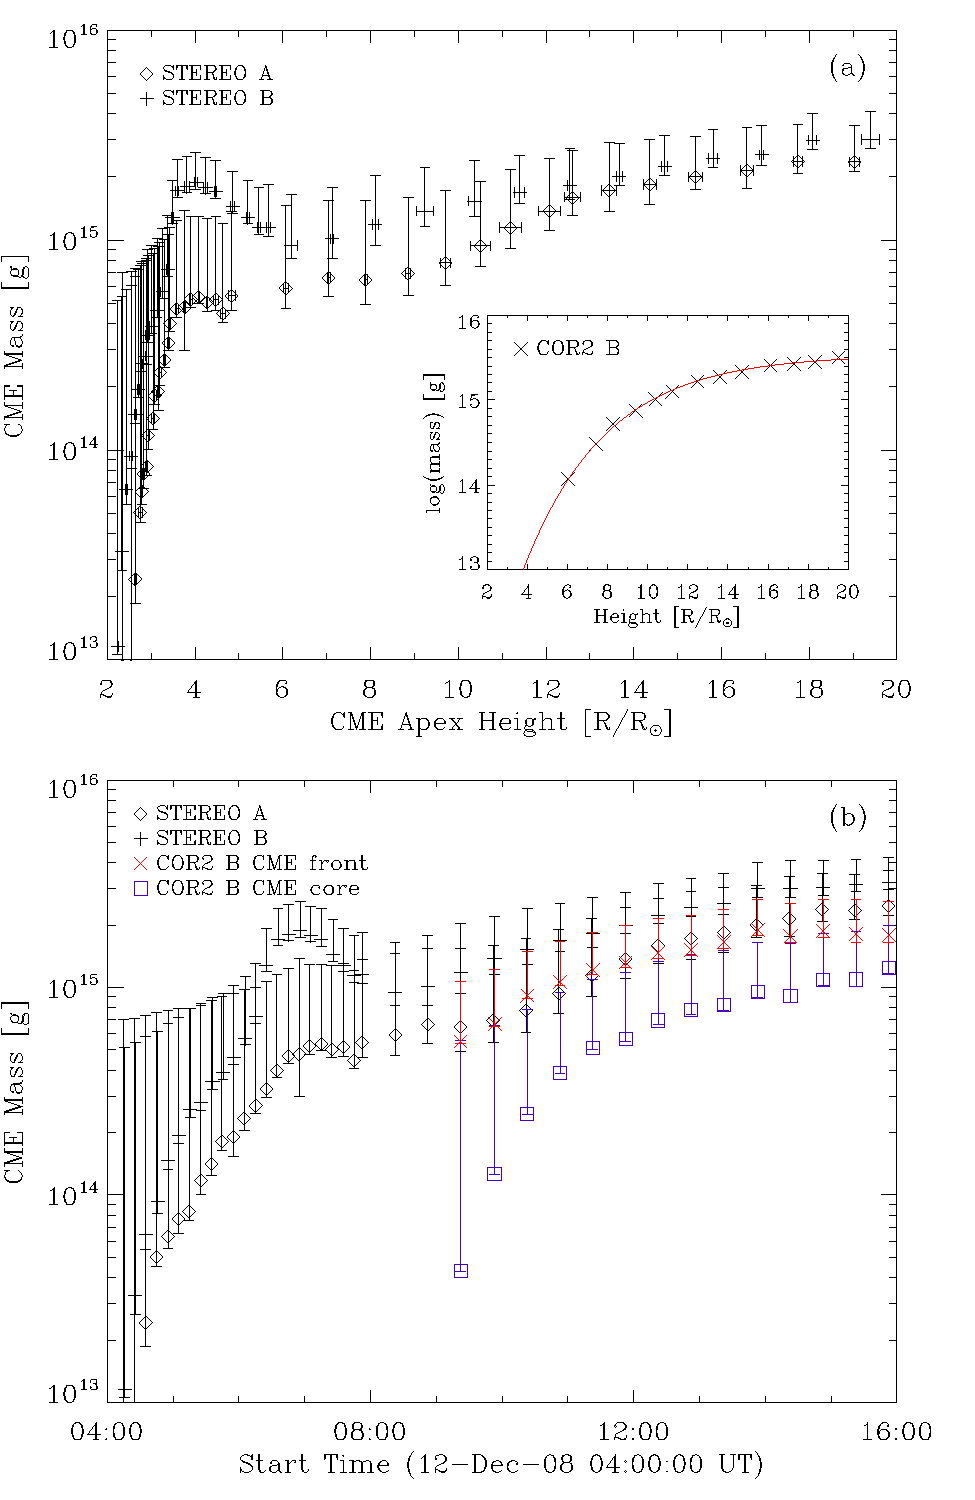
\includegraphics[scale=0.7, angle=0]{20081212_mass_ht.pdf}
\caption[CME mass as a function of height and time]{CME mass development with height (a) and time (b), for the 2008 December 12 CME. After $\sim$08:00 UT ($\gtrsim$5\,$R_{\odot}$) the 
masses from the inner and outer coronagraphs are summed to show uninterrupted 
mass development from $\sim$2--20\,$R_{\odot}$ over a period of 12 hours. The small bump in the 
CME mass at $\sim$07:00\,UT ($\sim$4\,$R_{\odot}$) is probably due to an unknown amount of H-$\alpha$ emission from the prominence. Mass of 
CME front and core are also shown, red $\textquoteleft$$\times$' and blue square, for COR2\,B, panel (b). After 14:52\,UT they share approximately 
equal mass. The inset of (a) shows mass development with height for COR2\,B only; the red curve represents a fit to the data whereby the mass 
asymptotically approaches $3.4\,\pm\,1.0\times10^{15}$\,g. }
\end{center}
\label{fig:20081212_mass_ht}
\end{figure}
\clearpage
The COR1 imaging passband is centered on H-$\alpha$ so any emission in the prominence from neutral hydrogen could be contributing to light received by the COR1 coronagraphs, this is apparent from the saturation region in the COR1\,B images in Figure~\ref{fig:STEREO_COR1A&B}. Since this is resonance line emission, and not Thomson scattered emission, it leads to an erroneous measurement in CME mass. Thus, it is assumed the larger rise and fall in 
CME mass is caused by the prominence entering and exiting the COR1\,B field of view. The effect is diminished in COR1\,A since the prominence does not enter the FOV to as large an extent as in COR1\,B. The interpretation that the $\textquoteleft$mass bump' is not actual mass growth (or loss) is supported by previous measurements where CME mass increase follows a trend with height described by $M_{cme}(h)=M_{a}(1-e^{-h/h_a})$, where $M_a$ is the final mass the CME approaches asymptotically and $h_a$ is the height at which the CME reaches 0.63$M_a$ \citep
{cola09}, with no  $\textquoteleft$bump'~in mass earlier on. The decline in mass after the peak may be explained by the ionization of neutral hydrogen such that H-$\alpha$ emission diminishes and simply becomes Thomson scattering of free electrons, as with the rest of the CME material. 

In order to produce a fit to the data, the COR2\,B mass results were chosen because its pre-event image was largely free of any bright streamers or other features which introduce unwanted effects in the production of base difference images, as described above. A fit with the above equation resulted in a final asymptotic CME mass of 3.4\,$\pm$\,1.0$\times$10$^{15}$\,g, with a scale height of $h_a=2.9\,R_{\odot}$. This fit is plotted along with the COR2\,B data in the inset panel of Figure~\ref{fig:20081212_mass_ht}(a). Note that the mass increase is due to material coming up from below the occulting disk, and not actual mass gain of the CME. The uncertainty on the above asymptotic mass value was taken to be 30\%, from the largest uncertainty  due to finite width, the conversion factor uncertainty as described above, the standard error user-generated uncertainty, and uncertainty due to streamer interaction.

In each image where the CME core and front are distinguishable, their masses were measured separately. This was regions demarcating the areas of core and front, see COR2\,B at 12:22\,UT and 14:52\,UT in Figure~\ref{fig:STEREO_COR2A&B} for an example of the separate core and front sectors over which pixel values were summed to obtain total mass. The uncertainties due to finite width of the observed object also apply to the core and front measurements, however, since the widths of these particular areas of the CME are unknown we chose the maximum uncertainty of 10\% from the above analysis since neither core nor front can be any wider than the maximum width assigned to this CME. The remaining uncertainties described above were also applied. The mass development of core and front with time is shown in Figure~\ref{fig:20081212_mass_ht}(b). The two mass measurements are subject to an observational effect of apparent exponential mass growth, however by the time the CME is fully in the field of view 
at 14:45\,UT the core and front share approximately equal mass. 


\subsection{Energies}\label{sec:2}

In the following calculations, all measurements of force and kinetic energy use the asymptotic mass of 3.4\,$\pm$\,1.0$\times$10$^{15}$\,g and not the instantaneous mass values calculated from each coronagraph image i.e., the CME is considered to begin its propagation with this mass and does not acquire any mass as it propagates. 

Estimates of the force and kinetic energy use the 3-D velocity and acceleration measurements produced by \citet{byr10}. Their method firstly identifies the CME front in each coronagraph image using a multiscale edge detection filter. The front edges were then used to define a quadrilateral in space into which an ellipse is fit, this method is known as elliptical tie-pointing. This was done for multiple horizontal planes through the CME so that the fit ellipses outline a curved front in 3-D space.The speed and acceleration were then deduced from the change in position of the front, with time, through the \emph{STEREO} COR1, COR2 and HI fields of view. Since mass measurements in this study use only the COR1 and COR2 coronagraphs, HI kinematics measurements have been excluded here. The CME front position uncertainty in \emph{STEREO A}\,and\,\emph{B} coronagraphs was determined from the filter width in the multiscale analysis. Velocity and acceleration uncertainties were then propagated from position uncertainty.  Figure~\ref{fig:force_20081212}(a) shows CME velocity as a function of heliocentric distance, along with acceleration in panel (b). 

\begin{figure}[h!]
\begin{center}
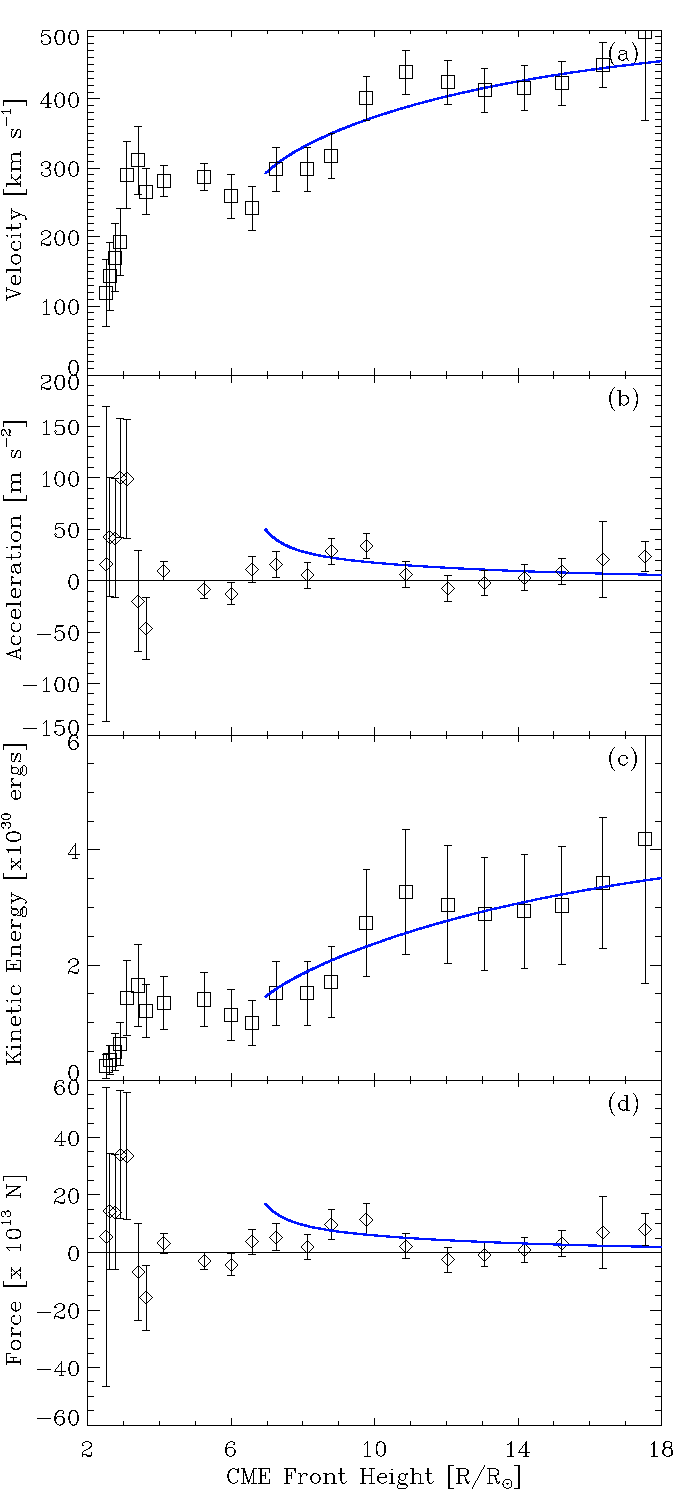
\includegraphics[scale=0.75, angle=0]{images/20081212_force_v2.pdf}
\caption[CME kinematics and energetics as a function of height]{(a) CME velocity as a function of heliocentric distance, including a fit to the data produced using an aerodynamic drag model beyond $\sim$7\,$R_{\odot}$ \citep{byr10}. (b) Acceleration of CME, including fit,  derived from the velocity data and fit. 
Panel (c) and (d) show the kinetic energy and force, respectively, both calculated using constant CME mass of $3.4\,\pm\,1.0\times10^{15}$\,g and kinematics results from (a) and (b). Also shown are the fits to energy and force produced from fits to velocity and acceleration.}
\end{center}
\label{fig:force_20081212}
\end{figure}
\clearpage

The CME kinetic energy was calculated using $E_{kin}=1/2M_{cme}v_{cme}^{2}$, where $M_{cme}$ is the final asymptotic mass of 3.4\,$\pm$\,1.0$\times$10$^{15}$\,g and $v_{cme}$ are the instantaneous velocity measurements, results of this calculation are shown in Figure~\ref{fig:force_20081212}(c). The kinetic energy shows 
an initial rise towards 6.3\,$\pm$\,3.7$\times$10$^{29}$\,ergs at $\sim$3\,$R_{\odot}$, beyond which it rises steadily to 4.2\,$\pm$\,2.5$\times$10$^{30}$\,ergs at $\sim$18\,$R_{\odot}$, these values are similar to those reported in \citet{vou00,vour2010} and \citet{emslie2004}. 

The total force on the CME was calculated using $F_{total}=M_{cme}a_{cme}$, where $M_{cme}$ is as above and $a_{cme}$ is taken from the instantaneous acceleration values. As shown in panel (d) of Figure~\ref{fig:force_20081212}, the force initially grows significantly, reaching a maximum value of 3.4\,$\pm$\,2.2$\times$10$^{14}$\,N at $\sim$3\,$R_
{\odot}$. The early rise and fall in acceleration (or force) is in agreement with a previous study of a CME observed to reach peak acceleration at $\sim$1.7\,$R_{\odot}$ after which it reaches a constant velocity beyond $\sim$3.4\,$R_{\odot}$ \citep{gallagher03}.  Such results are also found in a statistical study which shows that the majority of CMEs have peak acceleration in the low corona with a mean height of maximum acceleration at 1.5\,$R_{\odot}$ 
\citep{bein2011}. Similarly, observational studies by \citet{zhang2001} and \citet{zhang2004} also show early phase peak acceleration between 2--5\,$R_{\odot}$ and forces on the order of 10$^{15}$\,N and 10$^{12}$\,N, depending on whether the CME shows large initial acceleration or a slow, more gradual acceleration.

After this early peak, the force drops to an average value of 3.8$\pm$5.4$\times$10$^{13}$\,N at distances between 7--18\,$R_{\odot}$. It is apparent from Figure~\ref{fig:force_20081212}(a) that the velocity continues to increase beyond $7\,R_{\odot}$, implying that a positive radial force must be present. To clarify this, a fit to the velocity data using a model for solar wind drag on the CME beyond $7\,R_{\odot}$ (as outlined in \citet{byr10}) is shown in Figure~\ref{fig:force_20081212}(a). Although the data suggest a non-monotonic increase in velocity, the fit reveals that propagation is best described by a steadily increasing velocity between 7--18\,$R_{\odot}$. The acceleration and kinetic energy curves derived from this velocity fit are shown in Figure~\ref{fig:force_20081212}(b) and (c). In Figure~\ref{fig:force_20081212}(d), the curve for the force derived from the velocity fit initially deviates from the data at $\sim$7\,$R_{\odot}$, however beyond this distance there is good agreement with the data and the derived force is entirely positive.  This suggests that the solar wind exerts a positive aerodynamic drag force on the CME, resulting in a velocity that approaches the asymptotic solar wind speed at large heliospheric distances. 

%\subsection{Mechanical Energy}\label{sec:20}

\subsection{Forces}\label{sec:21}

It should be noted that Figure~\ref{fig:20081212_mass_ht} shows an overall exponential increase in CME mass with height which could be interpreted as the CME rapidly gaining mass as it propagates. Care should be taken with this interpretation since this apparent exponential mass increase is almost certainly due to the CME moving into the field of view, therefore allowing us to measure more of its mass content; such an interpretation is in agreement with similar assertions made in \citet{vour2010}. It is difficult to distinguish between actual CME mass growth and an apparent growth due to more of the CME being observed. If the initial early rise in CME mass is assumed to be an observational artifact then we can interpret the CME mass to be in the range of (3--3.5)$\times$10$^{15}$\,g for most of its early propagation i.e., the CME already has such a mass before launch and does not acquire more mass (via inflows or otherwise) during propagation.
Such an interpretation is in agreement with CME mass measurements calculated from dimmings in \emph{STEREO} Extreme Ultraviolet Image(EUVI) images, which show the mass calculated from EUV images to be approximately equal to CME mass in COR2 images,  $m_{EUVI}/m_{COR2} =1.1\pm0.3$  \citep{aschw09}. Once the CME bubble is in the field of view at $\sim$10\,$R_{\odot}$ the mass in its entirety can be measured and the increase beyond this point, if any, is slow and steady, Figure~\ref{fig:20081212_mass_ht}.

The early stages of CME propagation are dominated by a sharp rise to a peak force of 3.4\,$\pm$\,2.2$\times$10$^{14}$\,N at $\sim$3\,$R_{\odot}$ followed by a sharp decline, Figure~\ref{fig:force_20081212}(d). The catastrophe model \citep{forbes1991,forbes1995,lin2000}, magnetic breakout model \citep{antio99,lynch2008}, and toroidal instability model \citep{chen1996,kleim2006} employ a number of forces acting on the CME to produce an over all acceleration into interplanetary space. For example, the toroidal instability model used by \citet{chen1996} uses a Lorentz hoop force (or Lorentz self-force), solar wind drag, and gravity to provide a net force acting on the CME between 2--3\,$R_{\odot}$ that quickly 
rises to a peak total force of $\sim$10$^{16}$\,N and then falls rapidly.

If we assume that the peak force observed for the 2008 December 12 CME is the net force due to similar forces used in the above models, such as the solar wind drag, gravity, and some form of magnetic CME driver e.g., a $\vec{J}\,\times\,\vec{B}$ force, we may estimate their relative contribution. The force due to solar wind drag on the CME is given by
\begin{equation}
\vec{F}_d=-\frac{1}{2}C_{d}\rho_{sw}A_{cme}(\vec{v}-\vec{v}_{sw})\mid\,\vec{v}-\vec{v}_{sw}\mid
\end{equation}
where $M_{cme}$ is the CME mass, $\vec{v}$ is the CME velocity, $C_{d}$ is the drag coefficient, $\rho_{sw}$ is the solar wind mass density, $A_{cme}$ is the CME area exposed to solar wind drag and $\vec{v}_{sw}$ is the solar wind velocity \citep{malo10}. To estimate the effects of this force we use $\rho_{sw}=n_{p}m_{p}$, where $m_{p}$ is proton mass, and assume ionization fraction of $\chi$\,=\,1 such that $n_{p}=n_{e}$\,$[cm^{-3}]$. Electron density, and hence proton density, is then given by an interplanetary density model derived from a special solution of the Parker solar wind equation \citep{Mann1999}, solar wind velocity values as a function of height are also determined using this model. $A_{cme}$ is estimated using the expression derived in \citet{byr10} for latitudinal angular width of the CME as a function of height, $\Delta$$\theta_{lat}$$(r)=26r^{0.22}$. This is used to derive an arc length of the CME front and, as above, making the assumption $\Delta$$\theta_{long}$$=$\,2$\times$$\Delta$$\theta_{lat}$, the two arc lengths derived from these angles then give the surface that the solar wind acts on, thus $A_{cme}$\,=\,1352$r^{2.44}$. Setting the drag coefficient $C_{d}=1$, and using the \citet{Mann1999} model to derive a density and a solar wind velocity of 2.3$\times$10$^{5}$\,cm$^{-3}$  and 70\,km\,s$^{-1}$, respectively, equation [1] then gives a force of $\vec{F}_{d}=-8.0\times10^{12}\,\hat{r}\,$\,N for solar wind drag at $\sim$3\,$R_{\odot}$, where $\hat{r}$ is a unit vector in the positive radial direction. 

A simple estimate of force due to gravity is given by $\vec{F}_{g}=GM_{\odot}M_{cme}/\vec{r}\,^2$, where $G$ is the universal gravitational constant, $M_{\odot}$ is solar mass, $M_{cme}$ is CME mass, and $\vec{r}$ is a heliocentric position vector\footnote{Ideally the heliocentric distance of the CME centre of mass would be used here. However an unknown amount of mass is obscured by the coronagraphs occulting disk, making the mass distribution and hence COM difficult to determine. Thus the CME front height is used in the calculation of force due to gravity}. Given a CME mass of 3.4$\times$10$^{15}$\,g the force due to gravity at a heliocentric distance of 3\,$R_{\odot}$ is $\vec{F}_{g}=-1.0\times10^
{14}\,\hat{r}$\,N. The only remaining contribution is due to some form of magnetic CME driver, $F_{mag}$, which is estimated using 
\begin{equation}
\vec{F}_{mag}= \vec{F}_{total}-\vec{F}_{d}-\vec{F}_{g}
\end{equation}
(the pressure gradient in the CME equation of motion is assumed to be negligable and has been omitted here). Using the above values, the total magnetic contribution to CME force is calculated to be $\vec{F}_{mag}\approx4.5\times10^{14}\,\hat{r}$\,N at 3\,$R_{\odot}$, indicating that this is the largest driver of CMEs at low coronal heights. Lorentz force dominated dynamics in early phase CME propagation are reported in \citet{bein2011}, in which a statistical study of a large sample of CMEs in EUVI, COR1, and COR2 indicated an early phase acceleration for the majority of CMEs that is attributable to a Lorentz force.  A similar result of an observational study by \citet{vrs06} found that the Lorentz force plays a dominant role within a few solar radii. It should be noted that although we have labelled the force $F_{mag}$, there is no distinction on the exact form of this force e.g., whether it is magnetic pressure, magnetic tension, or a Lorentz self-force that acts as the driver. Also, any non-radial motion of the CME, such as that described in \citet{byr10}, is not taken into account here; any force estimates are purely radial in direction.


 \section{Conclusion} \label{bozomath}
 The \emph{STEREO} COR1/2 coronagraphs have been used to determine the mass development of the 2008 December 12 CME. Knowledge of the longitudinal propagation angle of the CME allowed for a significant reduction in the mass uncertainty, giving a final estimate of 3.4\,$\pm$\,1.0$\times$10$^{15}$\,g. Using kinematics results of a previous study \citep{byr10}, the velocity and acceleration of the CME were combined with the mass measurements to determine the kinetic energy and total force on the CME. The early phase propagation of the CME was found to be dominated by a force of peak magnitude of 3.4\,$\pm$\,2.2$\times$10$^{14}$\,N at $\sim$3.0\,$R_{\odot}$, after which the magnitude declines 
rapidly and settles to and average of 3.8 $\pm$ 5.4$\times$10$^{13}$\,N. This early rise and fall in total force (or acceleration) is in agreement with previous observations of CME kinematics \citep{gallagher03, bein2011}. Similarly results of observational studies by \citet{zhang2001} and \citet{zhang2004} also show early phase peak acceleration between 2--5\,$R_{\odot}$ and forces on the order of 10$^{15}$\,N and 10$^{12}$\,N. The kinetic energy shows an initial rise steadily to 4.2\,$\pm$\,2.5$\times$10$^{30}$\,ergs at $\sim$18\,$R_{\odot}$, such order of magnitudes are similar to those reported in \citet{vou00,emslie2004} and are typical of CME kinetic energies \citep{vour2010}.

Such CME kinematics and dynamics property estimates cannot be carried out when unknown propagation angle hinders an accurate calculation of CME mass, hence adding unacceptable uncertainty to any subsequent calculations. This highlights the need for similar studies using the \emph{STEREO} mission's ability to accurately determine the physical properties of CMEs, such as mass, with remarkably reduced uncertainty. Increasing the accuracy of force estimates of other well studied CMEs will allow for a more complete view of the magnitude of the forces influencing CME propagation and will allow model parameters to be more accurately constrained.





%!TEX root = ../thesis.tex
%Adding the above line, with the name of your base .tex file (in this case "thesis.tex") will allow you to compile the whole thesis even when working inside one of the chapter tex files
\vspace{-5mm}
\singlespacing
\chapter{Coronal Mass Ejection Shocks and Particle Acceleration} 
\label{chap:5}
\doublespacing
\vspace{-10mm}
CMEs often erupt at speeds in excess of the local magnetoacoustic wave speeds in the corona. Traveling in excess of Alfv\'{e}n Mach 1, they often drive shocks which can have a variety of physical manifestations, such as radio bursts, coronal bright fronts (CBFs), white-light enhancements, and the in-situ detection of energetic particles. Despite such a variety of shock phenomena being observed for decades, the unifying physical mechanism between these phenomena remains unknown. This chapter will provide an analysis that uses extreme ultraviolet, radio, and white-light imaging of an eruptive event on 22 September 2011 to determine the properties of a CME-driven shock in the corona. The results show that a plasma shock with an Alfv\'{e}n Mach number of $2.4^{+0.7}_{-0.8}$ was coincident with a coronal bright front and an intense metric radio burst generated by electrons with kinetic energies of 2--46 keV. This work provides new evidence to show that the relationship between CMEs, CBFs, and radio radio bursts can be a coronal shock driven by the CME flank. The chapter is based on publications by Carley et al., {\it Nature Physics}, 2013, and Zucca et al., {\it Astronomy \& Astrophysics}, submitted.

\doublespacing
\section{Introduction}\label{sec:1}
Coronal mass ejections (CMEs) 
%are spectacular eruptions of magnetized plasma from the low solar atmosphere into interplanetary space \citep{byrne2010, roussev2012}. With kinetic energies of $\sim$$10^{25}$\,J \citep{vour2010}, they are the most energetic explosive events in the solar system and 
are often associated with plasma shocks and the acceleration of particles to relativistic speeds \citep{klassen2002, grechnev2011}. However, the underlying mechanism relating CMEs, shocks, and particle acceleration is still a subject of intense debate \citep{vrsnak2008}. By clarifying the inherent characteristics of these phenomena we learn not only about the nature of explosive plasma events but also about how they drive shocks and accelerate particles to high energies. The understanding of such processes are important for fundamental solar physics, plasma physics, and space weather predictions.

%ubiquitous in the universe, playing a role in the acceleration of cosmic rays in supernovae and active galactic nuclei shocks \citep{drury2012}.


CME-associated shocks are often observed over a variety of spectral bands. At radio frequencies, high intensity ($\sim$$10^8$\,Jy) emissions, known as type II and type III bursts, are associated with coronal shocks and accelerated particles in the solar corona \citep{wild1950, mann1996}. Fine structure in these radio bursts can often reveal a \textquoteleft bursty' nature to the shock particle acceleration \citep{mann2005}, which can reveal details of the internal shock structure \citep{zlobec1993, guo2010}.
At extreme ultraviolet (EUV) wavelengths, the shock or pressure pulse response of the corona to an eruption may be imaged as a bright pulse propagating across the entire solar disk at typical velocities of 200--400\,km\,s$^{-1}$ \citep{gallagher2011}. These \textquoteleft coronal bright fronts' (CBFs) are a regular feature of solar eruptive events and often display wave-like properties such as reflection \citep{gopal2009}, refraction \citep{wang2000} and pulse broadening \citep{long2011}. %
Like CMEs, CBFs are often accompanied by type II and type III radio bursts, with EUV and radio images revealing a spatial link between the phenomena that is suggestive of a common origin \citep{maia2004, kozarev2011, vrsna2005}.


It has been proposed that the common origin for these myriad phenomena may be a CME-driven shock \citep{grechnev2011, warmuth2004b}.  In this scenario, the CME eruption drives a pressure pulse, observable in the low corona as a propagating wave-like CBF. Higher in the corona this same pulse forms a shock, accelerating particles and producing type II and III emission. However, much debate surrounds the suggestion that (i) the CBF is a plasma pressure wave driven by a CME, and (ii) the radio bursts, generated by accelerated particles, result from this same wave/shock system. The contention has arisen from attempts to explain non-wave kinematics of CBFs \citep{zhukov2009}. Pseudo-wave theories are employed to describe this behavior, where the erupting CME produces a large-scale restructuring of the coronal magnetic field, which results in a propagating bright pulse (via Joule plasma heating) that is not actually a driven wave \citep{delannee2008}. In this scenario, any relationship with shock observables is indirect. Further confusion is added by the possibility that high energy particles in association with the eruption may be a consequence of magnetic reconnection in the flaring active region, and not the result of a shock \citep{kahler2007}.

Collectively, CMEs, CBFs and radio bursts provide direct measures of both shock kinematics and the characteristics of the accompanying accelerated particles. However, a common theory explaining these phenomena has yet to be verified.
This lack of clarity can be ascribed to an EUV imaging cadence that was unable to match the fast time sampling of radio imaging and spectroscopy. Now, using the high image cadence of the Solar Dynamics Observatory \citep[SDO;][]{presnell2012}, combined with fast time sampling radio images and spectra, we can reveal previously unseen characteristics of the relationship between these phenomena, proving that a CME-driven shock is the feature unifying these observations and that this shock is responsible for bursty electron acceleration. This greatly advances our understanding of the close relationship between solar eruptions, plasma shocks and their resulting EUV, radio and particle acceleration signatures.


%----------------------------------------------------%
%			CBF and radio source		    %
%											    %	

\section{Coronal Bright Front and Radio Source}\label{sec:10}

%------------------ Observations --------------------%
\subsection{Observations}
On 22 September 2011 at 10:29\,UT, an X-ray flare (GOES class X1.4) began in an active region located on the east limb of the Sun (NOAA active region 11302; N13E78). Approximately 11 minutes after the flare start time, a bright wave-like front (CBF) was observed propagating away from the southern edge of the active region in SDO/Atmospheric Imaging Assembly \citep[AIA;][]{lemen2012} 21.1\,nm passband images. The CBF then propagated along the east limb from $\sim$15$^{\circ}\,$\,south to $\sim$50$^{\circ}\,$\,south of the equator (Figure.~\ref{fig:figure_aia_nrh_c2}). During the same period of the CBF propagation, a bright 150.9\,MHz source formed above the CBF, imaged using the Nan\c{c}ay Radioheliograph \citep[NRH;][]{kerdraon1997} (contours Figure.~\ref{fig:figure_aia_nrh_c2}). 
%
%
\begin{sidewaysfigure}
    \centering
	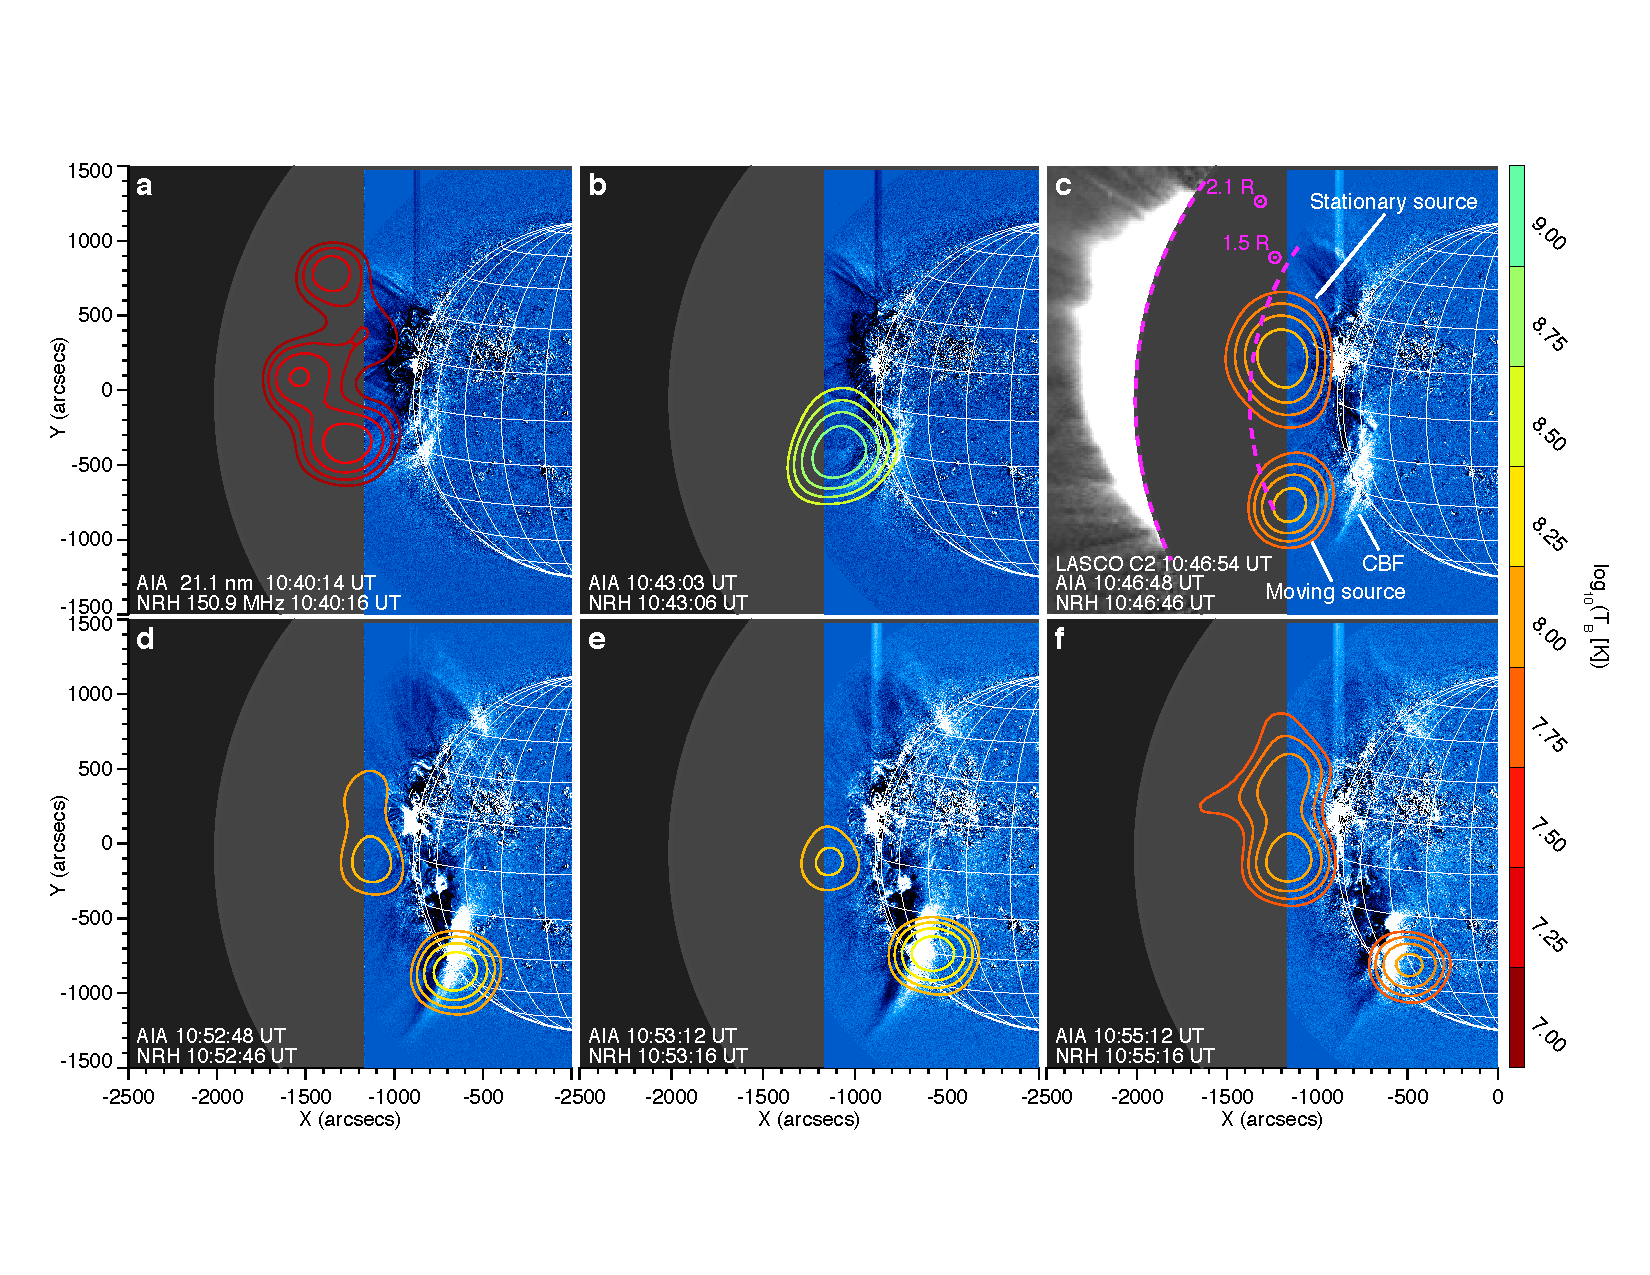
\includegraphics[scale=0.7, trim=0cm 2.5cm 0cm 1.5cm]{gallagher_figure1_final.pdf}
	\caption[Propagation of CBF and radio burst]{{\bf a-f} show that the 150\,MHz source follows closely the coronal bright front (CBF) as it propagates around the east limb, indicating they belong to a common structure. The intensity of the radio source is indicated by the colour bar on the right. {\bf c} reveals the role of the CME in the event, as observed by the LASCO C2 coronagraph. The combination of the white-light coronagraph (C2) and the EUV images (AIA) reveal the full spatial extent of the CME bubble i.e., the frontal structure in white-light has clear extensions back toward the solar surface, imaged at EUV. The location of the radio source and CBF show they clearly have a relationship with the southward CME flank.}
	\label{fig:figure_aia_nrh_c2}
\end{sidewaysfigure}
%
%
In each image the contours range from $T_{peak}$ to $0.95T_{peak}$, where $T_{peak}$ is the peak brightness temperature at the time of the image; the intensity of the contours is indicated by the colour bar on the right. Initially, both the erupting structure seen in the AIA image and the radio source had the same spatial extent over latitude (Figure.~\ref{fig:figure_aia_nrh_c2}a), showing they belong to a common structure. After this, the most southern part of the radio source reached an extremely high brightness temperature ($\sim$10$^9$\,K) and closely followed the propagation of the CBF southward until it eventually diminished into the thermal background at 10:56\,UT. Another emission source at 150.9\,MHz was also observed at $\sim$$0^{\circ}$ latitude on the east limb at a height of 1.1--1.3$\,R_{\odot}$ (Figure.~\ref{fig:figure_aia_nrh_c2}c,d,e,f); while this source was clearly associated with the eruptive active region, any link between it and the CBF is secondary, as it shows no temporal relationship with the start and stop time of the bright front. Similar radio source motion is observed at 173, 228 and 270\,MHz, however any co-propagation of these radio sources with the CBF is of much shorter duration. Figure.~\ref{fig:figure_aia_nrh_c2}c 
reveals the role of the CME in the event, as observed by the LASCO C2 coronagraph. The combination of the white-light coronagraph (C2) and the EUV images (AIA) reveal the full spatial extent of the CME bubble i.e., the frontal structure in white-light has clear extensions back toward the solar surface, imaged at EUV. The location of the radio source and CBF show they clearly have a relationship with the southward CME flank.

%A movie showing the co-propagation of the CBF and 150\,MHz radio source can be found in Supplementary Movie 1. For a movie and discussion of the multi-thermal nature of the CBF see Supplementary Movie 2.


%-------------- Data Analysis -----------------------%
\subsection{Radio Source Height and Speed}
To compare the motion of the CBF and radio source, the position angle (PA) trajectories were analyzed (Figure.~\ref{fig:angle_time}). Here position angle is measured in degrees counter-clockwise from solar north. The solid lines show a fit of $\theta(t) = \theta_0 + \omega t$ to the data, where $\theta_0$ is the starting PA, $\omega$ is the angular velocity, and $t$ is time. The slope of each line gives $\omega$, from which the velocity of the source may be obtained using $v=r\omega$, where $r$ is the distance of the source from Sun center. 
\begin{figure}[!t]
\begin{center}
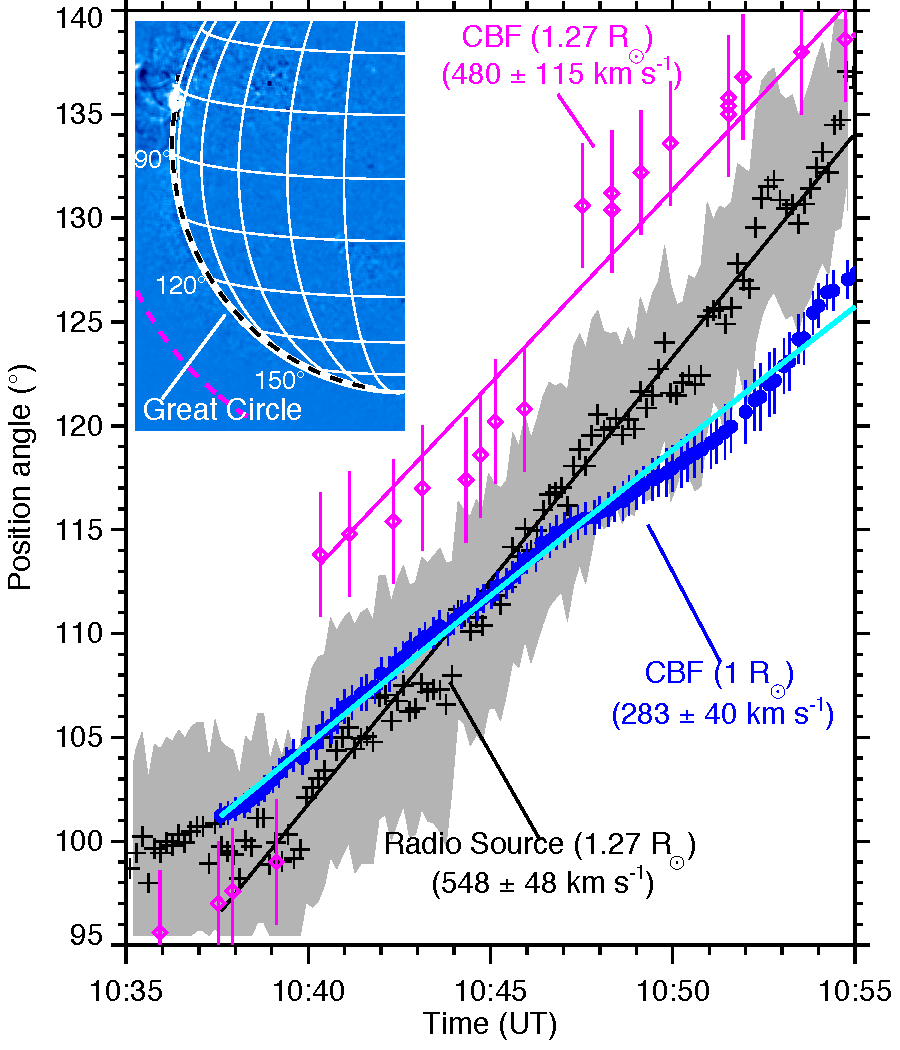
\includegraphics[scale=0.7, trim=1cm 0cm 0cm 0cm]{gallagher_figure2_final.pdf}
\caption[Radio source and CBF position angle versus time]{Position angle (degrees anticlockwise from solar north) versus time for the 150\,MHz source, shown in plus signs, and coronal bright front (CBF) at $1\,R_{\odot}$ (circles) and $1.27\,R_{\odot}$ (diamonds). The great circle along which the CBF was tracked at $1\,R_{\odot}$ is indicated by the dashed white line in the inset; the dashed pink line marks a height of $1.27\,R_{\odot}$. Both radio burst and CBF have a consistent propagation in the same direction and have similar speeds at a height of $1.27\,R_{\odot}$, implying they belong to a common propagating coronal structure. The uncertainty on radio source position angle is taken to be from 1$\sigma$ uncertainties of the source width ($\sim$7$^{\circ}$) plus the fluctuation of source position due to coronal and ionospheric scattering effects ($3^{\circ}$ at frequencies up to 160\,MHz \citep{stewart1982}). The CBF position uncertainty is from Gaussian centroid uncertainty from a tracking and fitting algorithm of the CBF pulse \citep{long2011a}.}
\label{fig:angle_time}
\end{center}
\end{figure}

%----------------- Height of radio source ----------------------%
The 150\,MHz source had an angular velocity of $6.2\pm0.1\times10^{-4}\,\mathrm{rad\,s^{-1}} $. In order to estimate the height of the radio source we first convert from frequency to electron number density using equation~\ref{eqn:plasma_frequency}. Usually, there would be a conversion of this plasma frequency using the density models described in Section~\ref{sec:freq_drift}. However, as outlined, these models can often provide a poor description of the corona and lead to an evaluation of height for the radio burst that may be incorrect. For a more reliable calculation of radio source height we derive density models from data, rather than relying on a `guess' model.

%Given the radio source had a frequency of emission of 150\,MHz, we first convert to density using equation (3) below, and assuming that the emission is harmonic, this results in a density of $n_e=6.9\times10^7$\,cm$^{-3}$. 
Both the LASCO C2 coronagraph and AIA were used for density diagnostics of the corona. Firstly, six AIA passbands were used to create emission measure and density maps of the corona from 1.0--1.3\,$R_{\odot}$ (Zucca et al. 2013), following the method outlined in \citep{asch2013}, details are provided in Appendix~\ref{app:densities}. From 2.0--4.0\,$R_{\odot}$ density diagnostics were performed using the LASCO C2 coronagraph \citep{vdeh50}. Density diagnostics via white-light studies involve the Thomson scattering theory and van de Hulst coefficients, also described in Appendix~\ref{app:densities}. The density diagnostics of AIA and LASCO C2 are combined into a single density image. This results in density values from 1.0--4.0\,$R_{\odot}$, but with a gap in measurement between the two fields of view of the two telescopes (1.3--2.5\,$R_{\odot}$). In order to fill this gap a hybrid of a plane parallel and a spherically symmetric hydrostatic equilibrium (HE) model were fit to the density data from AIA and C2 to form a continuous density map from 1.0--4.0\,$R_{\odot}$. This hybrid model model has the form
\begin{equation}
%n(r) = n_{ar}\mathrm{exp}\bigg(-\frac{\mu m_pgr}{kT}\bigg) + n_{qs}\mathrm{exp}\bigg[\frac{\mu m_pGM_{\odot}}{kTR_{\odot}} \bigg(\frac{R_{\odot}}{r}-1\bigg)\bigg]
n(r) = n_{ar}\mathrm{exp}\bigg(-\frac{r}{H}\bigg) + n_{qs}\mathrm{exp}\bigg[-\frac{1}{H} \bigg(\frac{1}{R_{\odot}}-\frac{1}{r}\bigg)\bigg]
\label{eqn:hybrid_hydro}
\end{equation}
where $r$ is heliocentric distance and $H=kT/\mu m_pg_{\odot}$ is the scale height, where $T$ is temperature, $k$ is Boltzman's constant, $m_p$ is a proton mass, $\mu$ is mean molecular weight, and $g_{\odot}$ is acceleration due to gravity at $1\,R_{\odot}$. Here, the plane parallel model for $n_{ar}$ corresponds to the active region of the data derived from the EUV images, while the spherically symmetric model corresponds to the quiet corona ($n_{qs}$) C2 data. A spherical symmetric model is used for the coronagraph data because the range in heights given by the C2 data will be associated with decreasing gravity (as opposed to the constant gravity over the active region height range). This density model is fit for every position angle such that a 2D map of electron density values in the corona may be obtained (Figure~\ref{fig:density_map}).
\begin{figure}[t!]
\begin{center}
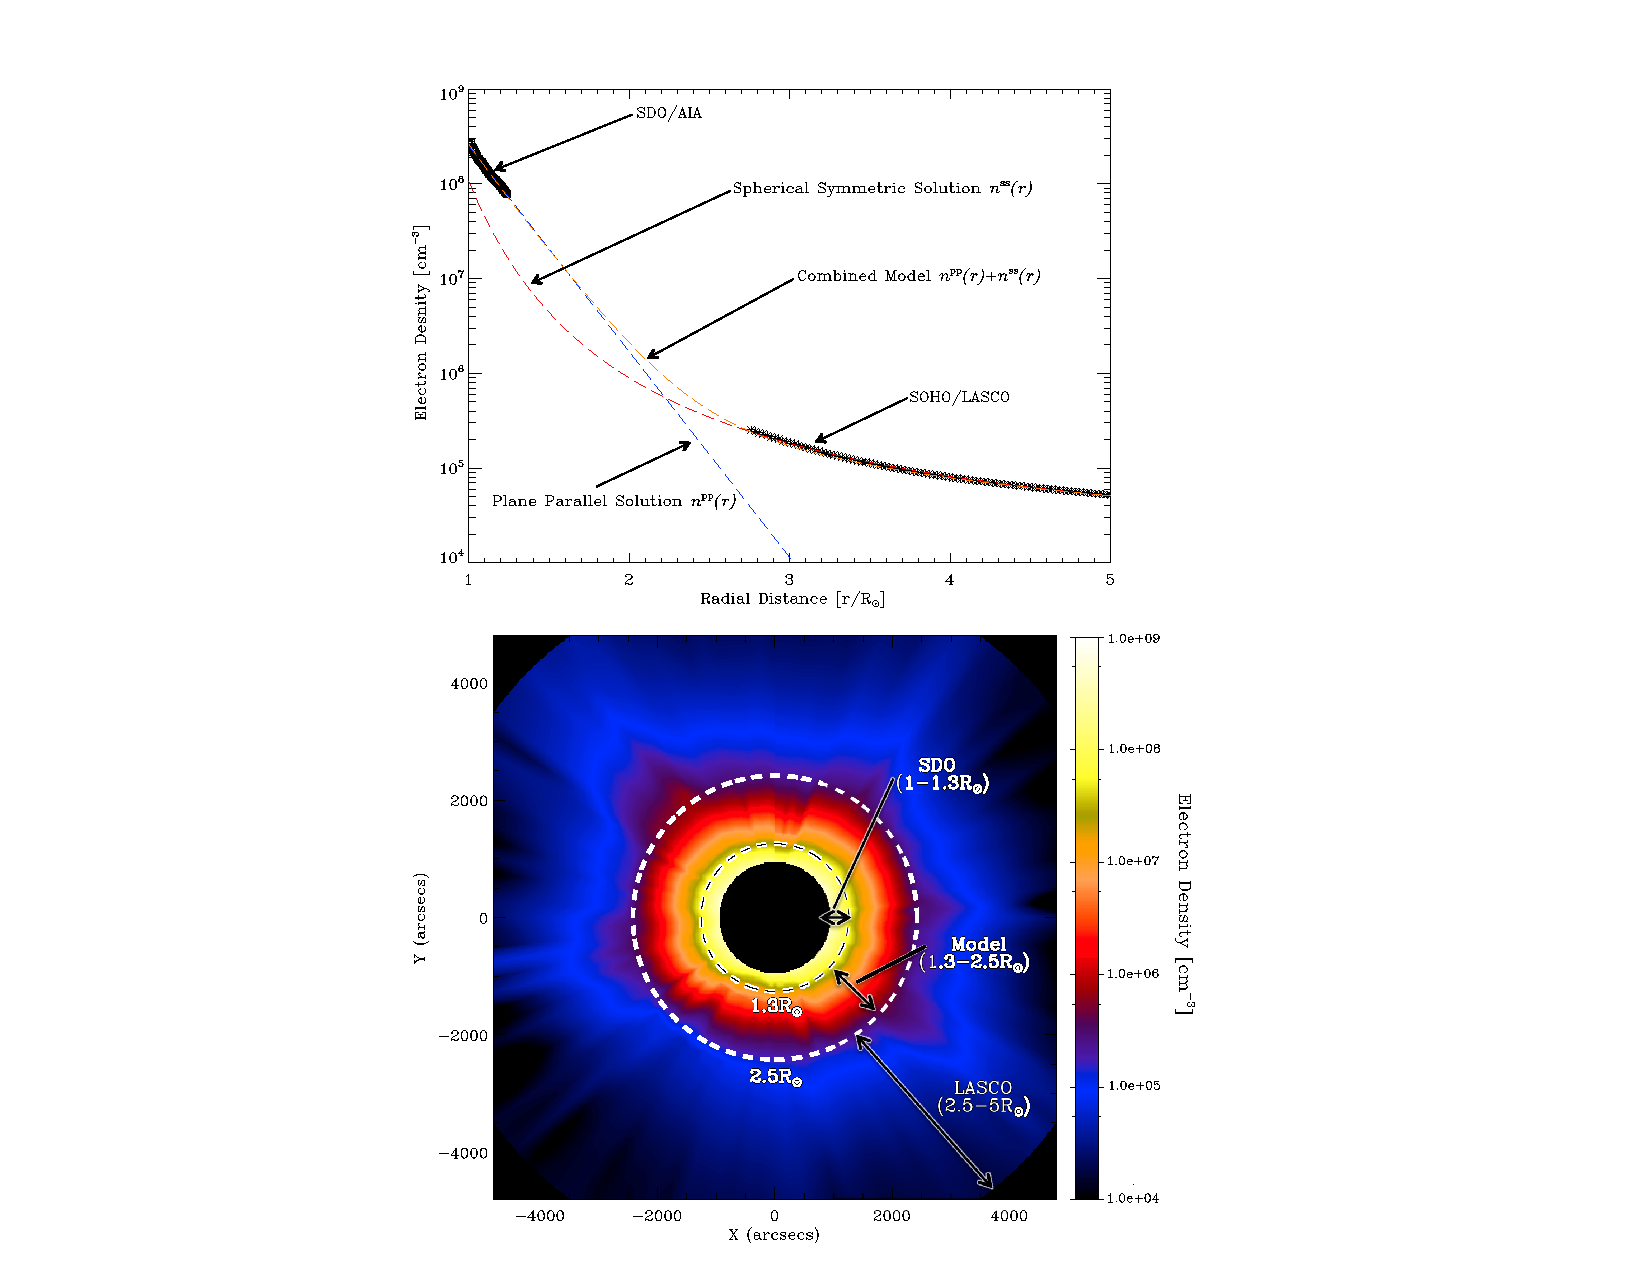
\includegraphics[scale=0.8, trim=4cm 0cm 0cm 1cm]{pietro_density.pdf}
\caption[2D density map of the corona]{(Top) A single radial trace showing the density data derived from AIA and C2. The plane parallel model (blue dash), spherically symmetric model (red dash), and hybrid model (orange dash) are indicated. Mean molecular weight of 0.6 and temperature of $1.4\times10^{6}$\,K were used in Equation~\ref{eqn:hybrid_hydro} (Bottom) A 2D density map created from the hybrid model applied to density data at all position angles 
Density maps such as this can provide much better estimates of radio source height, rather than using a density model which may provide a poor description of the corona.}
\label{fig:density_map}
\end{center}
\end{figure}

These density diagnostics allowed a determination of the height from which 75\,MHz originated (assuming that 150\,MHz observations are of harmonic plasma emission). We find that over the range of the position angles encountered by the radio source (100-140$^{\circ}$), this frequency occurs at an average height of $1.27\,R_{\odot}$, with a maximum height of $1.31\,R_{\odot}$ and a minimum height of $1.21\,R_{\odot}$. We must also take into account that the density measurements themselves have an uncertainty. To account for this, we add the measurement uncertainty (15\%) to the density values and determine the maximum possible height of 75\,MHz in the position angle range, then we subtract 15\% from the density values and measure the minimum possible height. This results in a heliocentric distance of $1.27^{+0.06}_{-0.09}\,R_{\odot}$ for the radio source. This position, including uncertainties, combined with the value for angular velocity ($6.2\pm0.1\times10^{-4}\,\mathrm{rad\,s^{-1}} $) gives the tangential velocity of $548^{+34}_{-48}$\,km\,s$^{-1}$ for the radio source.


\subsection{Radio Source Alfv\'{e}n Mach}

To determine whether or not the radio source motion super-Alfv\'{e}nic, the Alfv\'{e}n speed of the environment through which it propagated was estimated. An estimate of the Alfv\'{e}n speed requires a measure of density (which was derived above) and magnetic field using 
\begin{equation}
v_A = \frac{B}{\sqrt{4\pi n_p \mu m_p}}
\end{equation}
where $B$, $\mu$ is the mean molecular weight taken to be 0.6 for the corona, $n_p$ is the proton number density (same as electron number density for fully ionized hydrogen plasma), and $m_p$ is proton mass. To estimate the magnetic field strength, we used a potential field source surface (PFSS) extrapolation of the coronal magnetic field on the 22-Septemper-2011 06:04\,UT, shown in Figure~\ref{fig:pfss}. 
This was performed using the SolarSoft package of \citet{schrijver2003} and data from the Helioseismic and Magnetic Imager (HMI)\citep{scherrer2012} of the SDO spacecraft. Green and pink lines signify open field regions while white is closed field.
\begin{figure}[t!]
\begin{center}
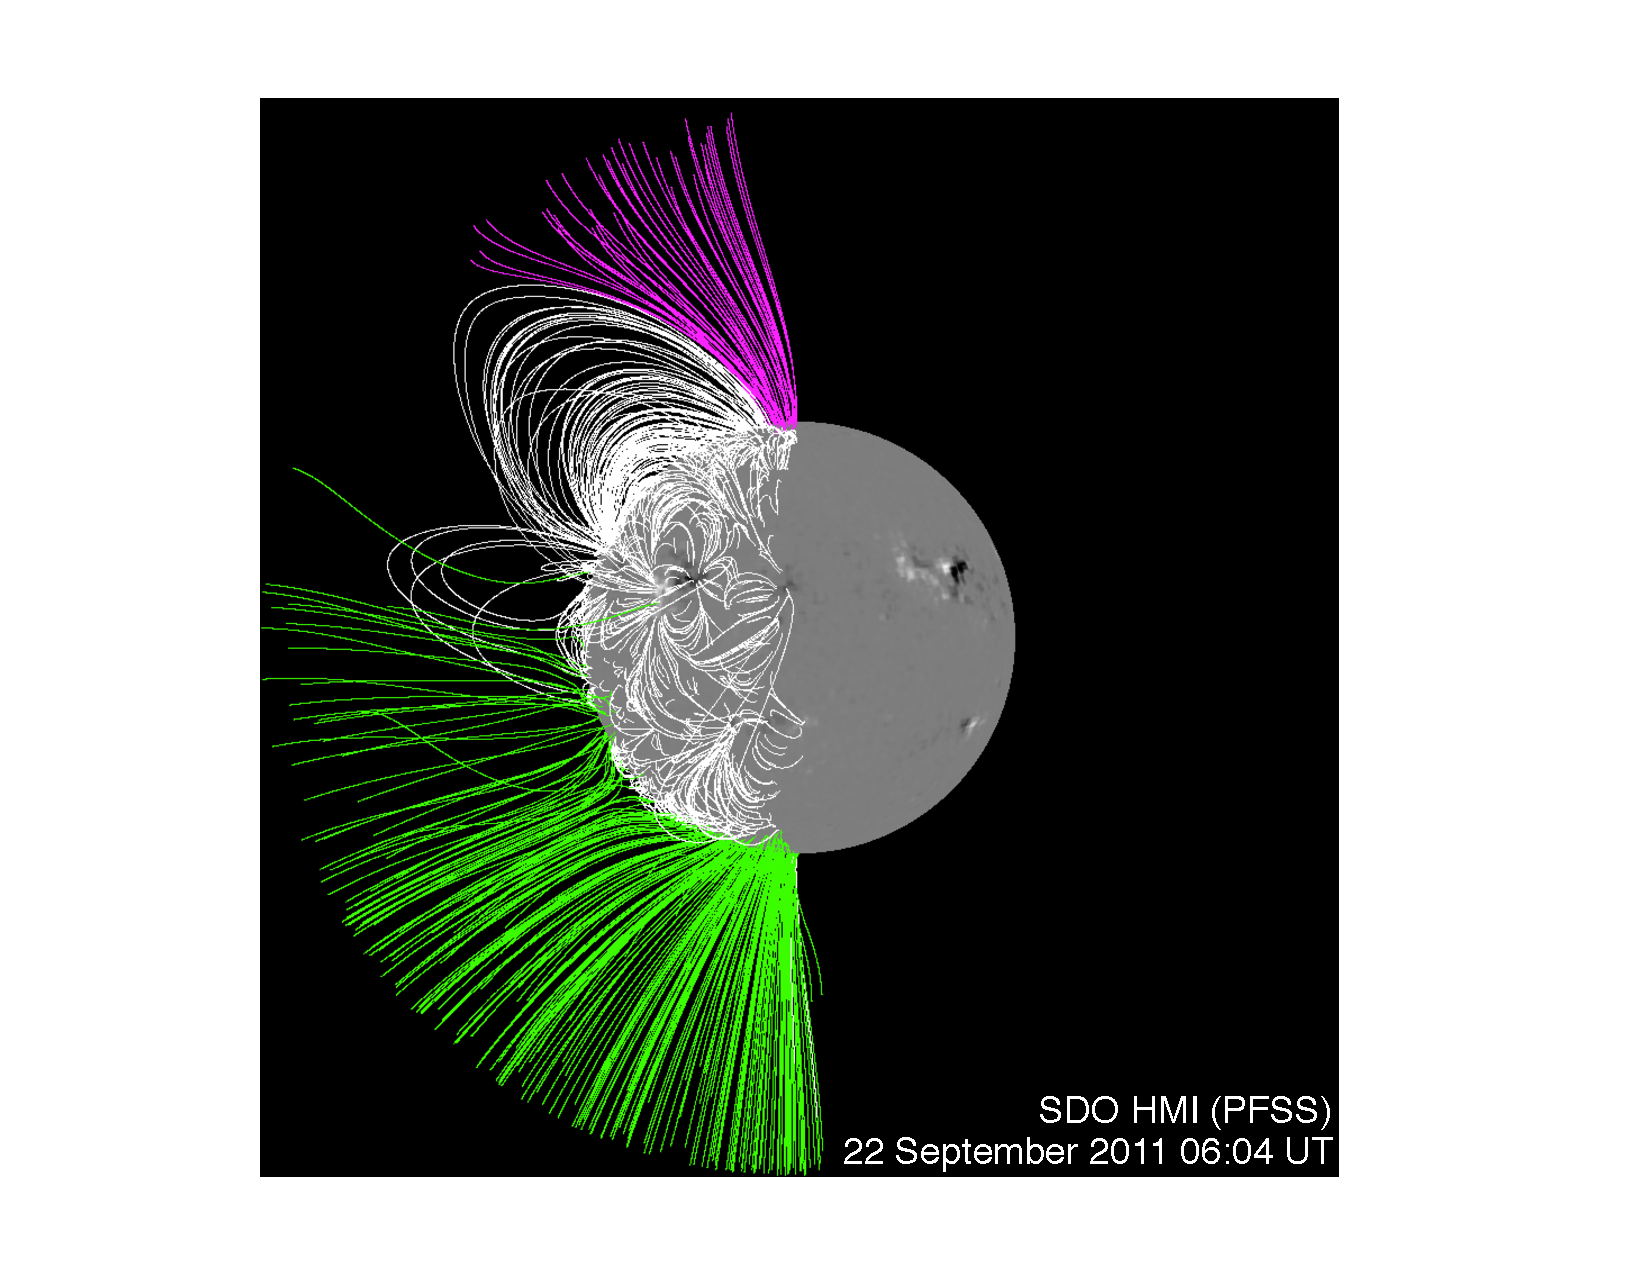
\includegraphics[scale=0.6, trim=1cm 1cm 0cm 1cm]{gallagher_supplem_fig2_final.pdf}
\caption[A potential field source surface extrapolation of the corona magnetic field]{A potential field source surface (PFSS) extrapolation of the coronal magnetic field on the 22-Septemper-2011 06:04\,UT. This was performed using the SolarSoft package of \citet{schrijver2003} and data from the Helioseismic and Magnetic Imager (HMI)\citep{scherrer2012} of the SDO spacecraft. Green and pink lines signify open field regions while white is closed field. The CBF and CME flank propagated through the south-east quadrant. Therefore a transverse propagation through these open and closed field structures suggests that the shock was likely of quasi-perpendicular orientation.}
\label{fig:pfss}
\end{center}
\end{figure}
The PFSS extrapolation provides magnetic field was combined with the density map to produce a 2D Alfv\'{e}n speed map of the corona, such that the Alfv\'{e}n speed position may be obtained for any position in the 2D sky-plane. This is the first time such empirical values of density and magnetic field have been produced for the 2D sky-plane. 
At the source heliocentric distance of $1.27\,R_{\odot}$ we find $B=0.67$\,G. Combining this with the density at the radio source results in an Alfv\'{e}n speed of $225$\,km\,s$^{-1}$. 
%
%
%
\begin{figure}[t!]
\begin{center}
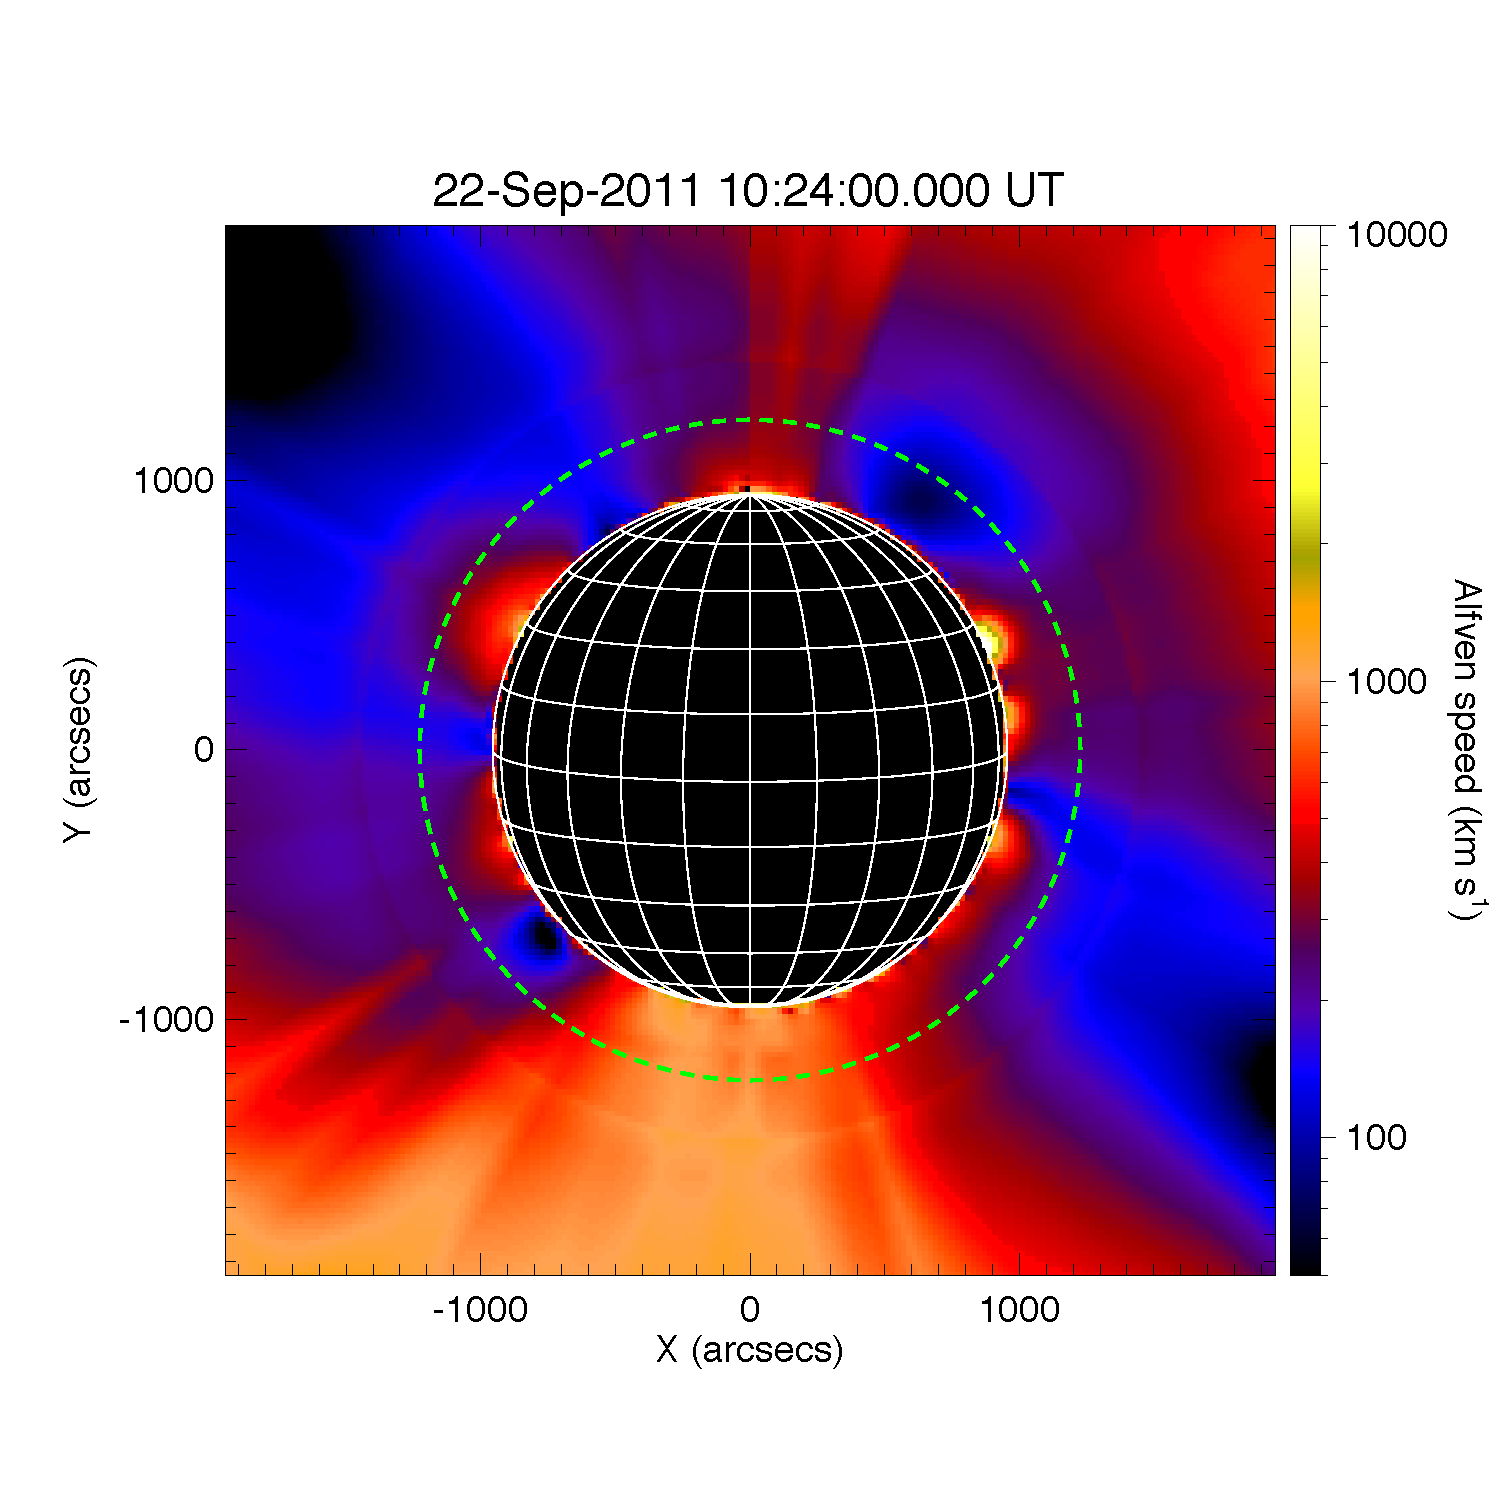
\includegraphics[scale=0.5, trim=1cm 2cm 0cm 3cm]{thesis_alfven_map.pdf}
\caption[Alfv\'{e}n speed map of the solar corona.]{Alfv\'{e}n speed map of the solar corona, derived from density values using LASCO C2, SDO/AIA, and magnetic field values from the PFSS extrapolation. These empirical observations have features which were predicted by the model Alfv\'{e}n produced by \citet{warmuth2005} i.e., the presence of minima in Alfv\'{e}n speed close to active regions. The greed circle marks a height of 1.27\,$R_{\odot}$. Figure adapted from Zucca \& Carley\,{\it et.\,al.} (submitted)}
\label{fig:pfss}
\end{center}
\end{figure}
%
%
%
Taking into account that the source may be in the range from $1.18-1.33\,R_{\odot}$, we find a possible range of $0.5-0.9$\,G for the magnetic field that the source may encounter between the position angles of $100-135^{\circ}$. Again using the density at the radio source we find the possible range in Alfv\'{e}n speeds that the source may encounter is $190-310$\,km\,s$^{-1}$. Hence we quote the Alfv\'{e}n speed as $v_A=225^{+85}_{-35}$\,km\,s$^{-1}$. Using the speed of the source we then find the Alfv\'{e}n Mach to be $M_A =2.4^{+0.7}_{-0.8}$. We note that it is not possible to estimate an error on the magnetic field strength since it is an extrapolation from the surface field, however, the results of super-Alfv\'{e}nic Mach are tolerant to within 50\% uncertainty on the PFSS B-field estimate. Also, the PFSS represents the lowest energy state of the coronal magnetic field, hence this Mach number is taken to be an upper limit.

Finally, the direction of the field is also given by the PFSS extrapolation. It shows an extended region of open and radial field structure in the south east quadrant of the corona, with a weak closed field region on disk in this quadrant. The shock propagated transversely through this region, showing there is a strong possibility of the shock encountering quasi-perpendicular orientation of the magnetic field. As was described in Section~\ref{sec:sda_discussion}, quasi-perpendicular orientation is an essential aspect of the SDA process and generation of plasma emission


\subsection{CBF Speeds}
In a similar approach to the radio source motion, the CBF motion was tracked along a great circle at the solar limb to obtain its position angle trajectories with time Figure~\ref{fig:angle_time}. These positions are shown as blue circles in Figure~\ref{fig:angle_time}. The solid blue line shows a fit of $\theta(t) = \theta_0 + \omega t$ to the data, where $\theta_0$ is the starting PA, $\omega$ is the angular velocity, and $t$ is time. Again, the slope of each line gives $\omega$, from which the velocity of the source may be obtained using $v=r\omega$, where $r$ is the distance of the source from Sun center. 
For the CBF, an angular velocity of $4.1\pm0.4\times10^{-4}$\,rad\,s$^{-1}$ was obtained, resulting in a velocity of $283\pm40$\,km\,s$^{-1}$ at $1\,R_{\odot}$. Although the radio source and CBF show a consistent propagation southwards, the CBF does so at a slower speed, possibly because it is at a smaller height than the radio source. To compare the motion of the CBF and radio source at the same height, the CBF motion was tracked at $1.27\,R_{\odot}$. The CBF was much fainter and more diffuse at this height, hence their are fewer data points and the errors are larger than the $1\,R_{\odot}$ data. At $1.27\,R_{\odot}$, the CBF was found to have an angular velocity of $5.4\pm1.3\times10^{-1}$\,rad\,s$^{-1}$, resulting in $v=480\pm115$\,km\,s$^{-1}$. Both the CBF and radio source clearly show common kinematics at a similar height of $1.27\,R_{\odot}$, with the two features having a consistent progression southward around the east limb. 

\subsection{CBF Thermal Properties}
\begin{figure}[t!]
\begin{center}
\includegraphics[scale=0.52, trim=0cm 10cm 0cm 2cm]{tri_color.pdf}
\caption[Tri-color running ratio images of a CBF.]{Tri-colour running ratio images of the 22-September 2011 CBF, produced from 171, 195 and 211\,\AA~images from SDO. These images are used to discern an general temperature changes of the front as it propagates, with blue color regions indicating a relative cooling, and red/yellow regions indicating a relative heating.}
\label{fig:tri_color}
\end{center}
\end{figure}
In order to investigate any thermal properties of the CBF we have produced tri-colour running ratio images of the CBF, shown in Figure~\ref{fig:tri_color}. A ratio image is one in which the image of interest is divided by a pre-event image e.g., the one direct preceding the image of interest. Any intensity increase will show up as a brightness enhancement. A tri-colour running ratio image is one where three separate filters are used to represent running a running ratio in the the three channels of a Red-Green-Blue (RGB) image. The assignment of the RGB color channels are 171 (blue), 193 (green), and 211� (red). As described in detail in \citet{downs2012}: {\it ``a particular offset in the relative phases or amplitudes of the perturbation for each channel will be spread across the RGB color plane. By nature this representation highlights anticorrelated ratio phases as having strong color components. Correlated phases on the other hand will be confined to a mostly gray-scale range."} 

Since each filter used in the images is sensitive to different temperature ranges a tri-colour movie may indicate a local temperature change due to a passing transient. For example, a positive temperature perturbation (heating) may show up as excess emission in 19.3\,nm and/or 21.1\,nm passbands resulting in a orange/yellow appearance. A negative temperature perturbation (cooling) will result in excess 17.1\,nm channel (6.3$\times$10$^5$\,K) combined with a deficiency in 19.3\,nm (1.2$\times$10$^6$--2$\times$10$^7$\,K) and 21.1\,nm ($\times$10$^6$\,K) channels; this results in a blue appearance in the image. In this way, we can qualitatively identify what parts of the CBF are due to local heating and what parts are due to cooling \citep{cohen2009, downs2012, cheng2012}. The furthermost front has a yellow appearance, indicative of a positive temperature perturbation, with a secondary blue (cooler) front behind it. This is the expected behaviour of a propagating pressure pulse i.e., a traveling pressure perturbation will result in a slight heating followed by a rarefaction and cooling in its wake \citet{downs2012}. This is further confirmation that the CBF observed in this event is indeed a pressure pulse, making it more likely to be associated with shock activity higher in the corona.

\section{Radio Dynamic Spectra}\label{sec:20}

While the NRH imaging data reveal there was a high intensity radio source closely associated with the CBF, the radio dynamic spectroscopy reveal exactly what kind of radio activity this is. Section~\ref{sec:freq_drift} shows that different types of physical activity in the corona, such as particle acceleration and shock activity can be recognised by their characteristic signature in dynamic spectra. 

\subsection{Observations}
The 150\,MHz source observed by NRH had a brightness temperature of $\sim$$10^9$\,K, indicating coherent plasma emission. As decribed in Sections~\ref{sec:wave_particle}--\ref{sec:three_wave}, plasma emission is generated via plasma oscillations that are due to instabilities in the presence of high velocity electron beams. The presence of electron beams was independently verified and revealed in detail using radio dynamic spectra. At $\sim$10:40\,UT the fundamental and harmonic bands of a type II burst shock signature was observed at 45 and 90\,MHz (Figure~\ref{fig:dyn_spec}b), respectively, using the Nan\c{c}ay Decametric Array \citep[NDA;][]{boischot1980}. Type III bursts begin at the same time as the type II (Figure~\ref{fig:dyn_spec}a,b), observed using NASA's STEREO-B/WAVES instrument \citep{bougeret2008}. The speeds of these particles could be obtained from their frequency drift.

\subsection{Particle speeds and in-situ detection}
The frequency drift of these type III radio bursts provide a measure of velocity of the electrons causing the radio emission by converting frequency-time measurements to height-time via a coronal density model. From the dynamic spectra, it is possible to obtain a set of frequency time measurements $(f_i,t_i)$, in this case along the left edge of the type III. Using the expression for plasma oscillation (Equation~\ref{eqn:plasma_frequency}), the set $(f_i,t_i)$ may be converted into a set of density time values $(n_i,t_i)$. In order to convert these into a height-time set $(r_i,t_i)$, a density model of the solar corona is used. The density model in this case is derived from a solution to the Parker solar wind equation which is used specifically to analyze low frequency (interplanetary) type IIIs \citep{Mann1999}. Once this $(r_i,t_i)$ height-time set was found, we took into account that the electron beams are traveling along open magnetic field lines which follow the Parker spiral. In cylindrical coordinates, the radius $r$ and azimuthal angle $\phi$ share the relationship $r-r_0= -\frac{v_{sw}}{\Omega_{\odot}}( \phi - \phi_0)$ i.e., an Archimedean spiral with parameters $v_{sw}$, the solar wind velocity, and $\Omega_{\odot}$, the angular velocity at solar equator. The arch-length along any arm of this spiral (along an open magnetic field line) is given by
\begin{equation}
s(\phi) = \frac{v_{sw}} {2\Omega_{\odot}}\big(\phi\sqrt{1+\phi^2} + \mathrm{arcsinh}(\phi)  \big)
\end{equation}
where arcsinh is the inverse hyperbolic sine function. Using a solar wind velocity value of 450\,km\,s$^{-1}$ (observed in-situ using the STEREO-B PLASTIC)
\begin{sidewaysfigure}[!t]
    \centering
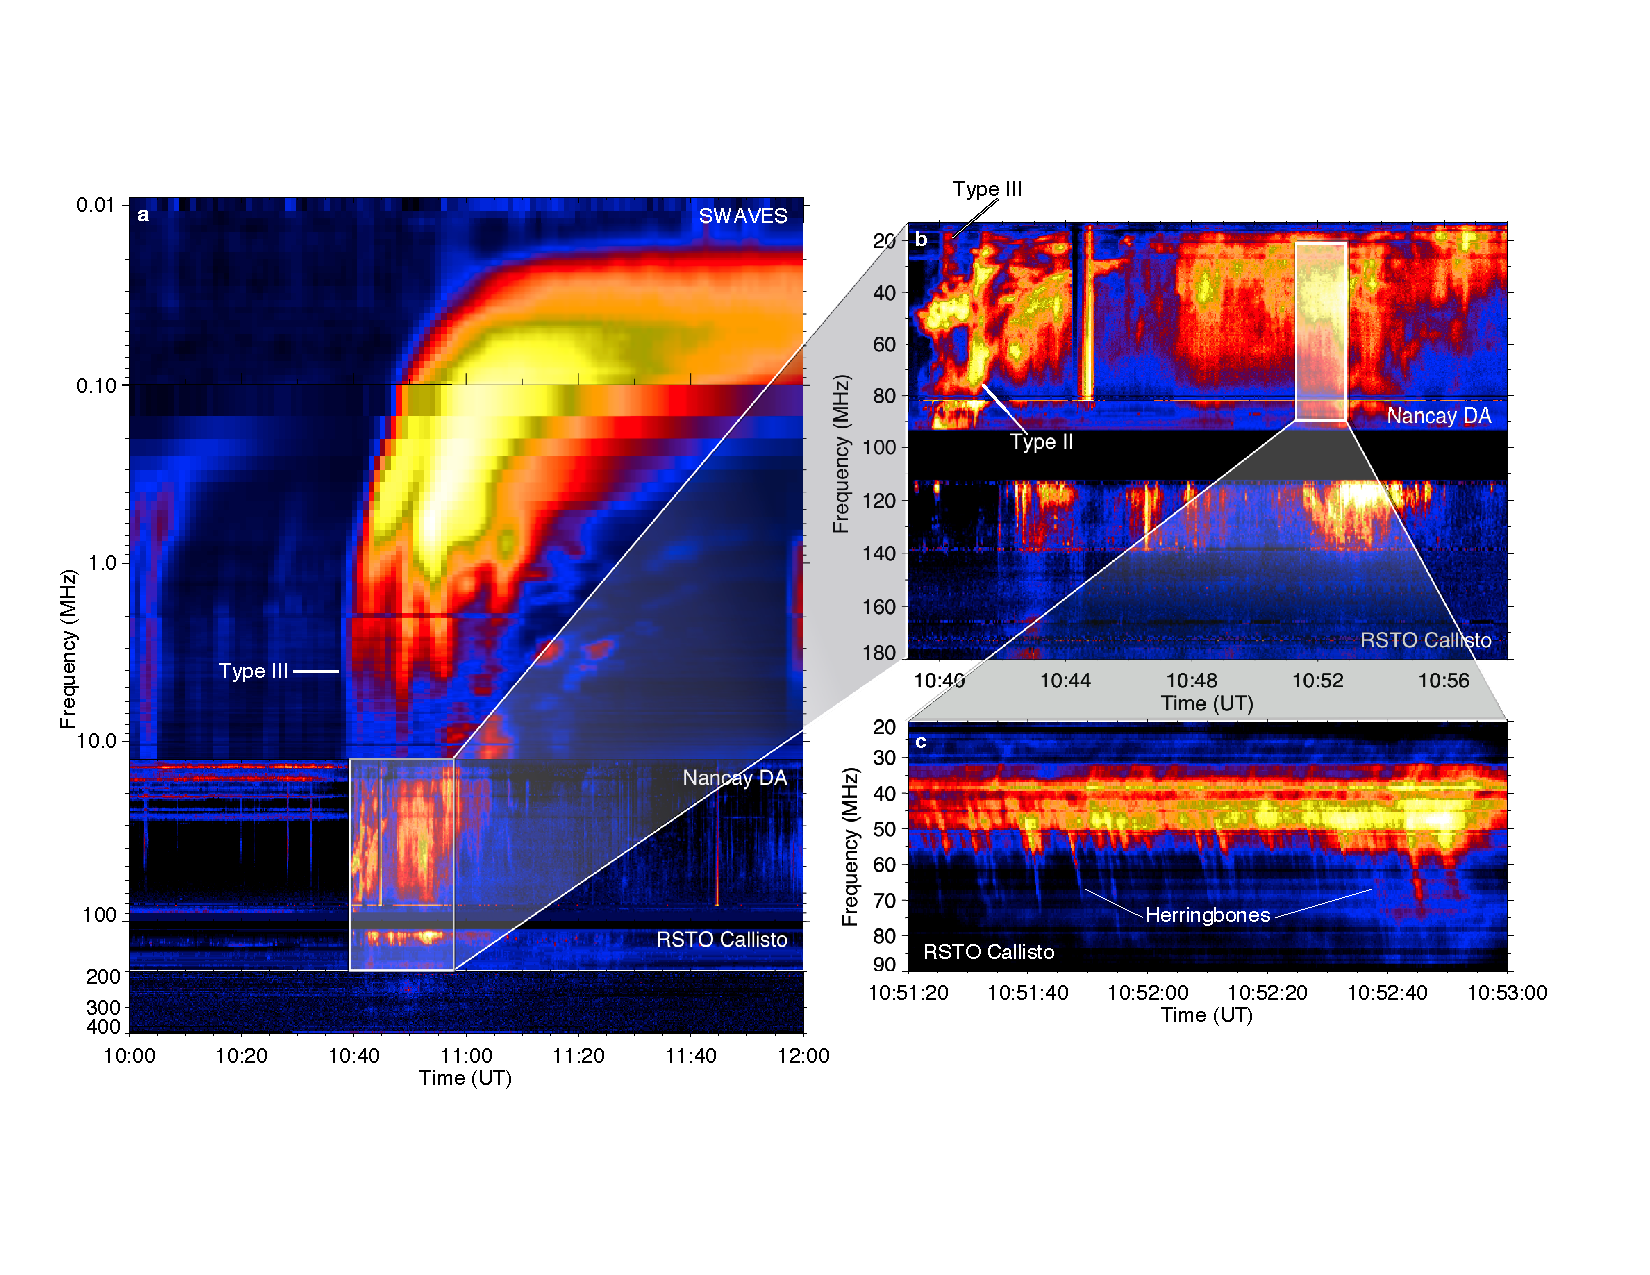
\includegraphics[scale=0.7, trim=0cm 3cm 1cm 4cm]{gallagher_figure3_final.pdf}
\caption[Radio dynamic spectra of 22-September-2011 event]{Radio dynamic spectra from STEREO-B/WAVES (0.01--16\,MHz), Nan\c{c}ay DA (20--90\,MHz), and RSTO eCallisto (10--400\,MHz). The type II radio burst is indicated in {\bf b}, with both fundamental and harmonic emission observable. This shock signature is characterized by two emission bands drifting slowly ($\sim$-0.2\,MHz\,s$^{-1}$) toward lower frequency over time. The type III bursts are indicated in {\bf a},{\bf b}, while herringbones are shown in {\bf c}. Each herringbone or is indicative of an electron beam traveling away from the shock. Note that all of the radio activity from {\bf a-c} is indicative of either particle acceleration or a plasma shock in the corona. The start and stop times of this radio activity in these dynamic spectra show good temporal correspondence with the start/stop times of the activity in Figure~\ref{fig:figure_aia_nrh_c2}. This is especially apparent for the features between 100--200\,MHz.}
\label{fig:dyn_spec}
\end{sidewaysfigure}
\clearpage
\noindent
and $\phi=\frac{ \Omega_{\odot}}{v_{sw}}r=-6.5\times10^{-12}$\,rad\,m$^{-1}\times r$, the set $(r_i,t_i)$ were converted to a set of distances along the Parker spiral vs time $(s_i, t_i)$. A linear fit to this data then gives the speed of electrons producing the type III as 0.4\,$c$ (Figure~\ref{fig:typeIII_speeds}). Note that since the $(f_i, t_i)$ points are taken along the left edge of the type III burst, this speed is representative of the fastest electrons contributing to the radio burst. 

It is difficult to estimate an error on this speed, due to a lack of interplanetary density measurements from which this speed is derived, we may confirm the presence of particles with such energy from in-situ data. Figure~\ref{fig:sept} shows a plot of electron flux versus time from the Solar Electron Proton Telescope (SEPT)\citep{muller2008} onboard STEREO-B. It shows an increase in electron flux in the range of 45 - 325\,keV. The vertical black line is the expected time of arrival of the electrons causing the type III burst, calculated from their speed and distance travelled on the Parker spiral. The expected time of arrival of the type III electrons match quite well the first peak in flux of the in-situ detected electrons, showing that the speeds derived from frequency drift are a reliable estimate.

\begin{figure}[!t]
\begin{center}
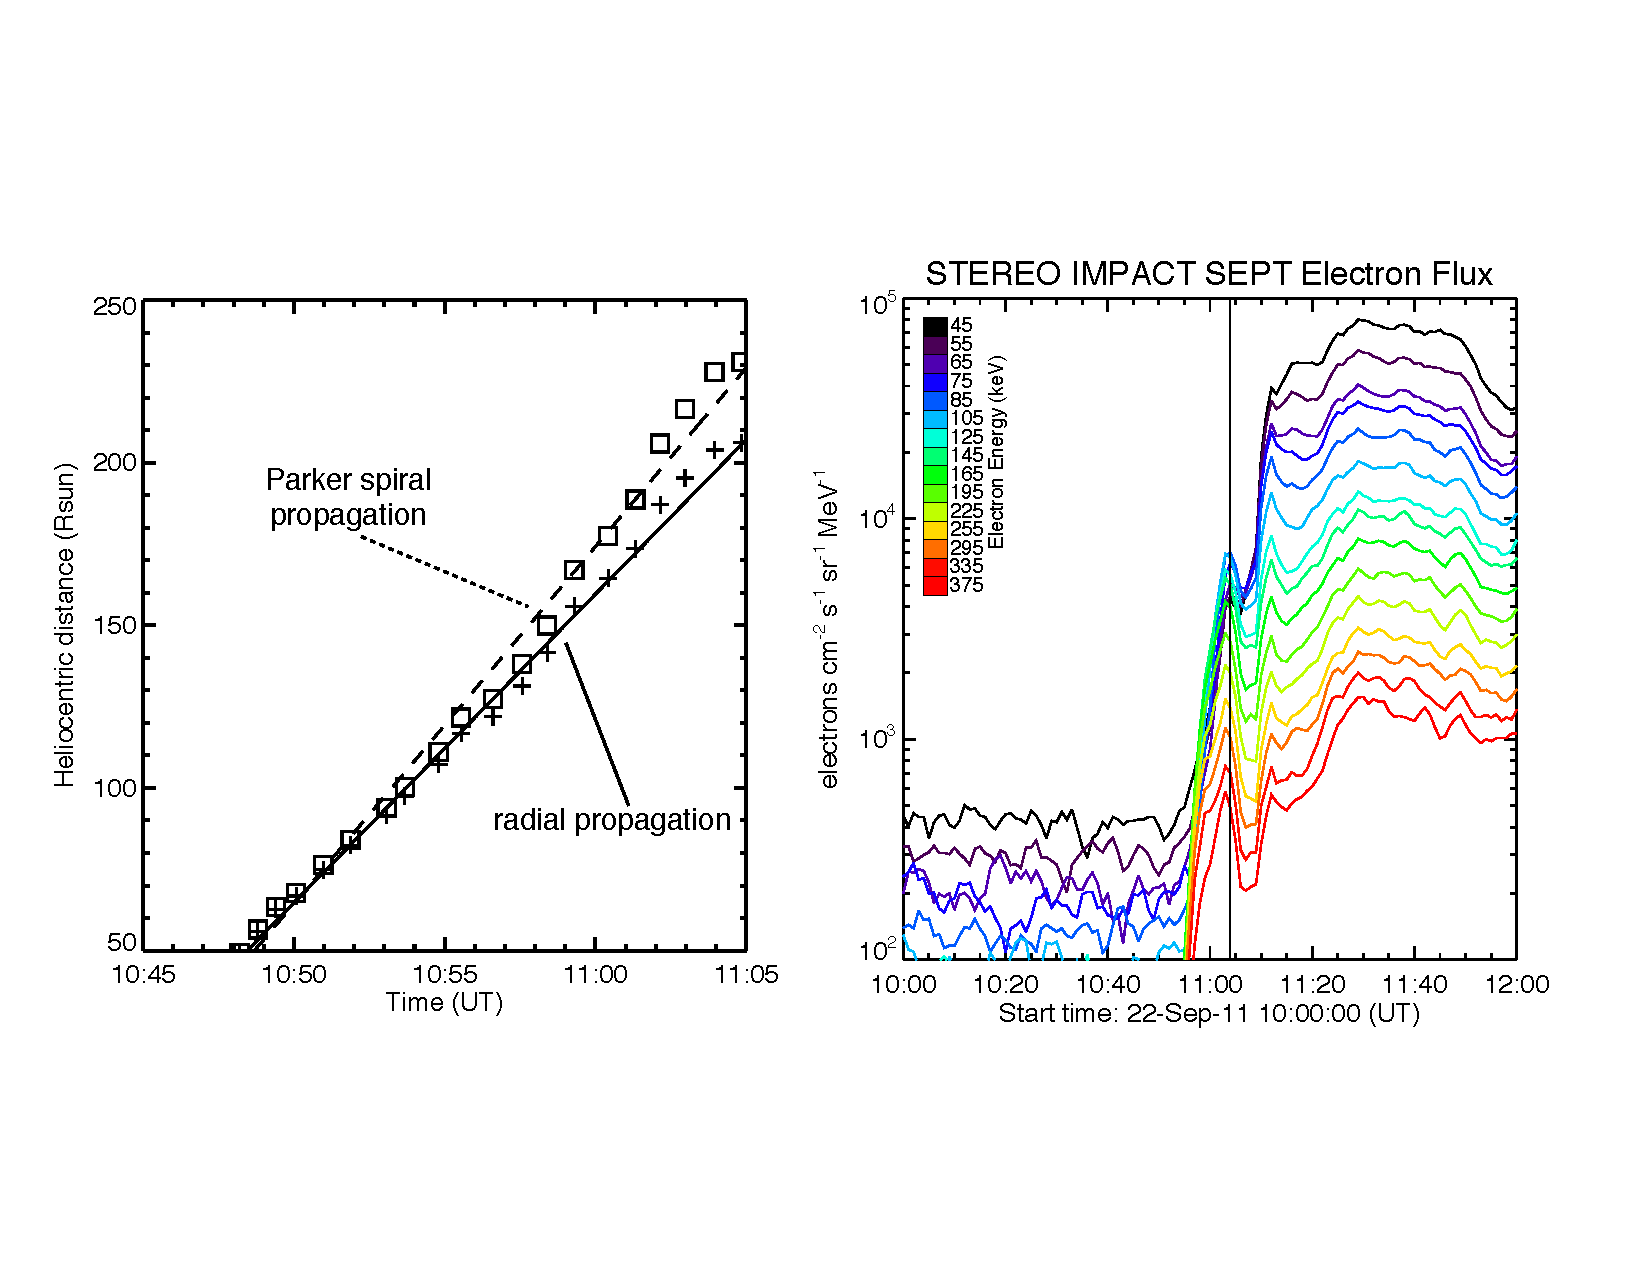
\includegraphics[scale=0.6, trim=1.7cm 4cm 0cm 5cm]{typeIII_speeds.pdf}
\caption[Type III speeds]{(Left) Distance-time for points chosen along the right edge of the type III radio burst observed by S/WAVES. Both radial and Parker-spiral corrected points are shown. (Right) Detection of electrons in-situ by SEPT on STEREO-B. The electrons arrive at $\sim$11:05\,UT, approximately 35 minutes after the flare start time. The black vertical line indicates the expected time of arrival (ETA) of the type III electrons. This ETA was calculated from the electron speed (derived from the frequency drift and a density model), and the distance travelled along the Parker spiral (given a solar wind speed of 450\,km\,s$^{-1}$). Note that the type III electrons, calculated to have an energy of 46\,keV, have an ETA that is centered on the first peak in electron fluxes as detected by the SEPT low energy channels at 45\,keV. This good agreement between predicted ETA and observed time of arrival, showing the type III electron energies are a sound estimate.}
\label{fig:typeIII_speeds}
\end{center}
\end{figure}

More striking evidence for shock-accelerated electrons is in the form of `herringbone' emission, observed using the eCallisto spectrometers \citep{Benz2009} at the Rosse Solar Terrestrial Observatory \citep[RSTO;][]{zucca2012} (Fig.~\ref{fig:dyn_spec}c). The herringbones result from individual beams of shock-accelerated electrons \citep{mann2005}, traveling towards and away from the Sun  i.e., to higher and lower frequencies. Similar features occur between 100--200\,MHz (Fig.~\ref{fig:dyn_spec}b), showing the same characteristics as herringbones (a bursty nature and decreasing intensity with respect to time). In a similar manner to the type III bursts, the beam velocity of herringbone electrons was estimated to be 0.15\,c, again showing the presence of near-relativistic electron acceleration in association with the presence of a shock. 
\begin{figure}[!t]
\begin{center}
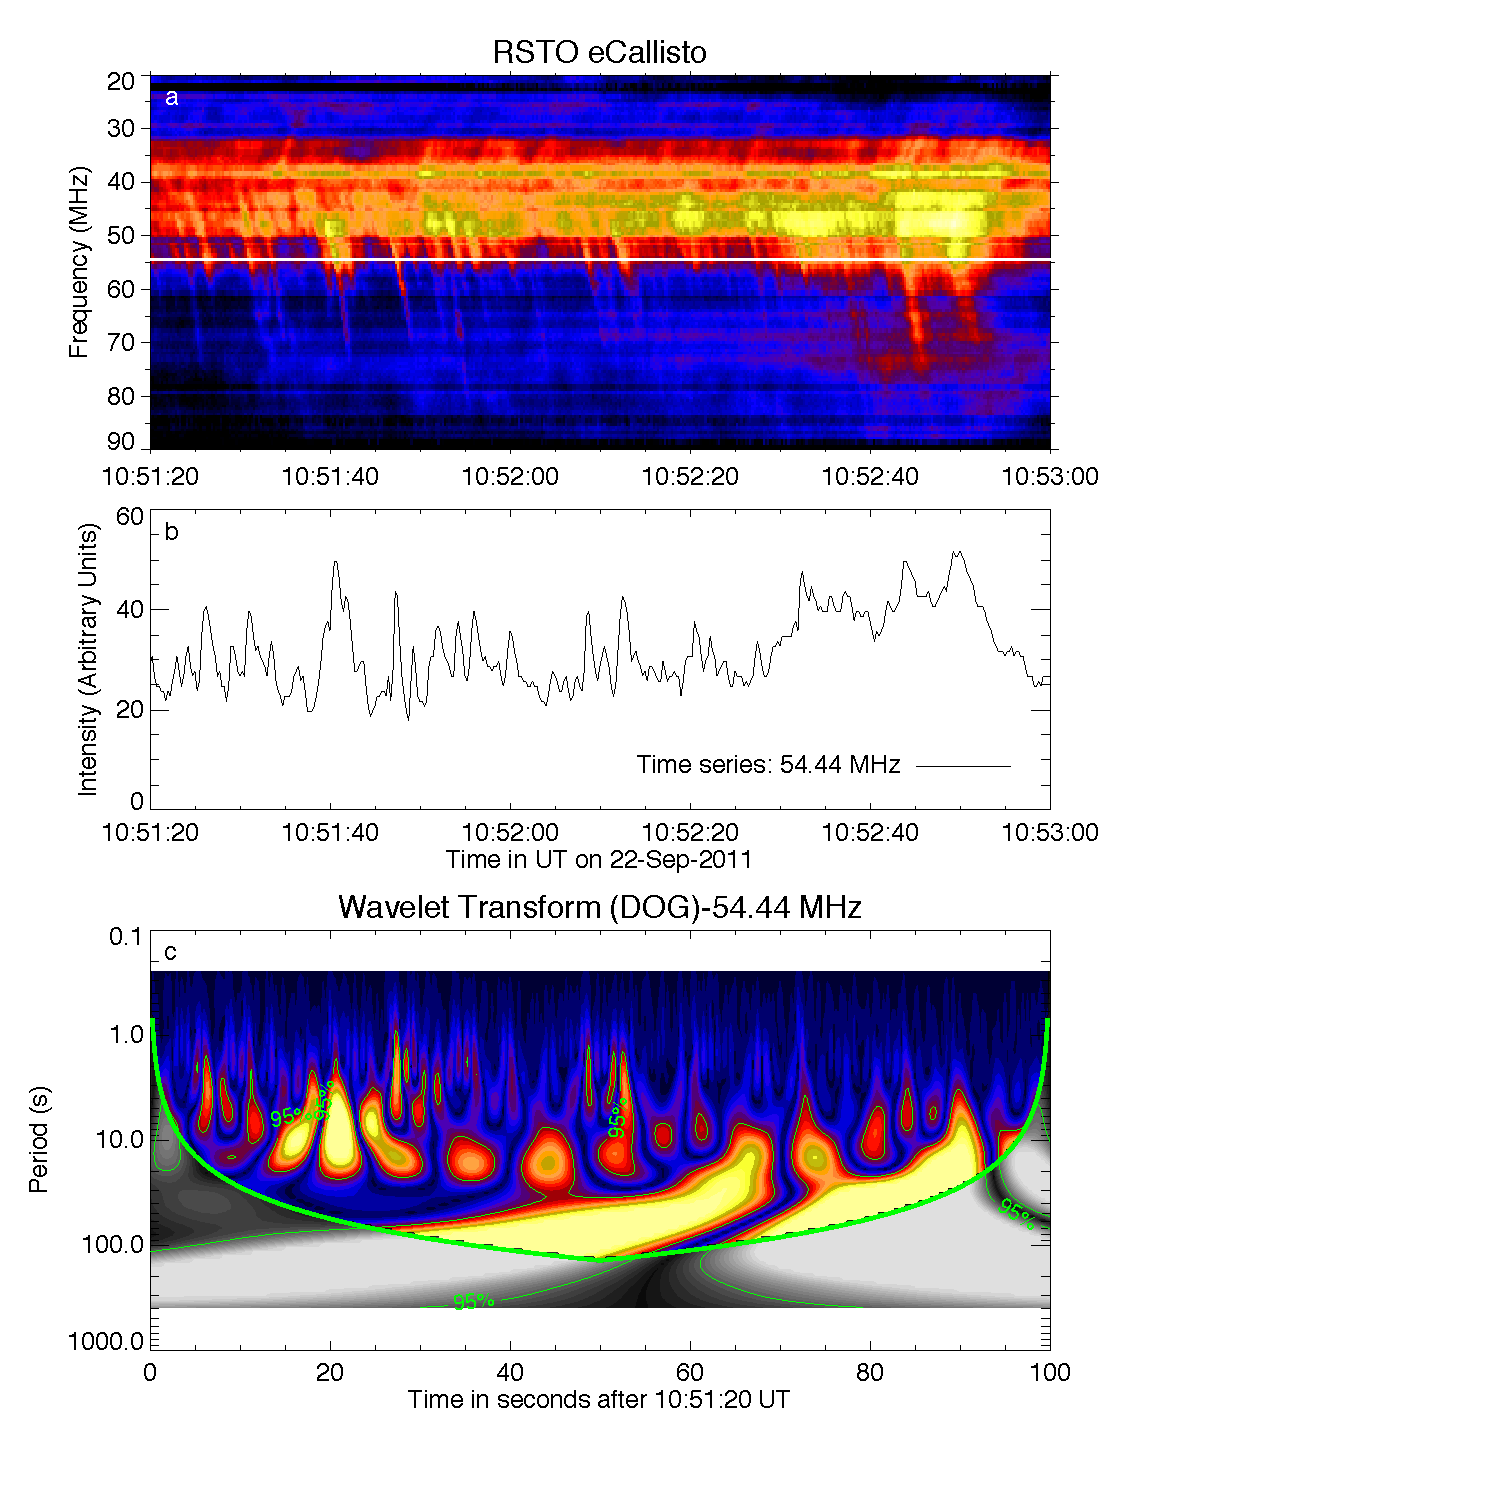
\includegraphics[scale=0.6, trim=0cm 0cm 5cm 1cm]{gallagher_supplem_fig1_final.pdf}
\caption[Herringbone wavelet analysis]{Wavelet analysis of herringbone radio bursts. Panel {\bf a} shows the herringbones, the white line is the frequency from which a time-series has been extracted (54.44\,MHz). Panel {\bf b} shows the time series. Panel {\bf c} shows a wavelet analysis of the time series using a derivative of a Gaussian (DOG) wavelet. The shaded grey area is the region outside the cone of influence and the green contours mark the 95\% confidence level. The wavelet transform shows power in the regions of 2-11 seconds, revealing strong levels of periodicity throughout the time series.}
\label{wavelet}
\end{center}
\end{figure}

While their structure in frequency reveal how fast these beams travel, their behavior in time can reveal detailed temporal characteristics of the shock acceleration process.
A wavelet analysis using a derivative of a Gaussian wavelet performed on a time series at 54\,MHz reveals periodicity at 2--11~seconds (see Supplementary Figure 1). Previous authors have attributed this bursty nature to rippling and inhomogeneity along the shock front, possibly revealing some level of instability or shock turbulence in the acceleration region \citep{burgess2006, guo2010}; we discuss this in the last section. We note that the features at 100--200\,MHz appear to be the extension of the herringbones into higher frequencies. These features in particular show good temporal correspondence with the radio source i.e., they have a start-stop time comparable to the radio source. This is particularly apparent for the group of bursts at 10:52--10:56\,UT.

The radio emission in the dynamic spectra have all the hallmarks of shock generation with particle acceleration closely tied to the process. The association of shock radio activity with the imaged 150\,MHz source suggests that the two observables have a common origin in a plasma shock. Overall, the position of the radio source at the southern flank of the CME, the transverse motion of the source (propagation parallel to the surface) and the zero frequency-drift of the herringbones is suggestive of a shock driven parallel to the surface by the flank expansion, similar to the assertion by \cite{stewart1980} and \cite{schmidt2012}. Indeed the association of the CBF with this radio activity is corroborative evidence of the wave/shock system at the flank. Further evidence of a shock having occurred in the corona was obtained through white-light observations, allowing us to study the position of this shock relative to the CME.

\section{White-light CME and Shock}
\begin{figure}[!t]
\begin{center}
\includegraphics[scale=0.6, trim=2.5cm 1cm 0cm 1.5cm]{gallagher_figure4_final.pdf}
\caption[3D reconstruction of CME and white-light shock]{White-light CME observations and 3D reconstruction of the CME front. {\bf a} Top-down view of the Heliocentric Earth Equatorial (HEEQ) system, showing the separations and locations of STEREO-B and SOHO spacecraft with respect to the Sun. {\bf b} LASCO/C2 base-differenced image of the CME (logged intensity scale), with AIA 21.1\,nm image inset. White crosses indicate a point-and-click along the CME front with a corresponding ellipse fit in blue, where the solid lines indicate the major and minor axes, while dashed lines indicate the apex points back toward the Sun centre. The white circles indicate the white-light shock. The red asterisk points indicate the northern and southern flanks of the CME. {\bf c}, Base difference image of the CME from the COR1-B coronagraph, with a corresponding ellipse fit and EUVI 19.5\,nm image inset. The red lines are the red asterisk points in {\bf b} projected as lines-of-sight across the COR1 field of view. {\bf d} 3D reconstruction of the CME with the white light shock indicated on the plane of sky (only 2D information is available for this feature). The red dotted lines are the projected points from the ellipse on the C2 image, and the blue dotted lines are the projected points from the ellipse on the COR1 image. The black ellipses are those inscribed in the resulting quadrilateral slices via the elliptical tie-pointing method for 3D CME reconstruction, as described in \citep{byrne2010}.}
\label{fig:3d_cme}
\end{center}
\end{figure}
A CME associated with this event was observed by the Large Angle Spectroscopic Coronagraph \citep[LASCO;][]{bru95}, first appearing at 10:46\,UT, with an apex heliocentric distance of $\sim$2.6\,$R_{\odot}$ (Fig.~\ref{fig:figure_aia_nrh_c2}c). The next available image shows the bright CME front with a fainter, secondary front at the southern flank (Fig.~\ref{fig:wl_shock}b). This `two-front' morphology is a common occurrence in white-light CME structure and constitutes a reliable signature of a CME front associated with a stand-off shock \citep{vourlidas2012}. In order to distinguish between the CME front and shock front, we performed a 3D reconstruction of the CME using the elliptical tie-pointing method described in \cite{byrne2010} (Fig.~\ref{fig:wl_shock}d). 

This reconstruction reveals that the bright front outlined in the C2 coronagraph (ellipse in Fig.~\ref{fig:wl_shock}b) corresponds to the faint front outlined as a halo in STEREO-B COR1 (ellipse in Fig.~\ref{fig:wl_shock}c). Furthermore, the observations reveal that the secondary and extremely faint front at the southern edge of the CME (as imaged in LASCO/C2,~Fig.~\ref{fig:wl_shock}b) cannot be considered as part of the CME structure, but is actually an associated shock front. We note that white-light shocks have been reported in the past, occurring both in the low corona as well as out to $\sim$0.5\,A.U. \citep{vourlidas2012, maloney2011}. Here, we have employed a 3D reconstruction from multi-viewpoint observations to qualitatively confirm the presence of a shock at the southern flank of the CME, in the same region as the CBF and radio burst. Finally, a height time analysis of this CME showed that there was no acceleration in the C2 and C3 fields of view, with the CME having a constant velocity of $\sim$1300\,km\,s$^{-1}$.


\section{Discussion}

\subsection{Relationship Between CME, CBF, and Radio bursts}\label{sec:31}

There has been much debate surrounding the assertion that CBFs are a wave phenomenon \citep{gallagher2011}, with numerous authors suggesting a pseudo-wave theory \citep{delannee2008}. In the past, the association of CBFs with type II and type III bursts has been used as evidence against this pseudo-wave interpretation and more in favor of the MHD wave paradigm \citep{warmuth2004b, grechnev2011}. This study reveals that the CBF in this event was indeed closely associated with shock radio activity positioned on the flanks of an expanding CME. This kind of behavior has been suggested before, but never directly imaged \citep{kozarev2011, feng2012, feng2013}. It shows how a combination of radio and EUV imaging can reveal the evolution of plasmoid driven shocks in the solar atmosphere \citep{bain2012}.

The scenario shown to be the case here, is that the expansion of the CME flanks drove a plasma pressure front through the corona. The low coronal manifestation of this pressure front was a CBF. Higher in the corona this same pressure front steepened into a shock; this shock was responsible for the acceleration of particles. These particles produced radio emission which was observed as a propagating radio source and in dynamic spectra in the form of herringbones. Such a scenario is agreement with a variety of studies that have suggested such a physical mechanism e.g., the schematic of \citep{grechnev2011a} shown in Figure~\ref{fig:shock_cbf}, Figure 7 of \citet{warmuth2004b}, and Figure 3 of \citep{stewart1980}. Our own schematic shows a similar scenario in Figure~\ref{fig:shock_schematic}.

\subsection{Bursty Particle Acceleration}\label{sec:sda_discussion}

Of further interest in this study is the likelihood of a quasi-perpendicular orientation of the shock, as revealed by the PFSS extrapolation. A schematic of the CME, CBF and shock orientation with respect to the coronal magnetic field and particle acceleration is shown in Figure~\ref{fig:shock_schematic}
\begin{figure}
\begin{center}
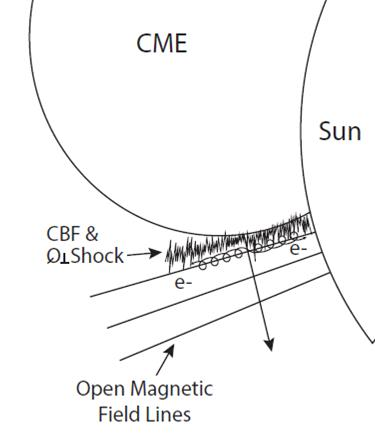
\includegraphics[scale=0.7]{gallagher_schematic.png}
\caption[CBF and shock orientation]{Relationship between the CME, CBF, shock and particle acceleration on the open magnetic field of the ambient corona.}
\label{fig:shock_schematic}
\end{center}
\end{figure}
Quasi-perpendicularity is an essential aspect of the shock drift acceleration (SDA) mechanism \citep{ball2001}, a process believed to be responsible for particle acceleration in planetary magnetospheres \citep{wu1984} and solar radio bursts \citep{holman1983}.
This mechanism involves an adiabatic reflection of particles from the shock, with the energy gain sourced in the $\mathbf{V} \times \mathbf{B}$ electric field, where $\mathbf{V}$ and $\mathbf{B}$ are the upstream flow speed and magnetic field, respectively. A single reflection from the shock has limited energy gain, however multiple reflections may produce relativistic energies, which is particularly important for low Mach number shocks such as that reported here ($M_A =2.4^{+0.7}_{-0.8}$) and in \citep{guo2012}. This multiple reflection process may be explained by inhomogeneity in the shock front, a characteristic usually known as \textquoteleft rippling' \citep{zlobec1993, vandas2011}. 2D hybrid simulations show that rippling is brought about by an instability \citep{burgess2006} and resembles a standing-wave mode of the shock surface \citep{lowe2003}. The presence of ripples can lead to a quasi-sinusoidal variation in shock-normal orientation with respect to the upstream magnetic field. Since the efficiency of SDA requires quasi-perpendicularity, there will be sites on the shock front that provide efficient acceleration and sites that do not $-$ a structure that may lead to magnetic trapping and multiple reflections \citep{zlobec1993}, hence producing higher energy particle acceleration. 

The presence of ripples can produce quasi-periodic herringbones in three ways. Firstly, it makes SDA more efficient and capable of producing the observed herringbone energies, especially when particle scattering is considered \citep{burgess2006}. Secondly, the periodic spatial variation in the acceleration efficiency of the shock could explain the bursty and quasi-periodic nature of the herringbones. \cite{guo2010} suggest that shock front inhomogeneity brought about by MHD turbulence is a possible explanation of bursty herringbones. \cite{schmidt2012} produced a detailed model of SDA from a rippled shock, specifically on the flanks of an expanding CME. Their results suggest that herringbones could be produced by accelerated electrons at spatially intermittent regions of quasi-perpendicularity on a rippled shock surface (Figure~\ref{fig:herbone_model}). Thirdly, \citep{burgess2006} also predicts that, if rippling is present, the upstream and downstream electron beams should have similar energies, which is not predicted for a uniform or \textquoteleft smooth' shock. A sample of the oppositely drifting herringbones in Fig.~\ref{fig:dyn_spec}c shows that positive and negative frequency drifts are both $\sim$5\,MHz\,s$^{-1}$, revealing that the upstream and downstream populations have similar energies (although we note the possibility that both positive and negative drifting herringbone features may be accelerated upstream, as suggested by the schematic of \citep{zlobec1993}). There is also the possibility that the herringbones may be associated with a termination shock of a reconnection outflow occurring behind the CME \citep{aurass2004}. In such a scenario, this shock would have a more indirect relationship with the CME propagation. However, the imaged radio source shows a good temporal correspondence with the shock activity in the dynamic spectra, especially between 10:52$-$10:56\,UT, suggesting the particle acceleration indicated in the spectra shares a close relationship with the propagating source.

Our observations reveal the need for a more detailed modeling of herringbone solar radio bursts. The quasi-periodic behavior of herringbones provides a possible direct measure of shock inhomogeneity and the spatial scales over which the magnetic field varies in the shock and ambient corona; it may also provide a measure of the turbulence in these plasma flows \citep{guo2010}. In the future, high cadence EUV imaging from SDO, combined with sensitive radio imaging-spectroscopy observations from instruments such as the Low Frequency Array \citep[LOFAR;][]{vanHaarlem2013}, will reveal unprecedented detail of plasma shocks and their role in particle acceleration. This may reveal the fundamental nature of a plasma shock process that is universal, but currently impossible to directly observe in any other area of astrophysics. 



%!TEX root = ../thesis.tex
%Adding the above line, with the name of your base .tex file (in this case "thesis.tex") will allow you to compile the whole thesis even when working inside one of the chapter tex files

\singlespacing
\chapter{Conclusions and Future Work} 

\label{chap:6}

\doublespacing
The first goal of the this thesis was to derive CME masses from observation that have the smallest and most reliable uncertainty to date, and to use this information to calculate a better estimate of CME energies and the first observational quantification of the Lorentz force acting on a CME.
The second goal of this thesis was to increase the understanding of the relationship between CMEs, CBFs and radio bursts. This was achieved through evidence for a shock driven by a CME flank, resulting in the CBF and type II, type III, and herringbone radio bursts. n this chapter, I will summarise and conclude this research and outline the future of this study
\clearpage

\section{CME Masses and Energies}

\subsection{Principle results}

The goal of the this thesis was firstly to derive CME masses from observation that have the smallest and most reliable uncertainty to date. This was achieved using the two vantage points of the STEREO Ahead and Behind spacecarft, allowing CME geometry, and the associated mass underestimations, to be fully characterized. This then allowed a better estimate of CME energies and the first observational quantification of the Lorentz force acting on a CME. The principle results are as follows:
\begin{itemize}
\item The first assumption of nearly all CME investigations is that the CME is confined to the 2D sky-plane. These leads to two sources of mass underestimation which primarily arise from the geometrical sensitivity of the Thomson scattering equations for the solar atmosphere. Firstly, if the CME propagates propagates at some angle away from the sky-plane, but we do not take into this angle into account, then we will underestimate the mass. Knowledge of the propagation angle from STEREO A and B observations allows us to eradicate this uncertainty. Secondly, all CME material is confined to a 2D plane at some angle $\theta$. This underestimation cannot be eradicated but we can characterise its effects by simulating a CME with angular width $\psi$ and homogenous density distribution. This allows an estimate of the simulated observed mass and a comparison of this to the actual mass. For any CME width $\psi$ at a sky-plane angle $\theta$ we may calculate the CME mass underestimation when we deproject the CME mass onto its plane $\theta$. A surprising result from this is that for all angular widths $\psi$, deprojection estimates exactly the CME mass when propagation is at an angle $\theta=60^{\circ}$.

\item In the past CME mass uncertainties from the geometrical unknowns described above were either extremely large at more than 50\% \citep{vou00} or entirely unquantifiable. Adding to this all the other sources of uncertainty (coronal composition and interactions with streamers) results in CME mass estimates that are entirely unusable in a scientific analysis. With the capabilities of the STEREO spacecraft, the geometrical mass uncertainties of the CME occurring on 12 December 2008 were reduced to 10\%, a dramatic improvement over previous results. The biggest source of uncertainty was the interaction of this CME with a streamer, adding a further 15\%. Taking everything else into account the final mass uncertainty came to 30\%, which is both smaller and more reliable than any uncertainty given previously. The final total mass of the CME came to
$3.4\pm1.0\times10^{15}$\,g, perhaps the only quotation of mass with an uncertainty in the literature. In an ideal case of a CME that has no background streamer interactions the uncertainty could be reduced even further.

\item This research included the first quantification of the Lorentz force acting on the CME during its early phase propagation. At $3.4\pm2.2\times10^{14}$\,N, it was shown that this is the most dominant force on a CME at $3\,R_{\odot}$, being greater than gravity and drag due to the solar wind. This is the first direct evidence for Lorentz force dominated dynamics, which has been only indirectly shown in previous studies \citep{bein2011}. The quantification of this force is also important for constraining parameters of MHD models of CMEs. There are a variety of models of CMEs which successfully describe formation of a flux rope and its eruption into interplanetary space. These models employ a number of forces, given by the MHD momentum conservation equation, to propel the CME out of the low corona. The most important of these forces for doing work against the Sun's gravitational potential is the Lorentz ($\mathbf{j}\times\mathbf{B}$) force. While all models include a Lorentz force treated explicitly through currents and magnetic fields, or implicitly only through magnetic field, the sizes of the force in the models is entirely unconstrained. MHD models of CMEs have the freedom to choose any size Lorentz force because no work had been done on the actual size of this force. For example, \citep{chen1996} predicts a Lorentz force of X\,N during early phase propagation. This would seem to orders of magnitude too high, and further observational investigations of the forces on CME may show this.

\end{itemize}

\subsection{Future Work}

\subsubsection{CME Mass and Energy Catalogue}

There are a variety of catalogues that list CME times and kinematics for all events detected by LASCO up to the present time (REFERENCES). None of these catalogues include any measure of CME masses. This is possibly due to the difficulty in unambiguously identifying the CME in coronagraph images. A current investigation is underway to test the feasibility of automatically calculating all the masses of all CMEs in the LASCO catalogue. Such an endeavor would require accurate detection of all CME material in the images. The automatic detection routines under development by Byrne are a possible candidate to employ automatic mass calculation routines. The Byrne algorithm has the possibility of providing masks for the total CME area such that a summation of its mass content may be achieved. These masks are shown in Figure~\ref{fig:masks}. These masks use multi-scale filtering to detect the area of the CME in the image. A conversion of the image to pixel values of grams, as described in Chapter 4, and summation of the all pixels would yield the total CME mass.

\begin{figure}[h!]
\begin{center}
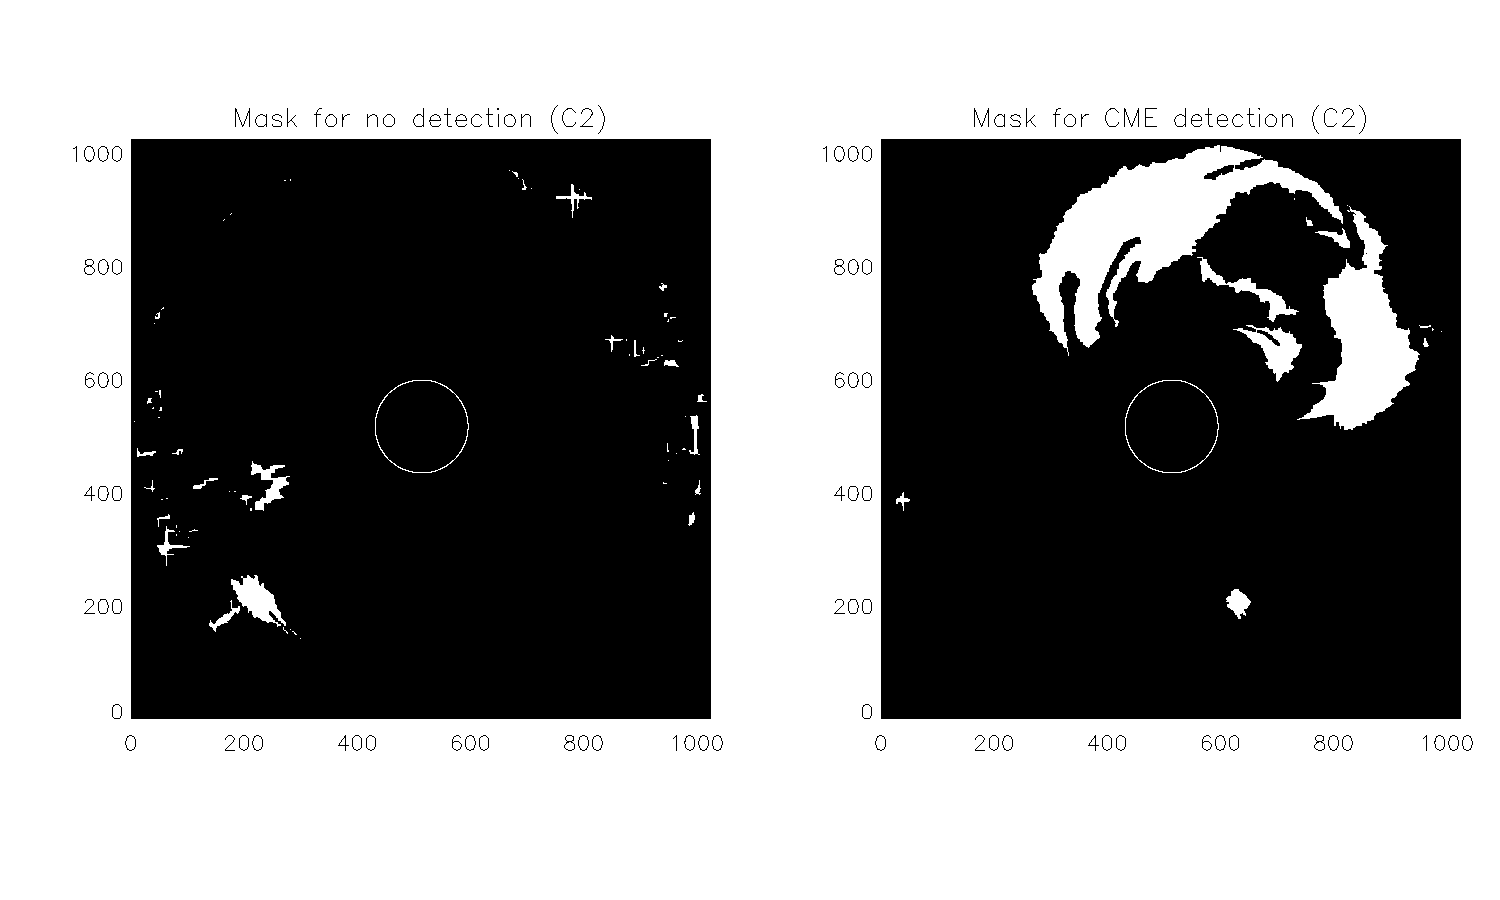
\includegraphics[scale=0.6, trim=2cm 2cm 1cm 1cm]{masks.pdf}
\caption{Sample C2 masks for no-detection (left) and CME-detection (right). The no-detection masks has some spurious blobs, possibly due to cosmic rays and small ejections of plasma. The CME detection covers most of the CME body, but masks the center due to presence of CME core? Circle shows solar limb.}
\label{fig:masks}
\end{center}
\end{figure}
%----------------------------------------------------%
%			  Describe method
%
The method was tested on a particularly active period of CME eruptions from 25 April 2010 to 2 May 2010, observed by LASCO C2 and C3. The detection mask was applied to each image in the sequence between the dates. In the majority of images there are no detections (Figure~\ref{fig:masks}(left)) and if a CME is in the image it will be exposed in a mask similar to Figure~\ref{fig:masks}(right). Each image is base differenced and converted to pixel values of grams using the sky-plane assumption. The pixels are summed such that one image represents one mass value for each image in the sequence i.e., the image sequence allows us to calculate a mass time-series, shown in Figure~\ref{fig:mass_v_time}. The top panel shows a mass time series on a linear scale, the CME detections of a standard $\sim$$10^{15}$\,g can be seen in the time series of both C2 and C3. The method is quite successful in calculating a reasonable mass value for moderate to large CMEs ($\sim$$10^{15}-10^{16}$\,g). 
%----------------------------------------------------%
%			       Initial trial
%
A more appropriate representation is given in Figure~\ref{fig:mass_v_time}\,(lower), where the y-axis is logged. Realistically, all of the mass plots should be logged given that CME masses tend to span approximately two orders of magnitude ($10^{14}-10^{16}$\,g). As can be seen in Figure~\ref{fig:mass_v_time}\,(lower), logging the axes reveals a detection of a large background mass even during a quiet time of no CME detection. The background or `quiet-time' values are $\sim$10$^{14}$\,g or slightly higher. This is reasonable for average to large CMEs ($10^{15}-10^{16}$\,g), but the smaller CMEs with $\sim$10$^{14}$\,g will be completely masked by the quiet-time detections. The effect of detecting quiet-time mass also may introduce what seem to be CMEs i.e., a false detection. At the start of the plot between 25 April - 26 April, the LASCO C2 curve (blue) appears to have detected a CME of $\sim4\times10^{14}$\,g, however this is a quiet period with no CME detection. The background mass values result from an imperfect mask during quiet times. Even though there is no CME, the mask may still detect small clumps and blobs of solar wind that show up as positive areas in the binary mask Figure~\ref{fig:masks}. A current line of investigation to elimate this is to only accept detections greater than a certain angular width. Since CMEs tend to be $>40^{\circ}$, anything below this should be rejected and zeroed in the mask.
%
%
\begin{figure}[h!]
\begin{center}
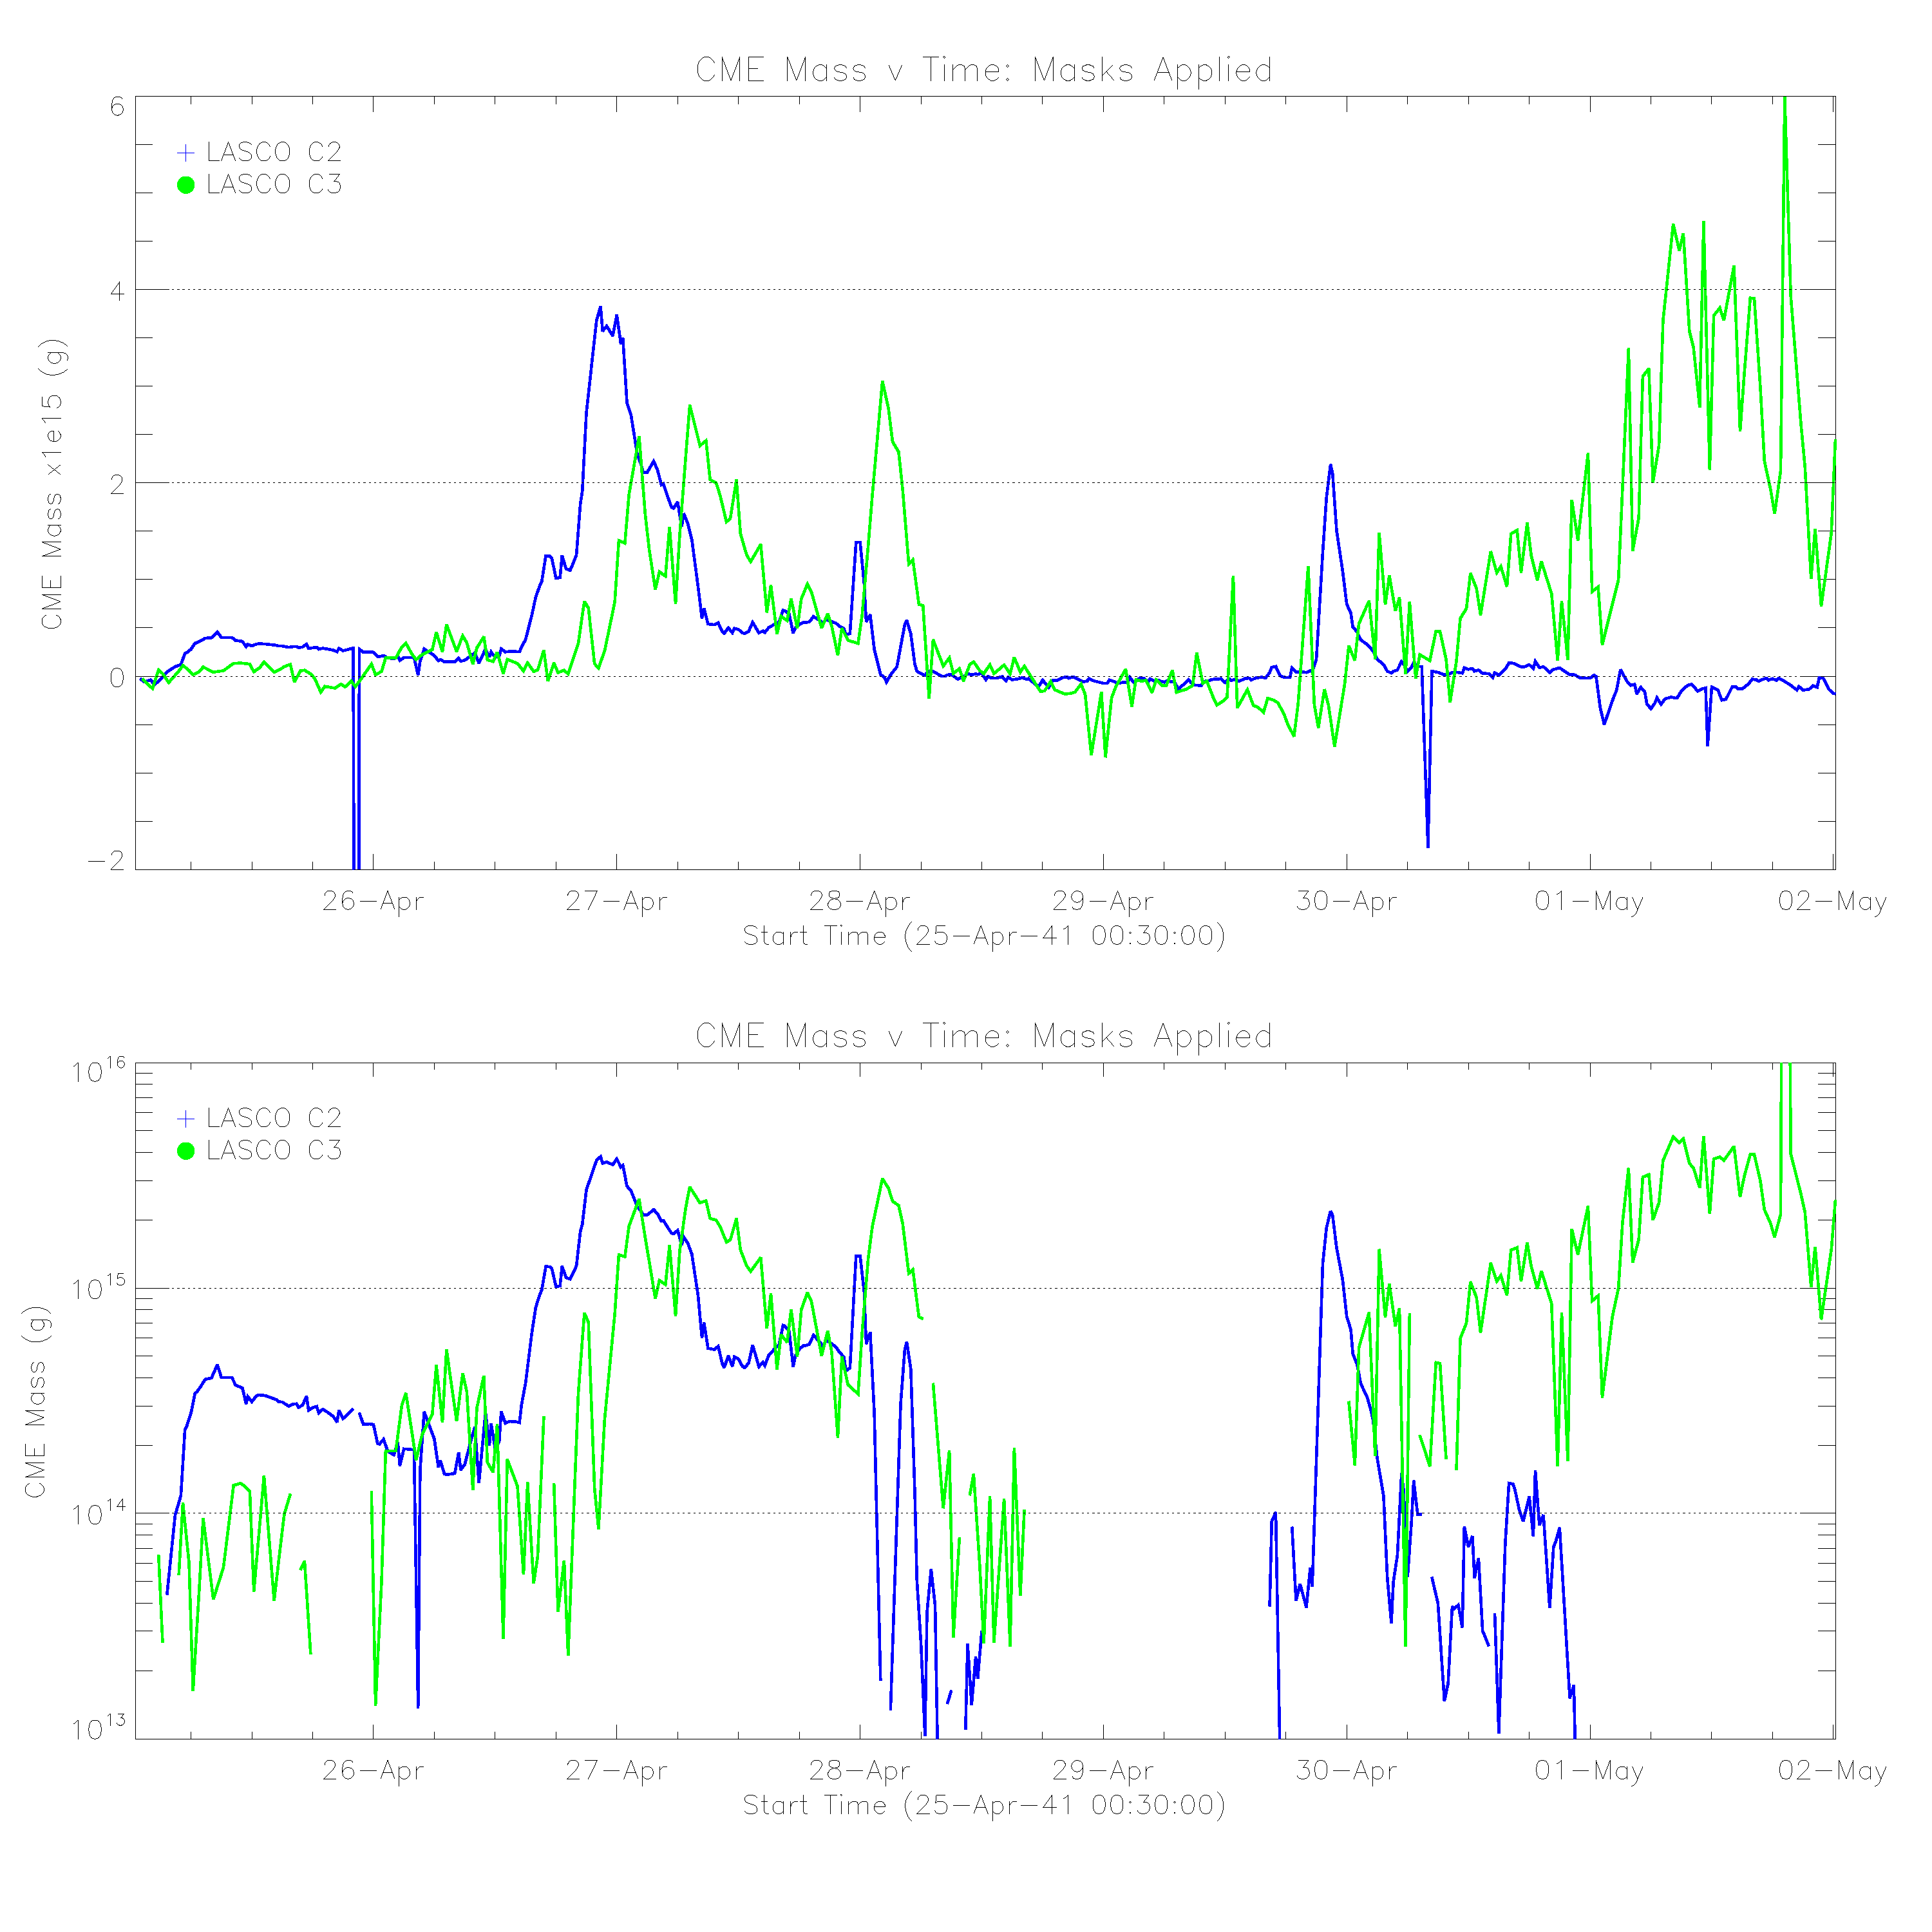
\includegraphics[scale=0.3, trim=7cm 2cm 7cm 4cm]{CME_MASSES_lin_log}
\caption[CME Mass automatic detection]{(Top) Mass estimates calculated using LASCO C2 and C3, and the detection masks of CORIMP. All images in the seven day observation sequence have been base-differenced, with the first image in the sequence used as a pre-event image. Representing mass on a linear scale shows clearly that the method results in reasonable estimates of CME mass. All CMEs are assumed to be propagating on the plane of sky (POS). 
(Bottom) Same data as Figure 1, with a logged y-axis. Logging the y-axis is more appropriate, given that CME masses tend to span approximately two orders of magnitude $10^{14}-10^{16}$\,g. However, with the logged axis, some issues with the method are highlighted e.g., the CME detection masks tend to capture spurious blobs (mass ejections, but not quite big enough to be regarded as CMEs). These blobs seem to occur in a lot of frames, making the background `quiet detections' level sit at $\sim$10$^{14}$\,g or higher. This is ok for larger CME masses however, the smaller CMEs with $M_{cme}\sim$10$^{14}$\,g will be swamped by this background detection. If we are to detect the whole range in mass, this background will have to come down. }
\label{fig:mass_v_time}
\end{center}
\end{figure}
%
%
%
%----------------------------------------------------%
%	 	Problem with background
%
There are a number of test which need to be performed in order to check that (i) the background subtraction is appropriate (ii) the mask has detected the right quantity of CME mass. At the moment the first image in the observation sequence is subtracted from all subsequent images. Not ideal, given that a CME eruption will change the background corona substantially. To avoid using the very first image, an algorithm needs to be employed to recognize a period of inactivity prior to eruption, and use an image (or an average of images) from this quiet period in the subsequent base difference.
%----------------------------------------------------%
%	 	 Test of the masking method
%
To check that (i) and (ii) are fulfilled we employ the fact that the following must be true
\begin{equation}
M_{mask} = M_{no\_mask} - M_{inverse\_mask}
\end{equation}
where $M_{mass}$ is mass calculated with the mask applied as normal, $M_{no\_mask}$ is just the total array summed, and $M_{inverse\_mask}$ is the CME masked with the remainder summed. The inverse mask is in Figure~\ref{fig:inverse_masks}. 
\begin{figure}[t!]
\begin{center}
\includegraphics[scale=0.6, trim=0cm 2cm 0cm 0cm]{inverse_masks}
\caption{The inverse mask, allows everything \emph{but} the CME to be summed. Black circle is solar limb.}
\label{fig:inverse_masks}
\end{center}
\end{figure}

\begin{figure}[t!]
\begin{center}
\includegraphics[scale=0.3, trim=0cm 2cm 0cm 1cm]{compare_masks_c2c3}
\caption{Time series of the mass obtained from using no mask and using the inverse mask. The data behave as expected, with the inverse mask being essentially the same as the no-mask but smaller by the CME mass. The drift towards negative values is symptomatic of a pre-event image (for base-difference) that is too bright. The discontinuous values are due to badly prepped images in the NRL archive.}
\label{fig:inverse_masks}
\end{center}
\end{figure}
We perform the time series again to calculate $M_{no\_mask}$ and $M_{inverse\_mask}$, shown in Figure~\ref{fig:inverse_masks}. They behave as expected, with the inverse-mask being essentially the same as the no-mask, but smaller by a roughly constant amount; this roughly constant amount should equal the CME mass. The effect of a single pre-event image used in the base-difference for the whole sequence is very apparent. In both C2 and C3 the masses grow toward increasingly negative values. This happens because the pre-event image is too bright and is a bad representation of the background corona over the observation sequences. In the intervening hours between start and end time a number of CMEs erupt. This will result in a dimming of the background corona over time as the corona becomes depleted or evacuated. This method has determined that condition (i) is not fulfilled, and is a good error check to see if an appropriate background has been chosen. To test condition (ii) we compare the difference of the blue and orange time series in Figure~\ref{fig:inverse_masks} with the time series calculated using the normal mask, the results are shown in Figure~\ref{fig:comparison}. The trends in both time series match, however they diverge as time increases. 
\begin{figure}[t!]
\begin{center}
\includegraphics[scale=0.3]{mask_nomask_invmask_c2c3}
\caption{Comparison of the mass from masked images (blue) the no\_mask - inverse\_mask images (red) for C2 (upper) and C3 (lower). For both C2 and C3 the blue and red lines are a good match. The most obvious difference is the positive drift of the red line in C2, due to an excess background brightness subtracted in the base-differencing.}
\label{fig:comparison}
\end{center}
\end{figure}
The over-bright pre-event image used in the base difference is drawing the background values in no-mask and invert-mask into negative values. The blue line in Figure~\ref{fig:inverse_masks} (upper panel) should sit at zero, while the orange line should only show positive values when a CME is in the frame. The fact that they both drift into the negative means they will result in a positive excess when subtracting the two.
Algebraically, the procedure resulting in the red line in Figure~\ref{fig:comparison} is as follows:
\begin{equation}
y = (img - pre) - (img - pre)\times mask_{inverse}
\end{equation}
where $img$ is the current image and $pre$ is pre-event image; $img - pre$ represents a base difference. $mask_{inverse}$ is the inverted mask e.g., Figure~\ref{fig:inverse_masks}. Ideally, equation (2) would result in
\begin{equation}
y = M_{cme} - 0
\end{equation}
However due to excess brightness in the pre-event image we end up with a negative mass value $M_{neg}$ combined with the cme mass $M_{cme}$
\begin{equation}
y = (M_{neg} + M_{cme})  - M_{neg}
\end{equation}
Since $M_{neg} < (M_{neg} + M_{cme}   ) < 0$, we end up with $y$ value that is positive and larger than $M_{cme}$. Of course, if the pre-event image were chosen appropriately we would just have equation (3), no problem. It's interesting to note that the difference between the blue and red line in Figure~\ref{fig:comparison} is a measure of how much the background corona changed over time; it also a measure of how well chosen the background image is for the base-difference. If the lines diverge consistently, too much background brightness has been extracted from the images. The effect is not as pronounced in C3 for the observation sequence, probably because the CME does not perturb the background corona at this height range as much as it does at lower heights (in C2 FOV). Hence the analysis resulting in Figure~\ref{fig:comparison} are a way of confirming that criteria (i) and (ii) are fulfilled.

There are a number of questions and issues that need to be addressed if the automatic mass detection is to produce reliable results:
\begin{itemize}
\item Removal of the spurious blobs in the quiet-time masks. Background values need to be brought to a maximum of $10^{13}$\,g, this will ensure detection of even small CMEs with masses of $\sim$$10^{14}$\,g. A criteria for the removal of these blobs could be to ignore detections smaller than a threshold angular width i.e., set to zero all features with angular width $<40^{\circ}$
\item An algorithm to choose an appropriate prevent image needs to be implemented. An average of a set of quiet images before CME detection is a possibility. In this case the algorithm will need to identify a CME start time and then to check for the presence of quiet images before this start time. 
\item What mass value should be taken as being representative of the CME mass? Is it appropriate to take the maximum mass value detected during the time interval when the CME is present? If so, should the maximum mass be taken from C2 or C3?
\end{itemize}
The last item here will require a a number of tests to be performed on which telescope can provide the most reliable mass estimate. Primarily, C3 would seem like the most appropriate, since the large field-of-view (FOV) can contain all CME material i.e., there will be none hidden by the occulter, as can happen in the C2 FOV. However, C3 is more susceptible to plane-of-sky (POS) errors e.g., if CME is not actually on POS, the uncertainties introduced by assuming it \emph{is} on POS are worse for C3. There main pros and cons of each coronagraph are
\begin{itemize}
\item C2 \hfill \\
-Pro: CME is closer to POS \\
-Con: Mass is hidden behind disk
\item C3 \hfill \\
-Pro: FOV is large enough to view all CME (smaller mass-hiding)\\ 
-Con: Very bad POS effects
\end{itemize}
These may be addressed by a study of the Thomson scattering geometry of the light received by each telescope.

Finally, the inherent uncertainties on the CME mass a the most serious threat to the feasibility of automatic mass detection. Realistically, we can only give an order of magnitude estimate e.g., CME mass is somewhere between $10^{14}-10^{15}$\,g or $10^{15}-10^{16}$\,g etc. One idea is a CME mass classification into ranges such as
\begin{itemize}
\item A Mass: $10^{13}-10^{14}$\,g
\item B Mass: $10^{14}-10^{15}$\,g
\item C Mass: $10^{15}-10^{16}$\,g
\item C+ Mass: $>10^{16}$\,g (on the off chance that mass is slightly above C)
\end{itemize}
With such a system you could say there was a \textquoteleft C' mass CME on such a date and time, without having to quote some uncertain mass estimate. The uncertainties might result in the mass transcending two classes, in that case you could then quote \textquoteleft BC' mass. In practice, such large ranges may be the only way in which CME mass values can be presented in a catalogue. Despite such limitations, this may be useful to any user wishing to search for events that have small, intermediate, or large energies.

\subsubsection{Mass Estimates with AIA}
\begin{figure}[t!]
\begin{center}
\includegraphics[scale=0.35, trim=1cm 0cm 0cm 1cm]{euv_dimming.png}
\caption[EUVI dimming region]{EUV dimming region observed by EUVI 195\,\AA~channel on 31 December 2007. The dimming is due to evacuation of plasma from the region such that the emission measure drops \citep{aschw09}}
\end{center}
\end{figure}
Despite the fact that there a number of studies that have determined the mass of CMEs with varying degrees of uncertainty, very few studies have investigated where exactly the CME mass comes from. The origin of the mass is difficult to determine since by the very early stages of CME development are obscured by the occulting disk of a coronagraph. This means that EUV imagers of the corona are currently the only viable method of observing the birth of a CME. The presence of a CME in such observations are usually conspicuous by a lack of emission i.e., as the CME erupts it evacuates an active region, leaving behind an emission deficit. This emission deficit is known as an EUV `dimming' region and has been used to calculate the amount of evacuated mass \citep{aschw09}. Dimming regions are also a regular feature of soft X-ray images \citep{sterling1997}.

The method of \citet{aschw09} exploits the fact that there are multiple filters in EUV that can be used to measure the amount of evacuated mass in dimming regions. The evacuated mass from the dimming region, $m_d$, may be calculated from
\begin{equation}
m_d(t,T) = m_p n_d(t)V_D = m_p n_A\sqrt{\frac{I_d(t)}{I_A}}\frac{\pi}{4}w_d^2\lambda_T
\end{equation}
where $m_p$ is proton mass, $n_d$ is dimming number density, $V_D$ is dimming volume, $n_A$ is active region density (pre eruption), $I_d$ is dimming region intensity, $I_A$ is active region intensity (pre-eruption), $w_D$ is the radius of the circular footprint of the dimming region, and $\lambda_T$ is the temperature scale height. Since $m_d$ may be measured in each of the temperature filters of the EUVI imager the total mass may be constructed from a differential emission measure-type mass distribution
\begin{equation}
m_{cme}(t)=\int_{T_1}^{T_2}\bigg( \frac{dm_d(t,T)}{dT} \bigg)dT = \int_{T_1}^{T_2}\frac{\Delta m_D}{\Delta T_F}\mathrm{exp}\bigg( -\frac{(T-T_0)^2}{2\sigma_T^2} \bigg)dT
\label{eqn:tot_euv_mass}
\end{equation}
This analysis has been performed for EUVI on STEREO A and B. This imager only has three different passbands at 171\,\AA, 195\,\AA, and 284\,\AA, representing only three data points to which a gaussian is fit to the mass temperature distribution (Figure~\ref{fig:euvi_mass}).
\begin{figure}[t!]
\begin{center}
\includegraphics[scale=0.56, trim=1cm 0cm 0cm 1cm]{mass_temp_dist.png}
\caption[Mass-temperature distribution]{Mass-temperature distribution from EUVI/A and B for five different events. The three channels if EUVI, 171\,\AA, 195\,\AA, and 284\,\AA, are used to calculated the mass of the material contributing to emission in each of these channels. A construction of a Gaussian using these three measurements allows integration over temperature to find the total CME mass in the temperature range of 0.5--3.0\,MK. \citep{aschw09}}
\label{fig:euvi_mass}
\end{center}
\end{figure}
Since this may be done over time for each EUV image in the observation sequence, a mass evacuation curve may be constructed over time (Figure~\ref{fig:mass_dim_time}). The curves correspond to different flares. This kind of analysis has the ability to give information on the eruption rate of the CME and possibly the forces acting on the ejection. However, not much work has been done in this are and the field is relatively under-explored. A number of interesting questions need to be investigated for for mass evacuation rates:
\begin{itemize}
\item Does mass evacuation rate depend on flare size?
\item Does evacuation rate depend on flare rise-time?
\item Is there any correlation with CME kinematical profiles?
\item Are the mass evacuation rate and final mass correlated?
\item Are mass evacuations different for events that have no associated flare?
\item Ultimately, why are some evacuation rates faster than others?
\end{itemize}
These questions need to be investigated if there is to be an advance in understanding the origins of CMEs. However, EUVI observations are limited in this regard.
\begin{figure}[t!]
\begin{center}
\includegraphics[scale=0.55, trim=1cm 0cm 0cm 1cm]{mass_dim_t.png}
\caption[Mass evacuation with time]{Mass evacuation from the dimming region with respect for five selected events. The biggest flare has the fastest mass loss rate but not the biggest final mass. \citep{aschw09}}
\label{fig:mass_dim_time}
\end{center}
\end{figure}
Since there is only three data points to which the Gaussian is fit to this mass-temperature distribution, the results are quite unconstrained and sometimes unreliable. For example, panels 3--8 of Figure~\ref{fig:euvi_mass} are each a bad representation of a Gaussian. This may be due to the CME plasma temperature lying outside the response of the three EUVI channels. Also, the cadence of EUVI may be too slow to capture the very early stages of mass evacuation, which would be needed if a comparison was to be made with an impulsive flare.

The possibility for advancing this kind of study with AIA is very promising. There are at least three main areas in which AIA can advance such research
\begin{itemize}
\item AIA has a possible six passbands that may be used in the mass distribution curve. This will enable a better constraint on the Gaussian in Equation~\ref{eqn:tot_euv_mass}, producing a more reliable total mass estimate than the three passbands of EUVI. Another result that may stem from this is investigating the temperature distribution of CME material, leading to a development in and understanding of CME thermal energies, which are not well understood.
\item The above results could be advanced with the inclusion of UVCS spectroscopy data, which can give CME thermal characteristics from O\,VI, V and C\,III lines out to a height of $4\,R_{\odot}$. A comparison of early and intermediate phase CME temperatures could determine if the CME expands adiabatically, which is another unknown. This is important for investigating how isolated the CME is from the solar wind plasma.
\item Finally, AIA has a 12 second cadence (EUVI has 10 minutes), enabling a calculation of a mass evacuation curve in the very early stages of CME eruption. As mentioned, this will be particularly important for a comparison with very impulsive flares.
\end{itemize}
There are a wealth of physical properties in the early phase of CME eruption that could be answered with AIA. Up until current time, such an analysis has gone relatively unexplored.

\section{Coronal Shocks and Radio Bursts}

\subsection{Principle results}
The second goal of this thesis was to increase the understanding of CM-driven shocks and show the relationship amongst the various shock observables. A combination of white-light, EUV, and radio imaging showed CBFs and radio bursts have a common origin in a shock, and that this shock was driven by the CME flank. The principle results of this investigation were
\begin{itemize}
\item CBFs are closely associated to particle acceleration radio activity. The temporal correlation between CBFs and radio bursts such as type IIs and type IIIs has been highlighted in the past \citep{klassen2000, maia2004}. However, there are very few, if any, direct observations of an association between radio sources and CBFs. \citet{vrsnak2005a} showed a radio source which propagated around the limb in association with a CBF, however any direct comparison between the two features was hampered by the low cadence of EUV imaging. To date, the Carley {\emph et al.} (2013) observation of a 150\,MHz source closely following a CBF is the most comprehensive presentation of the clear relationship between the two features (Figure~\ref{ig:figure_aia_nrh_c2}). It has confirmed that CBFs are inherently associated with radio activity. This radio activity is plasma emission generated by an instability in the presence of electron beams.
\item The kinematics of the radio source was analysed giving a measure of the speed of this source. In order to estimate its Alfv\'{e}n Mach number, we performed density and magnetic field diagnostics of the corona. Density diagnostics were taken from six AIA passbands and LASCO C2, while the magnetic field measurements were performed using a PFSS extrapolation. The combined density and magnetic field maps allowed us to produce an Alfv\'{e}n speed map of the corona (Zucca {\emph et al.} (in prep)). To our knowledge, this was the first time such a map was produced from observations. It provided a reliable means of comparing the source speed to the Alfv\'{e}n speed of the corona in order to estimate the source Alfv\'{e}n Mach number.
\item The density map was also used in the analysis of the radio bursts in the dynamic spectra of S/WAVES, Nan\c{c}ay DA, and RSTO eCallisto. Usually, density models are employed to derive particle kinematics from drift rates in dynamic spectra. However, this can lead to erroneous positions and speeds of the particles producing the radio emission because the density models may be an unreliable description of coronal density profiles. Use of the density diagnostics from observation allowed us to derive much more reliable coronal heights for the radio activity observed in the dynamic spectra
\item Analysis of the dynamic spectra activity showed there was particle acceleration of up to 0.4\,$c$, which manifests in the spectra as type III radio bursts. These speed of these bursts along the parker spiral were used to estimate an ETA of the electrons at the STEREO -B spacecraft. It was found the ETA matched the observed time of arrival quite accurately. Furthermore, the observations of herringbones were the most striking evidence for particle acceleration in this study. The observations of herringbone fine structure were made possible by the installation of RSTO eCallisto spectrometers, as described in Chapter 3. The dynamic spectra from RSTO produced some of the clearest spectra of these herringbone bursts compared to other dynamic spectra observations. An analysis of these bursts showed that they are produced by electrons at a speed of 0.15\,$c$ and occur with a quasiperiodicity of 2-11 seconds.
\item Both the radio source imaged by NRH and CBF had a close association with the southern flank of the CME. Since the a thermal analysis of the CBF showed that it was most likely a pressure wave, and the radio source was associated with spectral shock activity, we conclude that a shock driven by the CME flank expansion was the likely driver of CBF and radio activity. Evidence for a shock at the CME flank also came in the form of white-light observations. These observations were used to reconstruct the CME in 3D dimensions and show that the faint feature observed to the south of the CME in LASCO C2 was not part of the CME structure, and therefore must be shock.
\end{itemize}
Overall, this work has shown how a combination of radio and EUV imaging can reveal the evolution of plasmoid driven shocks in the solar atmosphere. It has shown that CBFs and radio bursts share a common origin in a shock driven by the expansion of a CME flank.

\subsection{Future Work}

\subsubsection{Hough Transform and Herringbone Statistics}
\begin{figure}[t!]
\begin{center}
\includegraphics[scale=0.4, trim=0cm 2cm 3cm 1.5cm]{r_theta_line.pdf}
\caption[Hough transform herringbones]{Herringbone bursts detected using the Hough transform. Note that interpolation between frequency channels in the dynamic spectrum results in strong levels of vertical lines, which represent the overwhelming majority of detections by the Hough transform. The herringbones are a weaker source of straight line detections, hence not all of them are revealed by the transform.}
\label{fig:r_theta_line}
\end{center}
\end{figure}
As mentioned in Chapter 5, the frequency drift of herringbones can give information on the particle speeds, whereas there behaviour over time may depend on the shock acceleration characteristics. Also, the emissivity of plasma emission depends on the velocity of the particles inducing the emission (Equation~\ref{eqn:plasma_emiss}). Since there are many bursts in one herringbone sequence, there is an opportunity to statistically investigate the drift rates and intensities of these bursts. To do this we use the Hough transform \citep{hough1961}, a feature recognition algorithm that is used to identify straight lines in images \citep{duda1972}. In the Hough transform any line in an image may be represented in polar coordinates as $r=x\mathrm{cos}\theta +y\mathrm{sin}\theta$ (Figure~\ref{fig:r_theta_line}). Any point in the images space $(x_0, y_0)$ will have many lines described by $(r,\theta)$ that pass through it. In fact, all the values of $(r, \theta)$ which pass through $(x_0, y_0)$ will form a sinusoid in a $(r,\theta)$ parameter space (Figure~\ref{fig:hough_example0}). This parameter space is sometimes referred to as a hough space. The sinusoid in Hough space is unique to the point $(x_0, y_0)$. Now, a second point in the image space, $(x_1, y_1)$, will have its own unique sinusoid in Hough space. The point $(r_i,\theta_i)$ at which these sinusoids intersect represents that line that passes through both points, given by
\begin{equation}
y = \bigg(- \frac{\mathrm{cos_i}\theta}{\mathrm{sin}\theta_i}\bigg)x + \bigg(\frac{r_i}{\mathrm{sin}\theta_i}\bigg)
\end{equation}
\begin{figure}[t!]
\begin{center}
\includegraphics[scale=0.5, trim=0cm 6cm 0cm 1.5cm]{hough_example_simple}
\caption[Hough transform herringbones]{Herringbone bursts detected using the Hough transform. Note that interpolation between frequency channels in the dynamic spectrum results in strong levels of vertical lines, which represent the overwhelming majority of detections by the Hough transform. The herringbones are a weaker source of straight line detections, hence not all of them are revealed by the transform.}
\label{fig:hough0}
\end{center}
\end{figure}
If a number of points (features) in an image that lie along a straight line, each of these points will have its own sinusoid in the Hough space and the point at which these points intersect represents the line that passes through all the points. A `back-projection' of this Hough space to image space then returns the original image. Two examples if this are given in Figure~\ref{fig:hough_example}. The top row shows an image of a number of lines of varying orientation and square. The middle panel shows the $360^{\circ}$ Hough space. Note that the sinusoids intersect at $90^{\circ}$ (horizontal line), $180^{\circ}$ (vertical line), and $135^{\circ}$ diagonal line. 
\begin{sidewaysfigure}
\centering
\includegraphics[scale=0.7, trim=0cm 2.5cm 2cm 1.5cm]{hough_example.pdf}
\caption[Example Hough Transform]{(a) An image with a number of lines of varying orientation and intensity. (b) The Hough transform of the image in $(r, \theta)$ space. The multiple intersection points at $90^{\circ}$ and a variety of radii correspond to the multiple horizontal lines in the original image. There are also intersection points at $135^{\circ}$ (diagonal line in original image) and $180^{\circ}$ (vertical) line. (c) The back projected Hough transform, recovering all features in the original image. The bottom row (d)-(f) show the same as the top row, expect that the back-projection is chosen over a region in hough space that only contains the vertical line. In this way only the vertical line is recovered and the remaining features are not recovered.}
\label{fig:hough_example}
\end{sidewaysfigure}
The square represents a whole variety of sinusoids in the hough space that intersect at all angles, this is because there are a range of lines that represent this filled square. Back-projection of the whole $360^{\circ}$ space returns all lines in the original image. However, we may only back-project the Hough space in a particular angular range to extract lines of a desired orientation. This is shown in the bottom row of Figure~\ref{fig:hough_example}. For the same original image we may isolate the vertical line, by only back-projecting the range $170^{\circ}-190^{\circ}$. Note the sinusoid intersection at $180^{\circ}$ (vertical line) in the `zoomed' Hough space. The back-projection shown in Figure~\ref{fig:hough_example}e contains the vertical line, and the vertical sections of the square.
%
%
Since the herringbones represent a large number of straight lines in the dynamic spectrum, a number of tests were performed with the Hough transform to investigate it's use as a feature detection algorithm for these bursts. The Hough transform was performed on an RSTO eCallisto dynamic spectrum of herringbone radio bursts shown in Figure~\ref{fig:bibf}a. The $360^{\circ}$ parameter space of the transform is shown in Figure~\ref{fig:hough_hb}. The overwhelming majority of detections are at an angle of $90^{\circ}$ corresponding to vertical lines. This is most likely caused by RFI in the dynamic spectrum. Interpolation amongst frequency channels in the spectrum can also cause broad horizontal lines, this is particularly apparent in Figure~\ref{fig:hough_hb} below.
%
% 
\begin{figure}[t!]
\begin{center}
\includegraphics[scale=0.5, trim=0cm 1cm 0cm 1cm]{hough_herringbones}
\caption[Hough transform]{The radius-angle parameter space of the hough transform for the herringbones. The overwhelming majority of detections are at an angle of $90^{\circ}$ corresponding to horizontal lines, most likely caused by RFI and interpolation between frequency channels.}
\label{fig:hough_hb}
\end{center}
\end{figure}
%
%
Despite the fact there are strong detections for vertical lines, the multiple threads in the parameter space cross each other at all angles, which means lines of every orientation are detected to some degree. An {\it a priori} choice of angles in the parameter space that the herringbones belong to will allow them to be detected effectively. A range of angles of $180^{\circ}-210^{\circ}$ was chosen for the back-projection, the results of which are shown in Figure~\ref{fig:bibf}b. Although the transform is successful in picking out straight lines, it contains no information on the start and end point of the line. This is the reason why some bursts have a long length in the Hough transform detections, but a short length in the original dynamic spectrum. This mismatch of burst lengths is not a concern since the start and stop frequencies are not under investigation here. The identification of points that the bursts belong to allowed a number of parameters to be analysed and compared for each burst.
%
%
\begin{figure}[t!]
\begin{center}
\includegraphics[scale=0.55, trim=1cm 2.5cm 0cm 1cm]{hough_busrsts2}
\caption[Hough transform herringbones]{Herringbone bursts detected using the Hough transform. Note that interpolation between frequency channels in the dynamic spectrum results in strong levels of horizontal lines, which represent the overwhelming majority of detections by the Hough transform. The herringbones are a weaker source of straight line detections, hence not all of them are revealed by the transform.}
\label{fig:hough_hb}
\end{center}
\end{figure}
%
%
\begin{figure}[t!]
\begin{center}
\includegraphics[scale=0.7, trim=3.5cm 0cm 0cm 1cm]{herringbone_stats.pdf}
\caption[Hough transform herringbones]{Herringbone bursts detected using the Hough transform. The transform performs well when the bursts are intense, but performs poorly when they are weak and close to background values.}
\label{fig:bibf}
\end{center}
\end{figure}


%
%
\begin{figure}[t!]
\begin{center}
\includegraphics[scale=0.7, trim=3.5cm 0cm 0cm 1cm]{herringbone_stats2.pdf}
\caption[Hough transform herringbones]{(a) Intensity versus time for raw data; (b) intensity versus time for background subtracted data. (c) and (d) show scatter plots of drift rate versus rate of change of intensity along the burst for raw and background subtracted data, respectively.  The two show a good correlation which might suggest that the faster the beam, the faster it loses its energy}
\label{fig:bibt}
\end{center}
\end{figure}
Figure~\ref{fig:bibf}a and b shows the intensity as a function of frequency for all bursts for both raw data and background subtracted data (colours correspond to the individual bursts in Figure~\ref{fig:hough_hb}). Overall the intensity increases for bursts later in the sequence (increase in intensity form red to purple), which is a general feature of the bursts in the original spectra. The background subtracted data also reveals a peak at $\sim$45\,MHz, which may be interpreted as the start frequency of these features.
Figure~\ref{fig:bibf}b and c shows the frequency with respect to time for all bursts, with each showing a linear trend and range from $\sim$5--13\,MHz\,s$^{-1}$.
\begin{figure}[t!]
\begin{center}
\includegraphics[scale=0.5, trim=1.5cm 0cm 0cm 1cm]{hough_maxi.pdf}
\caption[Hough transform herringbones]{Scatter plot of drift rate and maximum intensity of the burst. They show no correlation despite the fact Equation~\ref{eqn:plasma_emiss} would imply that they should. A larger data set needs to be explored in order to investigate this.}
\label{fig:maxi}
\end{center}
\end{figure}
The intensity with respect to time is shown in Figure~\ref{fig:fig:bibt}a and b, revealing much of the same characteristics as Figure~\ref{fig:bibf}a and b. An interesting correlation is shown in Figure~\ref{fig:bibt}a and b. The drift rate shows a negative correlation with the rate of change of intensity of the bursts. This may be interpreted as the faster the electron beams travel, the quicker they lose their energy and induce radiation for a shorter amount of time. This would agree with Equation~\ref{eqn:plasma_emiss}, which highlights the relationship between plasma emission emissivity and beam velocity.  Despite the fact that there seems to be a correlation between the two parameters, there are a low number of data points and more bursts need to be included into the statistics if anything meaningful can be extracted from these results. Surprisingly, the maximum intensity and the drift rate do not show any correlation (Figure~\ref{fig:maxi}), which would be expected from Equation~\ref{eqn:plasma_emiss}. Again, this might be a symptom of low number statistics and need to be further investigated.
%
%

As can be seen in Figure~\ref{fig:hough_hb}, the Hough transform is not perfect, and may miss some of the weaker or more patchy bursts. A greater effort needs to be made that the transform picks up the burst on the fine scales. One approach could be to use gradients to highlight edges in the image before using the Hough transform. A more sophisticated technique could be through multi-scale filtering using wavelets, this could highlight the only the bursts, allowing the Hough transform to detect the smaller and fainter bursts more easily.

A statistical study of herringbone features has bee lacking in recent times and a modern approach would compliment the herringbone statistical analysis of \citep{cairns1987, mann1995}. Is is still an unknown as to why some type IIs exhibit herringbones and why some do not. Future studies employing multi wavelength analysis, such as Carley {\it et al.}\,(2013), combined with a statistical analysis like the one presented in this section, can reveal both what caused the herringbones and what is the nature of the particle acceleration.

%\subsubsection{100 CME Challenge}




% --------------------------------------------------------------
%:                  BACK MATTER: appendices, refs,..
% --------------------------------------------------------------
\appendix

%!TEX root = ../thesis.tex
%Adding the above line, with the name of your base .tex file (in this case "thesis.tex") will allow you to compile the whole thesis even when working inside one of the chapter tex files

\chapter{A Nice Appendix}
\label{app:1}

If we assume the herringbones are due to the shock drift acceleration process then the velocity upon a reflection from the shock is
\begin{equation}
v_{r,||} = 2v_{shock}\mathrm{sec}\,\theta_{Bn} - v_{i,||}
\end{equation}
where $v_{r,||}$ is the reflected parallel velocity of the particle, $v_{i,||}$ is the incident parallel velocity of the paticle, $v_{shock}$ is the shock velocity, and $\theta$ is the angle between upstream $B-$field and shock normal $n$. Taking the shock speed to be the speed of the 150\,MHz radio source, $550\times10^3$\,m\,s$^{-1}$, and $v_{i,||}$ to be the thermal speed of an electron 
\begin{equation} 
v_{thermal} = \sqrt{ \frac{3k_bT}{m_e} }
\end{equation}
At $1\times10^{6}$\,K, $v_{thermal} = v_{i,||} = 6.7\times10^6$\,m\,s$^{-1}$. Now, the herringbone electron speed 0.15\,c, this is the reflected speed $v_{r,||}$ in equation A1. Rearranging A1 we get
\begin{equation}
\theta_{Bn} = \mathrm{sec}^{-1}\bigg( \frac{1}{2}\frac{v_{r,||} +  v_{i,||} }{v_{shock}}\bigg)
\end{equation}
Substituting the above values we get $\theta_{Bn}=88^{\circ}$. Independent verification of a quasi-perpendicular shock orientation!



\section{Radio burst intensity}


\begin{equation}
\Phi_F \approx 72\sqrt{3}   \frac{\gamma_{L^{'}}}{\gamma_S}   \frac{v_e^3}{c^3}   \frac{v_b}{\Delta v_b}   \frac{e^{-u_c^2}}{u_c\sqrt{\pi}}  \zeta_F
\end{equation}
\begin{equation}
\Phi_H \approx \frac{18\sqrt{3}}{5\gamma_t}   \sqrt{\frac{m_i}{\gamma_t m_e}}  \frac{v_e^3 v_b^3}{c^5} \frac{v_b}{\Delta v_b}\zeta_H
\end{equation}
the expression involving $u_c$ represent an \textquoteleft escape factor' for the fundamental taking into account absorption and scattering of the radiation. $ \frac{\gamma_{L^{'}}}{\gamma_S} $ is the ratio of the damping rates of the product waves out of processes in equations~\ref{eqn:harm} and \ref{eqn:fund}. The $\zeta$ terms are the fractions of Langmuir waves that are kinematically able to contribute to the fundamental or harmonic emission, given by

\begin{equation}
\zeta_F  \approx \mathrm{exp} \bigg[  -\frac{4\gamma_t m_e}{45 m_i}    \bigg(\frac{v_b}{\Delta v_b}\bigg)^2   \bigg(  \frac{3}{2}  \sqrt{\frac{m_i}{\gamma_t m_e}} - \frac{v_b}{v_e}  \bigg)^2    \bigg]
\end{equation}

\begin{equation}
\zeta_H \approx \frac{c}{2v_b} \sqrt{\frac{\pi}{6}} \frac{\beta \Delta v_b}{v_b}
\Bigg[  \mathrm{erf}\Bigg(     \frac{ \frac{v_e\sqrt{3}}{c}  + \frac{2}{3} \sqrt{\frac{\gamma_t m_e}{m_i}}  }  {\frac{v_e}{v_b} \frac{\beta \Delta v_b}{v_b} \sqrt{2} }   \Bigg)     +   \mathrm{erf}\Bigg(     \frac{ \frac{v_e\sqrt{3}}{c}  - \frac{2}{3} \sqrt{\frac{\gamma_t m_e}{m_i}}  }  {\frac{v_e}{v_b} \frac{\beta \Delta v_b}{v_b} \sqrt{2} }   \Bigg)   \Bigg]
\end{equation}
where erf is the error function. 


\section{Band-splitting}
Using a ploytropic index of $\gamma=5/3$ (monatomic) means the shock compression can be no more than a factor of 4. Another extremely important fact arising from this is that magnetic compression can also be no greater than 4 i.e., from equation 4(b) $B_{2}/B_{1}=\chi$. $\chi<4$ has consequences for the shock drift acceleration mechanism and provides an upper limit to the particle energy gain

may also provide an upper limit to the level of band splitting in type II radio bursts (since this effect is thought to be related to the emission induced up/downstream of the shock). Although the maximum compression ration of 4 was derived from the roots of the quadratic for $\chi$ for the perpendicular shock, a similar analysis for the much more general oblique shock also leads to the same result. The density compression and tangential magnetic compression can be no more than a factor of $(\gamma+1)/(\gamma-1)$ for any MHD shock. 

%In either the perpendicular case or the general 2D oblique case a polynomial expression for the compression ratio (such as (6)) may be derived. The general oblique shock case requires extra terms in the polynomial such as $M_{A},\beta,\gamma,\theta_{Bn},\theta_{vn}$ ($\theta_{Bn}$ is the angle between shock normal and magnetic field, and $\theta_vn$ is the angle between shock normal and plasma flow). 
Polynomials such as (6) are extremely useful, and can lead to simple expressions for the Alfv\'{e}nic-Mach number in terms of $\chi$, in this case
\begin{equation}
M_{A}=\sqrt{\frac{\chi(\chi+5+5\beta)}{2(4-\chi)}} 
\end{equation}
for a perpendicular shock. If the shock speed and compression ratio are known, this equation provides a means of measuring the Alfv\'{e}n speed in the shock medium. 

This technique is exploited in the analysis of type II radio bursts. As the shock propagates into the corona it emits EM radiation at the local plasma frequency (1) (see section 4), and since the density drops as the shock travels into the heliosphere, so too does the frequency of emission. From frequency drift rate an estimate of shock speed is possible. If band splitting of the emission is present this is interpreted as emission from upstream and downstream of the shock, which provides a diagnostic of upstream/downstream densities via (1) and hence an estimate of $\chi$ \citep{vrsnak2002}. However, use of (8) in calculating Mach number and Alfv\'{e}n speed in the corona has some clear shortcomings such that it clearly ignores any dependency of the angle between magnetic field, velocity vector and shock normal i.e., (8) only applies to a purely perpendicular shock.

The general oblique shock case requires extra terms in the polynomial such as $\theta_{Bn}$ and $\theta_{vn}$ ($\theta_{Bn}$ is the angle between shock normal and magnetic field, and $\theta_{vn}$ is the angle between shock normal and plasma flow). For the oblique case the polynomial becomes
\begin{equation}
(A^2-\chi)^2\bigg[A^2 - \frac{2\chi S^2}{\chi+1-\gamma(\chi-1)}\bigg]\\
-\chi k^2A^2\bigg[\frac{2\chi - \gamma(\chi-1)}{\chi+1- \gamma(\chi-1)}A^2 -\chi\bigg]=0
\end{equation}
where $A=\frac{M_A\mathrm{cos}\theta_{vn}}{cos(\theta_{Bv}-\theta_{bn})}$,  $S=\frac{c_s}{v_A}$, $k=\mathrm{tan}(\theta_{vn}-\theta_{Bv})$ \footnote{$\theta_{Bv}$ is angle between magnetic field and velocity vector, it has a simple relationship with $\theta_{Bn}$} 
\citep{kabin2001}. Equation (6) is a quadratic of variable $\chi$, the more general equation (9) is a cubic equation for $\chi$, the roots of which give the compression for the oblique case. Since it is a function of $M_A$, $\theta_{vn}$, and $\theta_{bv}$, $\chi$ may have a range of values depending not only on Mach number but also shock orientation. Figure 2 illustrates the broad range in compressions of 0$<\chi<$3.5 across the shock depending on both flow and magnetic field orientation with respect to the shock normal, and in this case $M_A=2.5$. 
%\begin{figure}[h!]
%\includegraphics[scale=0.5, angle=270,trim =  3cm 0cm 4cm 0cm]{data/vary_thetaVn_thetaBn_mach2_5.pdf}
%\caption{Image and surface plot of compression ratio (from the solutions of (9)) as a function of $\theta_{vn}$ and $\theta_{Bn}$, with an Alfv\'{e}n Mach number of 2.5. The range of compressions is from 0 to 3.5 depending on the orientation of the magnetic field and velocity vectors with respect to the shock normal. Any discontinuities or sharp jumps are an indication of where the solutions to (9) are multi-valued.}
%\label{fig:vary_thetaVn_thetaBn_mach2_5}
%\end{figure}
This is a very general case, however, permitting any angle of orentation of $B$ and $v$. Since type II bursts are thought to be from shocks that are quasi perpendicular, this places restriction on the values for $\theta_{vn}$, and $\theta_{Bn}$, especially when the flow is considered to be head-on i.e. $\theta_{vn}=0^{\circ}$. Therefore in the quasi-perpendicular case their is a tighter constraint on the amount of compression across the shock. Further constraining the Mach number to a limited range of values puts quite a limiting range on the compression ratio, and hence a limiting range of band splitting of type II radio bursts since $f_{plasma}\approx9000\sqrt{n_e}$, hence
\begin{equation}
\delta_{bs} \equiv \frac{f_{upper}}{f_{lower}} \approx \sqrt{ \frac{ n_{e,d} }{ n_{e,u} } }=\sqrt{\chi}
\end{equation}
where $n_{e,d}$ and $n_{e,u}$ are downstream and upstream plasma number densities, and $\delta_{bs}$ is the ratio of upper to lower band frequencies, $f_{upper}$ and $f_{lower}$ respectively, in a split radio burst. Figure 3 shows the expected range in band splitting ($\delta_{bs}=\sqrt{\chi}$) for a type II given a range in Alfv\'{e}n Mach numbers $1<M_A< 4$, and quasi-perpendicular magnetic field orientations $45^{\circ}<\theta_{Bn}<90^{\circ}$. 
\begin{figure}[h!]
\includegraphics[scale=0.5, angle=270,trim =  3cm 0cm 4cm 0cm]{images/MHD_vary_mach&thetaBn.pdf}
\caption{Predicted band splitting ratio $\delta_{bs}$ as a function of Mach number and magnetic field orientation with respect to shock normal. Flow is anti-parallel to shock normal (head-on). Both image and surface are shown, left and right respectively. On the left, the red contours show specific values of of band-splitting. Note that for small mach numbers the level of band splitting is independent of magnetic field orientation. It is only at Mach numbers greater than $\sim$2.1 that the B-field orientation becomes important.}
\label{fig:MHD_vary_mach&thetaBn}
\end{figure}
This analysis shows that for a quasi-perpendicular shock the theoretically predicted range in type II band-spliting is $1<\delta_{bs}<1.8$. Such an upper limit to the level of band-splitting seems excessive and is probably due to a large upper limit to the Mach number being used to calculate the compression ratio. This is especially relevant in the low corona where Alfv\'{e}n speed can be quite large, making it difficult for a CME or blast wave to drive a shock at $M_A=4$. Also, given a typical band-splitting ratio of $\delta_{bs}=1.21\pm0.7$ at metric wavelengths \citep{vrsnak2004}, this would indicate typical Alfv\'{e}n-Mach number of $\sim\,1.5$ in the low corona. This seems reasonable, however Mach numbers of $\sim$3 are possible, and figure 3 would suggest a possible band-split ratio of $\delta_{bs}\sim1.7$ for such a Mach number. Such a level of band-splitting seems very unlikely, suggesting a quasi-perpendicular shock with a head on flow is a limiting case. More likely is a quasi-perpendicular shock with a flow orientation $\theta_{vn}\neq0$. For example if $\theta_{Bn}=90^{\circ}$ and $\theta_{vn}=45^{\circ}$ then band splitting can be $\delta_{bs}\sim\,1.5$ for $M_A$=3, which is under the upper limit of observed type II band-split ratios of $\sim\,1.58$. Allowing $\theta_{vn}\neq0$ can allow larger, more realistic Mach numbers to produce smaller and more realistic bandsplitting.


It is clear that the distribution in the level of band splitting in type II radio bursts depends not only on Mach number but the relative orientations of flow and magnetic field with respect to shock normal. A statistical analysis could possibly give an observationally predicted distribution in $\theta_{Bn}$ (provided $M_A$ is known) that would confirm the quasi-perpendicularlity of type II-generating shocks.




%: ----------------------- bibliography ------------------------


\bibliographystyle{Latex/Classes/jmb}
\renewcommand{\bibname}{References} 

\footnotesize
\bibliography{mybib} 


%\end{footnotesize}


\end{document}
